% !TEX program = xelatex
\documentclass[12pt,a4paper]{ctexart}
\newcommand{\ReportTitleCN}{低数据强化学习中的数学推理行为校准：1-shot GRPO 的受控实验与机制分析}
\newcommand{\ReportTitleEN}{Behavioral Calibration for Mathematical Reasoning under Low-Data Reinforcement Learning: Controlled Experiments and Mechanistic Evidence for 1-shot GRPO}
\newcommand{\ReportAuthor}{Xu, Zihang}
\newcommand{\ReportAffiliation}{CUHK(ShenZhen)}
\newcommand{\ReportCourse}{MDS5910 Capstone Project}
\newcommand{\ReportDateCN}{2026年4月12日}
\newcommand{\ReportDateEN}{April 12, 2026}
\newcommand{\ReportKeywordsCN}{低数据强化学习；数学推理；行为校准；GRPO；奖励破坏；token 级诊断}
\newcommand{\ReportKeywordsEN}{low-data reinforcement learning; mathematical reasoning; behavioral calibration; GRPO; reward corruption; token-level diagnostics}

\usepackage[a4paper,margin=2.4cm]{geometry}
\usepackage{graphicx}
\usepackage{booktabs}
\usepackage{longtable}
\usepackage{tabularx}
\usepackage{array}
\usepackage{amsmath}
\usepackage{amssymb}
\usepackage{setspace}
\usepackage{float}
\usepackage{xcolor}
\usepackage{caption}
\usepackage{subcaption}
\usepackage{enumitem}
\usepackage{threeparttable}
\usepackage{hyperref}
\usepackage{fancyhdr}
\usepackage{tikz}
\usepackage{pgfplots}
\usepgfplotslibrary{groupplots}
\pgfplotsset{compat=1.18}

\graphicspath{{figures/}}
\captionsetup{font=small,labelfont=bf}
\setlength{\parindent}{2em}
\setlength{\parskip}{0.35em}
\setlength{\emergencystretch}{2em}
\linespread{1.22}
\setlist[itemize]{leftmargin=1.8em,itemsep=0.2em,topsep=0.35em}
\setlist[enumerate]{leftmargin=1.8em,itemsep=0.2em,topsep=0.35em}
\hypersetup{colorlinks=true,linkcolor=blue!50!black,urlcolor=blue!60!black,citecolor=blue!50!black}

\pagestyle{fancy}
\fancyhf{}
\fancyhead[L]{1-shot GRPO Report}
\fancyhead[R]{\thepage}
\setlength{\headheight}{15pt}

\definecolor{BaseBlue}{HTML}{1F5F8B}
\definecolor{BaseOrange}{HTML}{C56A2D}
\definecolor{BaseGreen}{HTML}{2A7F62}
\definecolor{BaseRed}{HTML}{AA3F39}
\definecolor{InstrTeal}{HTML}{2C7A7B}
\definecolor{InstrGold}{HTML}{B58227}
\definecolor{GridGray}{HTML}{D9D9D9}

\newcommand{\ModelBase}{Qwen2.5-Math-1.5B}
\newcommand{\ModelInstruct}{Qwen2.5-Math-1.5B-Instruct}
\newcommand{\EvalSet}{MATH500}

\pgfplotsset{
  report axis/.style={
    width=\textwidth,
    height=7.0cm,
    grid=both,
    grid style={draw=GridGray, line width=0.2pt},
    major grid style={draw=GridGray, line width=0.35pt},
    tick align=outside,
    tick style={black!70},
    xlabel={Training step},
    ylabel={Value},
    xmin=0,
    xmax=180,
    xtick={0,30,60,90,120,150,180},
    legend cell align=left,
    legend style={font=\small,draw=none,fill=none},
    label style={font=\small},
    tick label style={font=\small},
    title style={font=\small},
    line join=round,
  }
}

\newcommand{\PlotAllScoreCurves}{%
\begin{tikzpicture}
\begin{axis}[
  report axis,
  ylabel={Validation score},
  ymin=0.32,
  ymax=0.74,
  legend columns=2,
  legend pos=south east
]
\addplot[BaseBlue, line width=1.35pt] table[x=step,y=BaseCN8,col sep=comma]{data/score-curves-all.csv};
\addplot[BaseOrange, line width=1.35pt, dashed] table[x=step,y=BaseCN1,col sep=comma]{data/score-curves-all.csv};
\addplot[BaseGreen, line width=1.35pt, dashdotted] table[x=step,y=BaseWeak,col sep=comma]{data/score-curves-all.csv};
\addplot[BaseRed, line width=1.35pt, dotted] table[x=step,y=BaseShuffle,col sep=comma]{data/score-curves-all.csv};
\addplot[InstrGold, line width=1.35pt, dashed] table[x=step,y=InstrShuffle,col sep=comma]{data/score-curves-all.csv};
\addplot[InstrTeal, line width=1.35pt] table[x=step,y=InstrCN8,col sep=comma]{data/score-curves-all.csv};
\legend{Base baseline, Base small-group, Base weak-reg., Base nominal control, Instruct nominal control, Instruct baseline}
\end{axis}
\end{tikzpicture}%
}

\newcommand{\PlotBaseScoreCurves}{%
\begin{tikzpicture}
\begin{axis}[
  report axis,
  ylabel={Validation score},
  ymin=0.32,
  ymax=0.62,
  legend pos=south east
]
\addplot[BaseBlue, line width=1.35pt] table[x=step,y=BaseCN8,col sep=comma]{data/score-curves-base.csv};
\addplot[BaseOrange, line width=1.35pt, dashed] table[x=step,y=BaseCN1,col sep=comma]{data/score-curves-base.csv};
\addplot[BaseGreen, line width=1.35pt, dashdotted] table[x=step,y=BaseWeak,col sep=comma]{data/score-curves-base.csv};
\addplot[BaseRed, line width=1.35pt, dotted] table[x=step,y=BaseShuffle,col sep=comma]{data/score-curves-base.csv};
\legend{Base baseline, Base small-group, Base weak-reg., Base nominal control}
\end{axis}
\end{tikzpicture}%
}

\newcommand{\PlotInstructScoreCurves}{%
\begin{tikzpicture}
\begin{axis}[
  report axis,
  ylabel={Validation score},
  ymin=0.67,
  ymax=0.705,
  legend pos=south east
]
\addplot[InstrGold, line width=1.35pt, dashed] table[x=step,y=InstrShuffle,col sep=comma]{data/score-curves-instruct.csv};
\addplot[InstrTeal, line width=1.35pt] table[x=step,y=InstrCN8,col sep=comma]{data/score-curves-instruct.csv};
\legend{Instruct nominal control, Instruct baseline}
\end{axis}
\end{tikzpicture}%
}

\newcommand{\PlotBaseBehaviorCurves}{%
\begin{tikzpicture}
\begin{groupplot}[
  group style={group size=2 by 2, horizontal sep=1.8cm, vertical sep=1.6cm},
  width=0.46\textwidth,
  height=5.4cm,
  grid=both,
  grid style={draw=GridGray, line width=0.2pt},
  major grid style={draw=GridGray, line width=0.35pt},
  tick align=outside,
  xmin=0,
  xmax=180,
  xtick={0,60,120,180},
  xlabel={Training step},
  legend style={font=\scriptsize,draw=none,fill=none},
  label style={font=\small},
  tick label style={font=\scriptsize},
  title style={font=\small},
]
\nextgroupplot[title={Response length}, ylabel={Tokens}]
\addplot[BaseBlue, line width=1.1pt] table[x=step,y=BaseCN8,col sep=comma]{data/base-length-curves.csv};
\addplot[BaseOrange, line width=1.1pt, dashed] table[x=step,y=BaseCN1,col sep=comma]{data/base-length-curves.csv};
\addplot[BaseGreen, line width=1.1pt, dashdotted] table[x=step,y=BaseWeak,col sep=comma]{data/base-length-curves.csv};
\addplot[BaseRed, line width=1.1pt, dotted] table[x=step,y=BaseShuffle,col sep=comma]{data/base-length-curves.csv};
\legend{Base baseline, Base small-group, Base weak-reg., Base nominal control}

\nextgroupplot[title={Token entropy}, ylabel={Entropy}]
\addplot[BaseBlue, line width=1.1pt] table[x=step,y=BaseCN8,col sep=comma]{data/base-entropy-curves.csv};
\addplot[BaseOrange, line width=1.1pt, dashed] table[x=step,y=BaseCN1,col sep=comma]{data/base-entropy-curves.csv};
\addplot[BaseGreen, line width=1.1pt, dashdotted] table[x=step,y=BaseWeak,col sep=comma]{data/base-entropy-curves.csv};
\addplot[BaseRed, line width=1.1pt, dotted] table[x=step,y=BaseShuffle,col sep=comma]{data/base-entropy-curves.csv};

\nextgroupplot[title={Low-confidence ratio}, ylabel={Ratio}]
\addplot[BaseBlue, line width=1.1pt] table[x=step,y=BaseCN8,col sep=comma]{data/base-low-conf-curves.csv};
\addplot[BaseOrange, line width=1.1pt, dashed] table[x=step,y=BaseCN1,col sep=comma]{data/base-low-conf-curves.csv};
\addplot[BaseGreen, line width=1.1pt, dashdotted] table[x=step,y=BaseWeak,col sep=comma]{data/base-low-conf-curves.csv};
\addplot[BaseRed, line width=1.1pt, dotted] table[x=step,y=BaseShuffle,col sep=comma]{data/base-low-conf-curves.csv};

\nextgroupplot[title={Final EOS probability}, ylabel={Probability}]
\addplot[BaseBlue, line width=1.1pt] table[x=step,y=BaseCN8,col sep=comma]{data/base-eos-curves.csv};
\addplot[BaseOrange, line width=1.1pt, dashed] table[x=step,y=BaseCN1,col sep=comma]{data/base-eos-curves.csv};
\addplot[BaseGreen, line width=1.1pt, dashdotted] table[x=step,y=BaseWeak,col sep=comma]{data/base-eos-curves.csv};
\addplot[BaseRed, line width=1.1pt, dotted] table[x=step,y=BaseShuffle,col sep=comma]{data/base-eos-curves.csv};
\end{groupplot}
\end{tikzpicture}%
}

\newcommand{\tightparagraph}[1]{\vspace{0.4em}\noindent\textbf{#1}\ }


\begin{document}

\begin{titlepage}
    \centering
    \vspace*{2.2cm}
    {\zihao{2}\bfseries \ReportTitleCN \par}
    \vspace{1.2cm}
    {\Large \ReportTitleEN \par}
    \vspace{2.2cm}
    \renewcommand{\arraystretch}{1.5}
    \begin{tabular}{rl}
        作者 & \ReportAuthor \\
        单位 & \ReportAffiliation \\
        课程/项目 & \ReportCourse \\
        日期 & \ReportDateCN \\
    \end{tabular}
    \vfill
\end{titlepage}

\pagenumbering{Roman}

\begin{abstract}
本报告研究 1-shot GRPO 在数学推理任务中的作用机制，重点关注在极低数据预算下，强化学习式对齐是否仍能稳定改善推理表现，以及这种改善究竟更接近知识注入还是行为校准。围绕这一问题，本文构建了一个由五个正式实验组成的主比较矩阵，覆盖 \ModelBase{} 与 \ModelInstruct{} 两个模型家族中的标准基线、弱正则化变体、小组规模消融以及严格的破坏性奖励控制实验，并统一在 \EvalSet{} 上进行评估，同时结合 token-level diagnostics 追踪训练过程中的分布变化。

结果表明，Base 模型在标准 \texttt{n=8} 配置下的验证分数由 0.3745 提升到 0.5733；与其验证协议完全对齐的 \texttt{n=1} 小组规模消融实验由 0.3630 提升到 0.5470，最佳分数为 0.5590；弱正则化变体最终达到 0.5747。相比之下，采用随机错误奖励的严格控制实验并未复现 clean baseline 的收益，而是从 0.3630 迅速坍缩到 0.00025，并伴随 token entropy、低置信 token 比例和响应长度的显著恶化。Instruct 基线则仅从 0.6837 轻微变化到 0.6873，显示高先验模型在当前设置下的收益空间明显更小。除主分数外，Base clean 实验还同时表现出响应长度缩短、答案尾部置信度上升、低置信 token 比例下降、token entropy 下降以及 EOS 结束概率上升等一致性变化。

这些结果共同支持一个更稳妥的解释：在当前设置下，1-shot GRPO 对 Base 数学推理模型的主要作用并不是向模型注入全新的数学知识，而是更快地把已有推理能力校准到更稳定、更果断的生成轨道上。本文同时保留两个边界。第一，对齐后的 \texttt{n=1} 消融目前仍基于单次正式运行，group size 的因果结论仍需多 seed 复验。第二，严格的破坏性奖励控制目前只在 Base 家族上完成，尚未扩展到与之匹配的 Instruct 控制版本。
\end{abstract}

\noindent\textbf{关键词：}\ReportKeywordsCN

\vspace{1.2em}
\begin{center}
\textbf{English Abstract}
\end{center}
\noindent
This report studies 1-shot GRPO for mathematical reasoning under an extremely low-data regime. The formal analysis is built around five principal experiments: a Base baseline, an evaluation-aligned Base \texttt{n=1} ablation, a Base weak-regularization variant, a strict Base corrupted-reward control, and an Instruct baseline. The verified evidence is highly asymmetric across model families. The Base baseline improves from 0.3745 to 0.5733, the aligned \texttt{n=1} ablation improves from 0.3630 to 0.5470 with a best score of 0.5590, and the weak-regularization variant reaches 0.5747. By contrast, the strict corrupted-reward control collapses from 0.3630 to 0.00025, while the Instruct baseline changes only slightly from 0.6837 to 0.6873.

The behavioral diagnostics sharpen the interpretation. In the successful Base runs, training shortens responses, lowers token entropy, reduces low-confidence token mass, raises tail confidence, and makes stopping behavior more decisive. In the corrupted-reward control, all of these trends reverse: entropy explodes, low-confidence mass saturates, EOS confidence collapses, and outputs become much longer. Taken together, these results support a conservative but coherent conclusion: under the current setup, 1-shot GRPO is primarily a fast calibration mechanism for the Base math model rather than a mechanism for injecting new mathematical knowledge. The main remaining caveats are that the aligned \texttt{n=1} result still comes from a single formal run and that the strict control has so far been completed only for the Base family.

\vspace{0.6em}
\noindent\textbf{Keywords:} \ReportKeywordsEN

\tableofcontents
\clearpage
\pagenumbering{arabic}

\section{引言}

近年来，大语言模型在数学推理、代码生成和科学问答等复杂推理任务上取得了快速进展。与纯监督微调不同，强化学习式对齐能够利用最终答案正确性、相对偏好或过程质量信号，在生成阶段直接优化模型的行为分布。对于数学推理这类任务而言，模型不仅需要“知道”相关知识，还需要在解题过程中做出一系列结构化决策：是否继续展开、是否及时纠偏、何时终止生成，以及如何在多个候选思路之间重新分配概率质量。这些问题共同决定了最终正确率的上限，也决定了为什么基于强化学习的推理对齐在近年的研究中持续受到关注。

在当前实践中，GRPO 提供了一种尤其适合推理模型的优化思路。它并不依赖于高精度 critic，而是通过同一输入下多个采样响应之间的相对比较构造训练信号。对于数学题而言，这种组内比较非常自然：同一道题通常可以采样出完全正确、部分正确和明显错误的多条解法，组内差异恰好为训练提供了可利用的排序信号。因此，GRPO 经常被视为在工程成本、训练稳定性和实际收益之间较为平衡的方案。

但在极低数据预算下，GRPO 究竟还能做什么，是一个并未被充分回答的问题。直觉上，若训练数据接近 one-shot 级别，模型不太可能在短时间内真正学到一套新的数学知识体系。那么，训练收益更可能来自能力注入，还是来自对原有推理习惯、结束行为和分布置信度的快速重排？这个问题不仅关乎解释，也直接影响后续实验设计。如果收益主要来自快速校准，那么后续工作应当更关注稳定性诊断、约束项和 group size 的作用，而不是简单增加数据量。

本报告正是在这一背景下展开。与只报告一个最终分数不同，我们同时关注三个层面的问题。第一，1-shot GRPO 是否能在数学推理任务上带来可重复的性能提升。第二，这种提升是否伴随可观测的行为变化，例如 response length 缩短、token entropy 下降、低置信 token 比例减少以及 EOS 概率上升。第三，在当前正式实验矩阵下，哪些结论已经足够稳，哪些结论仍受限于实验口径和控制实验覆盖范围。

围绕这些问题，本文的主要贡献可以概括为三点。第一，本文对五个正式实验结果进行统一整理，并将新的对齐版 \texttt{n=1} 小组规模消融与严格的随机错误奖励控制实验纳入同一分析框架。第二，本文不仅比较最终 score，还系统整理了多种行为指标与训练过程中的动态统计，从而给出“训练如何改写推理分布”的直接证据。第三，本文明确区分当前证据已经足以支持的结论与仍需谨慎解释的部分，特别是 group size 单次运行与严格控制实验目前仅覆盖 Base 家族这两个边界，从而使结论保持正式而克制的表达。

\section{方法背景与研究问题}

\subsection{GRPO 的基本思想}

GRPO 的核心在于组内相对比较。对于同一条输入，训练阶段会采样多个候选响应，并依据它们的相对表现形成优势信号。相比传统 PPO 强依赖的状态价值估计，这种做法减少了显式 critic 的复杂度，也更贴近推理任务中的真实训练需求。对于数学推理而言，多个采样结果之间常常体现出清晰的质量差异，例如某些响应中途走偏、某些响应拖尾过长、某些响应则能在较短链路内稳定闭合答案。GRPO 正是利用这些组内差异重新分配概率质量，让下一轮采样更偏向“结构更好”的解法。

在本报告整理的主实验中，标准配置采用 \texttt{rollout\_n=8}。这意味着每个输入在训练阶段会被采样 8 次，以形成组内比较信号。与之对应，新的 \texttt{Base small-group ablation (n=1)} 则仅把训练阶段的 \texttt{rollout\_n} 降为 1，同时保持 \texttt{val\_rollout\_n=8} 与标准基线一致，用来更直接地测试组内相对信号在当前任务中的必要性。由于其他超参数大体保持一致，这种设计使得 group size 成为更清晰的主变量。

\subsection{为什么不能只看最终正确率}

如果只比较最终 score，那么很容易得到一个过于粗糙的结论：Base 模型收益显著，而 Instruct 模型收益有限。然而，这样的结论无法解释训练究竟改变了什么。为此，本报告引入了多种验证期行为指标，包括平均响应长度、答案尾部置信度、低置信 token 比例、token 熵、最终 EOS 概率和平均 top-1 token 概率。它们分别对应模型行为的不同侧面：更短的响应可能意味着推理链更加收敛；更低的 entropy 和更高的 top-1 概率意味着分布更集中；更高的 EOS 概率则表明模型更擅长在恰当位置结束生成。

这些指标之所以重要，是因为它们能把“性能提升”拆解成“行为变化”。如果一个模型的分数提高，同时 response length 缩短、entropy 下降、低置信 token 比例减少，那么更合理的解释往往不是“模型突然学会了新的数学知识”，而是“模型开始更稳定地组织已有知识”。在极低样本强化学习里，这种解释尤其关键。

\subsection{研究问题与核心假设}

本文围绕以下五个研究问题展开：

\begin{enumerate}
    \item 在数学推理任务上，1-shot GRPO 能否带来可重复的性能提升？
    \item Base 模型与 Instruct 模型的收益规模是否显著不同？
    \item 训练收益是否伴随 entropy、低置信 token 比例和 EOS 结束行为的系统变化？
    \item 如果控制条件设计有效，受扰动训练信号是否应显著削弱训练收益？
    \item 如果组内相对信号是关键来源，将 group size 从 8 降到 1 后是否应明显削弱改进？
\end{enumerate}

对应地，本文采用如下假设作为分析线索：第一，1-shot GRPO 更像快速校准机制，而不是能力注入机制；第二，先验更弱的 Base 模型收益空间更大；第三，行为层指标会与主分数共同变化；第四，真正有效的负对照不应复现 clean baseline 的收益；第五，若 group-relative signal 很关键，则 \texttt{n=1} 应表现出明显衰减。后文的实验结果将围绕这些假设逐条展开。

\section{实验设计}

\subsection{模型、数据与总体流程}

本报告涉及两类模型：\ModelBase{} 与 \ModelInstruct{}。验证集统一采用 \EvalSet{}，训练模式统一为 one-shot 设定。虽然这里的 one-shot 并不意味着只有单条样本，而是指训练数据规模被压缩到极低预算，但这恰好符合本文要讨论的核心问题：在极少训练信号下，强化学习究竟改变了什么。

从实验配置可以看出，各实验在学习率、batch size、\texttt{test\_freq} 和总 epoch 数上具有较高一致性，主要变化集中在三类因素上：模型先验（Base 或 Instruct）、正则化强度（标准或弱正则化）以及 group size（\texttt{n=8} 或 \texttt{n=1}）。这意味着不同实验之间具备较好的对照价值。

\subsection{正式实验矩阵}

表~\ref{tab:main-results} 汇总了五个正式实验的核心结果。本文采用如下实验标签：\texttt{Base baseline (n=8)}、\texttt{Base small-group ablation (n=1)}、\texttt{Base weak-regularization variant}、\texttt{Base corrupted-reward control} 与 \texttt{Instruct baseline (n=8)}。此外，附录还保留了一组更早期的历史参考实验，其中包括 Base 家族的格式约束主导参考，用于补强对奖励结构的讨论，但不与正文主矩阵混合比较。

\begin{table}[H]
    \centering
    \caption{五个正式实验的主结果汇总}
    \label{tab:main-results}
    \begin{threeparttable}
    \begin{tabular}{lccccc}
        \toprule
        实验 & step0 & final & 增量 & best step & best score \\
        \midrule
        Base baseline (n=8) & 0.3745 & 0.5733 & +0.1988 & 156 & 0.5753 \\
        Base small-group ablation (n=1) & 0.3630 & 0.5470 & +0.1840 & 174 & 0.5590 \\
        Base weak-regularization variant & 0.3745 & 0.5747 & +0.2002 & 174 & 0.5765 \\
        Base corrupted-reward control & 0.3630 & 0.0003 & $-$0.3628 & 0 & 0.3630 \\
        Instruct baseline (n=8) & 0.6837 & 0.6873 & +0.0035 & 162 & 0.6995 \\
        \bottomrule
    \end{tabular}
    \begin{tablenotes}[flushleft]
        \footnotesize
        \item 注 1：\texttt{Base small-group ablation (n=1)} 在当前正式报告中采用与基线对齐的 \texttt{val\_rollout\_n=8} 设置，因此每个 step 同样约 4000 条验证记录，可直接与 \texttt{Base baseline (n=8)} 做 step-level 对比。
        \item 注 2：\texttt{Base corrupted-reward control} 采用随机错误奖励构造的严格破坏性监督设置，其作用是检验当奖励信号失真时 clean baseline 的收益是否仍会出现。
    \end{tablenotes}
    \end{threeparttable}
\end{table}

\subsection{训练与评估口径}

本报告使用的所有主实验都覆盖 \texttt{step 0} 到 \texttt{step 180}，步长为 6。每个 step 的结果均由逐样本验证记录聚合得到。当前纳入正式比较的五个实验都采用约 4000 条验证记录，因此主分数曲线、best step 和 step-level 波动具备较好的可比性。尤其是 \texttt{Base baseline (n=8)}、新的 \texttt{Base small-group ablation (n=1)} 以及 \texttt{Base corrupted-reward control}，已经共享同一验证采样口径。

另一个需要记录的口径是 token diagnostics 的覆盖范围。结合当前运行脚本与逐样本验证记录的实际保存结果，更准确的描述是：每个 step 最多有 64 个样本参与 token-level diagnostics 统计，但只有其中 8 条样本会额外保存完整的 \texttt{token\_diagnostics} 轨迹。对于主 \texttt{n=8} 实验，这 8 条完整轨迹通常对应同一固定题目的 8 次采样，因此 token 级分析更适合作为机制证据，而不适合作为“全任务统计结论”。动态统计进一步表明，当前五个正式实验在每个验证 step 上都稳定分析 64 个样本，覆盖率约为 1.6\%。

\subsection{历史预实验作为先验证据}

除正式主矩阵外，本文还系统整理了更早阶段的一组已完成训练结果，并将其作为先验证据使用。这批结果不直接并入主结果表，原因在于它们来自更早的实验阶段，训练文件范围、记录覆盖与当前正式矩阵并不完全一致；但它们对论文叙事仍然很重要，因为它们独立重复了与正文同方向的现象。具体而言，早期 Base 家族中，\texttt{full} 训练由 0.3630 提升到 0.6053，显著强于 \texttt{1-shot} 的 0.5753；Instruct 家族中，\texttt{full} 也高于 \texttt{1-shot}，但绝对差值仅约 0.0143。与此同时，Base 家族的格式约束主导参考仅从 0.3630 提升到 0.4490，明显弱于常规奖励路径。

这批历史结果之所以值得写入正文，并不是因为它们能替代正式对齐实验，而是因为它们提供了跨实验阶段的一致性。第一，它们说明“Base 家族收益显著、Instruct 家族收益有限”并不是只在当前正式矩阵里才出现。第二，它们说明“1-shot 有效，但通常弱于 full training”这一点在更早阶段也已经存在。第三，格式约束主导参考的明显劣势进一步支持了本文关于“奖励结构本身会影响最终上限”的论断。换言之，当前主矩阵负责回答“在严格口径下结论是否成立”，而历史预实验则负责回答“这些结论是否具有跨阶段一致性”。

\begin{figure}[H]
    \centering
    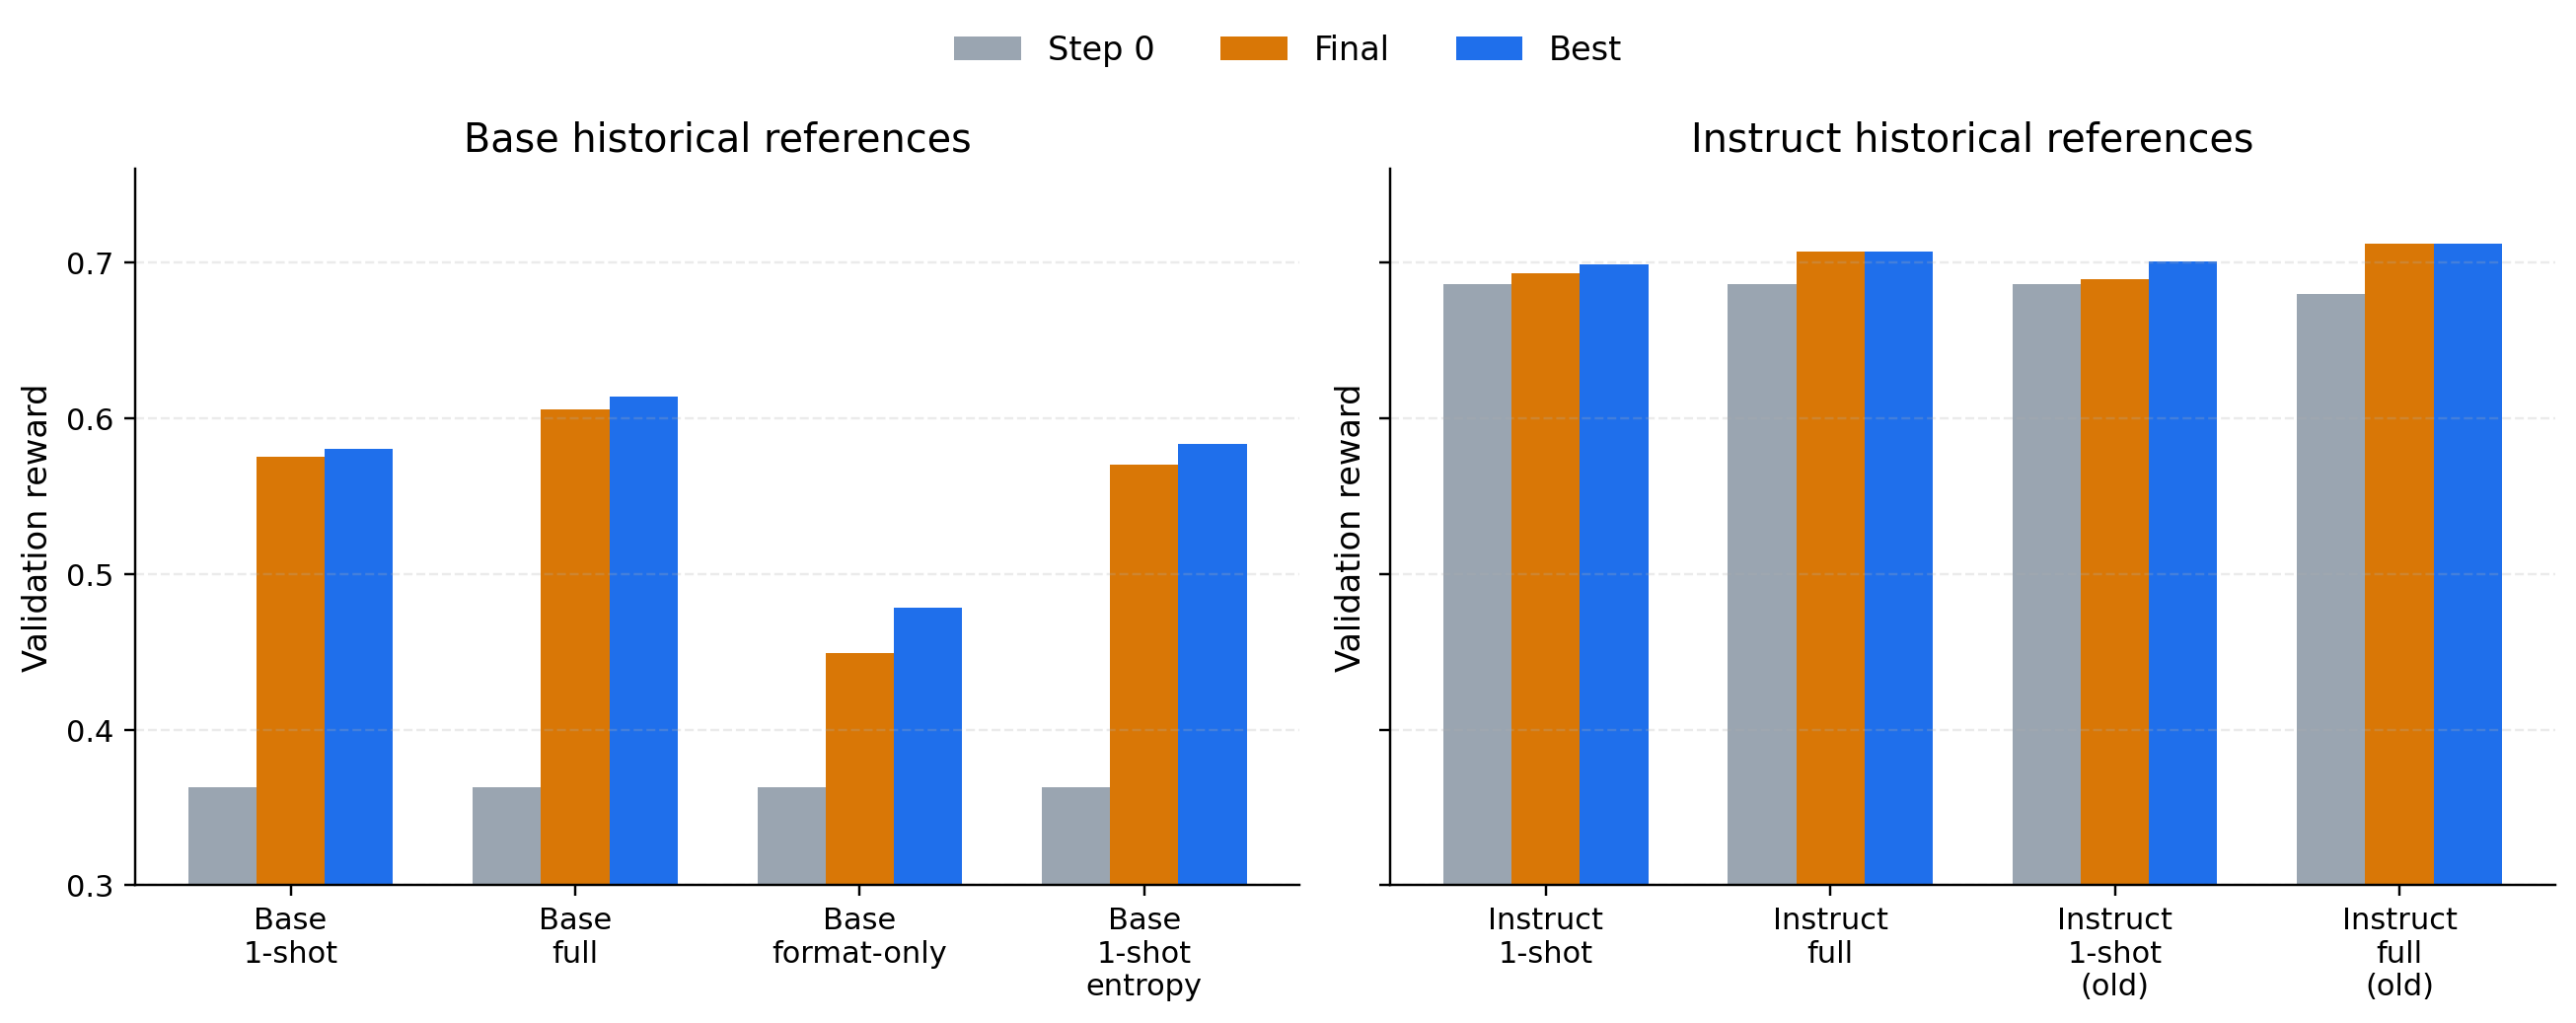
\includegraphics[width=\textwidth]{legacy-reference-panel.png}
    \caption{更早阶段历史参考实验的 step0、final 与 best 对比。该图表明，无论在 Base 还是 Instruct 家族中，\texttt{full} 训练通常都优于 \texttt{1-shot}；同时，Base 家族中的格式约束主导参考明显弱于常规奖励路径。}
    \label{fig:legacy-reference-main}
\end{figure}

图~\ref{fig:legacy-reference-main} 因而承担了正文里的一个特殊角色：它不是正式主结论的来源，而是对主结论进行“外部一致性”补强。对一篇正式 paper 而言，这类材料的价值在于，它可以避免正文叙事完全建立在单一最终矩阵之上，使“Base 更敏感于训练范式和奖励结构、Instruct 整体收益更温和”这一判断具有更宽的经验基础。

\section{主结果：1-shot GRPO 是否有效}

\subsection{总体趋势：Base 收益显著，Instruct 收益有限}

从表~\ref{tab:main-results} 可以直接看到两个强信号。第一，Base 模型在多个完整实验中都表现出接近 0.20 的绝对分数提升，这说明 1-shot GRPO 在弱先验数学模型上确实能够产生稳定而显著的收益。第二，Instruct 模型的改进明显更小，其结果更像在高性能附近做微调，而不是发生结构性变化。这与我们在方法部分提出的先验差异假设高度一致。

\begin{figure}[H]
    \centering
    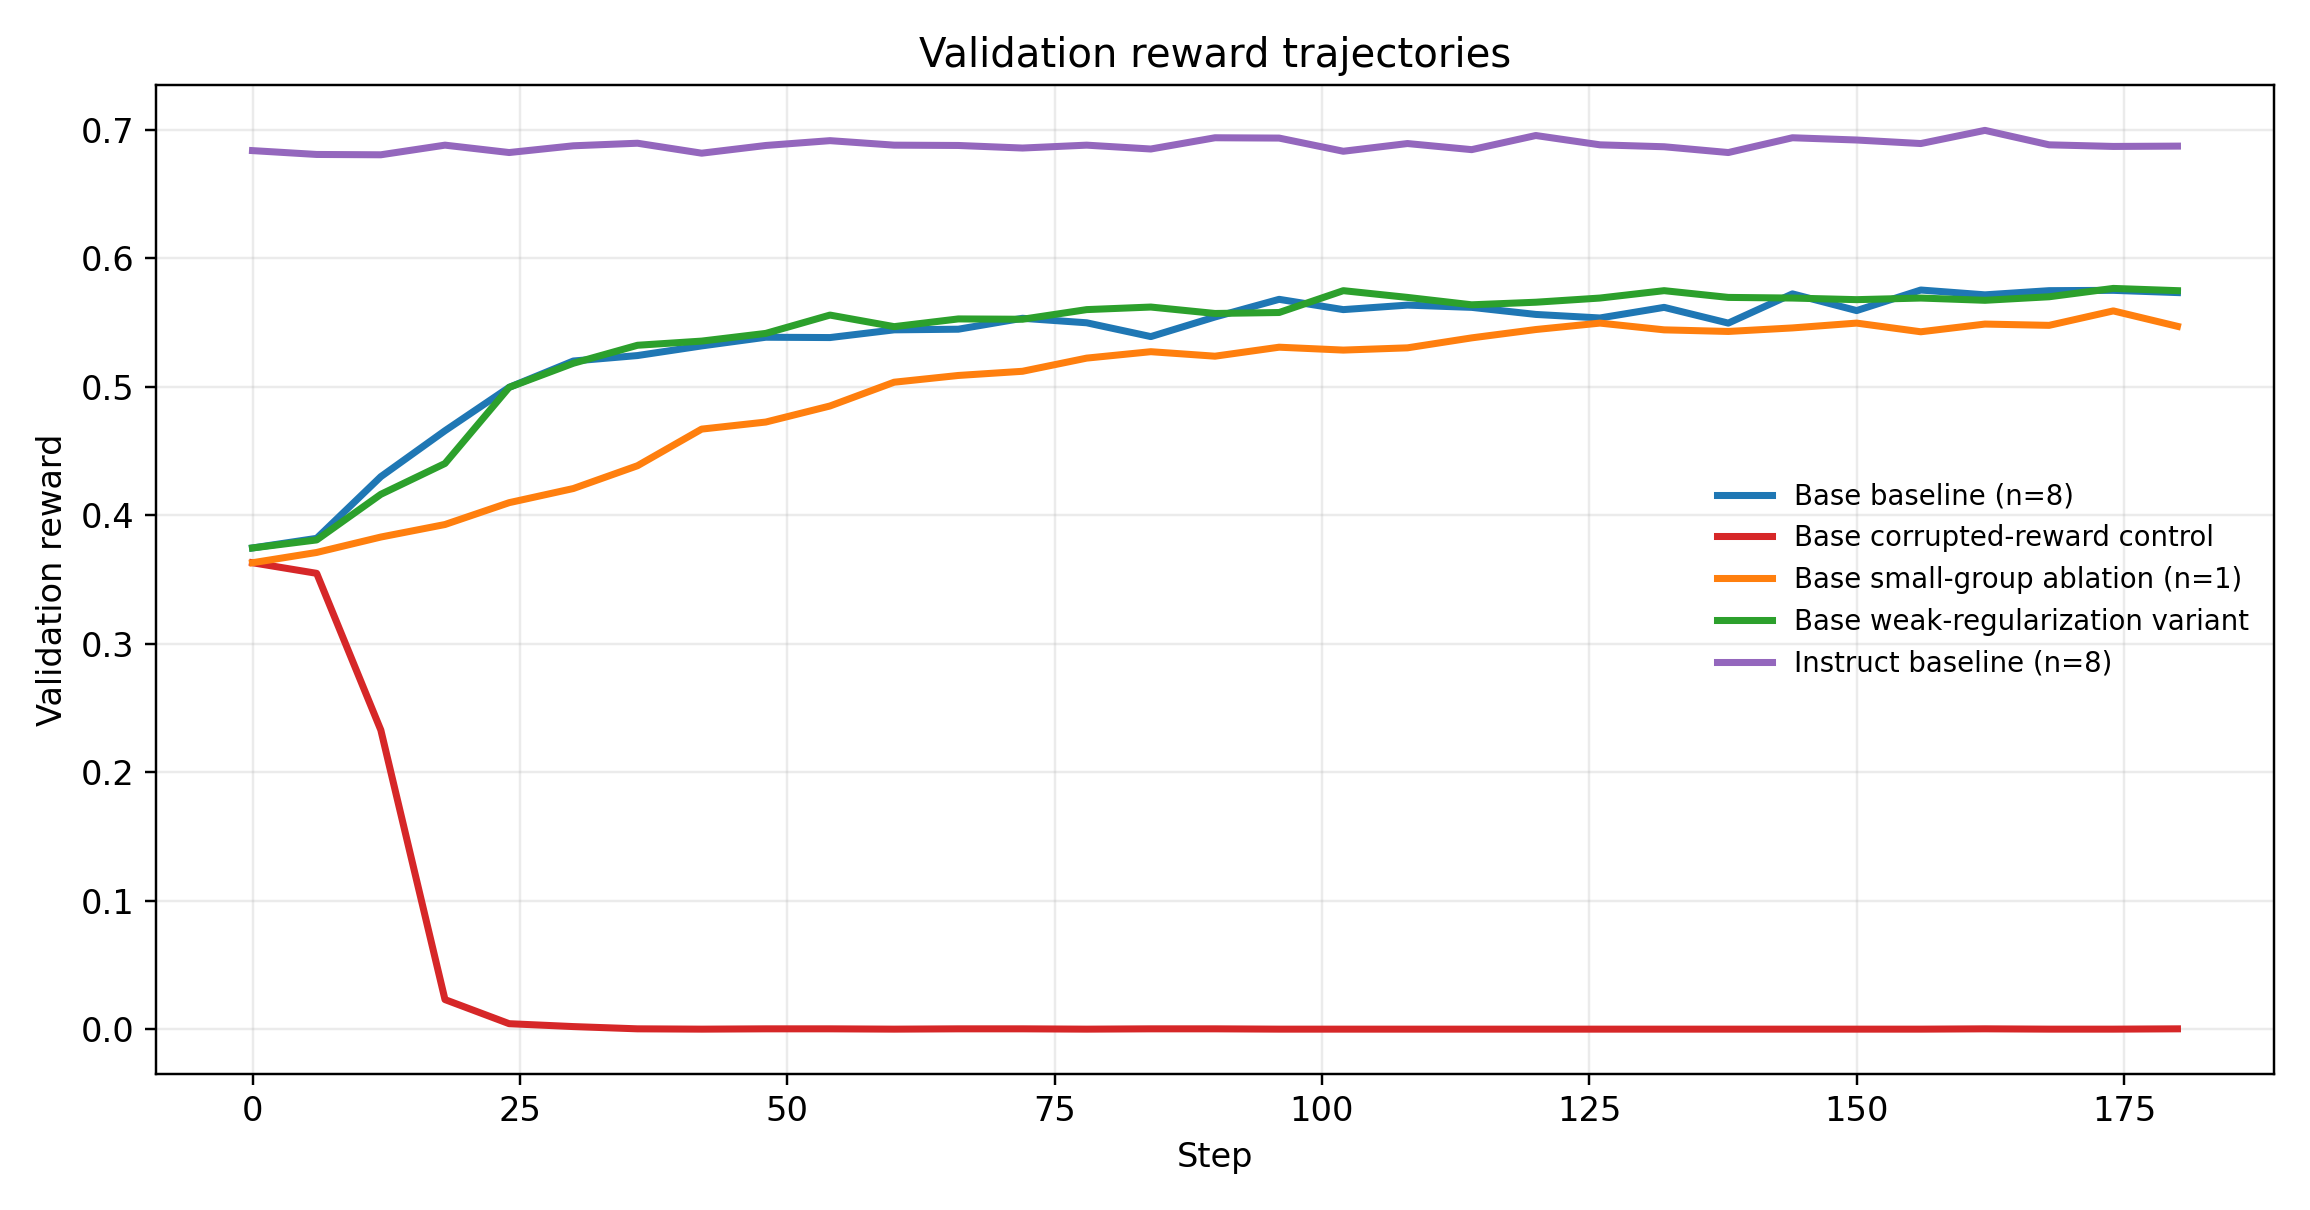
\includegraphics[width=\textwidth]{score-all-static.png}
    \caption{五个正式实验的 validation score 随训练 step 的变化。Base clean 实验整体抬升明显，而严格的破坏性奖励控制实验则快速坍缩。}
    \label{fig:all-score-curves}
\end{figure}

图~\ref{fig:all-score-curves} 强化了表格中的结论。Base 系列从较低起点快速爬升，并在中后期进入相对平稳的高位区间；Instruct 系列则从一开始就处于较高水平，后续训练带来的变化幅度明显更小。这意味着不能用同一个收益尺度评价两类模型。对于 Base 模型，训练是在帮助它摆脱“高熵、长拖尾、低置信”的初始状态；而对于 Instruct 模型，训练更像对已有好分布做细修整。

\subsection{Base 模型：收益大且具有一致性}

\texttt{Base baseline (n=8)} 从 0.3745 提升到 0.5733，说明标准设定下的 1-shot GRPO 已经足以把基础数学模型从“不够稳定可用”的状态拉升到更具实用性的区间。更值得注意的是，这一收益并不是孤例。\texttt{Base weak-regularization variant} 的 final score 为 0.5747，与标准基线非常接近；而新的严格控制实验 \texttt{Base corrupted-reward control} 却从 0.3630 快速坍缩到 0.00025。二者放在一起，恰好形成一组更有解释力的对照：当奖励结构与 clean baseline 保持同向时，Base 模型的收益具有较强可重复性；而当奖励信号被系统性破坏后，这种收益不会自然出现。

\begin{figure}[H]
    \centering
    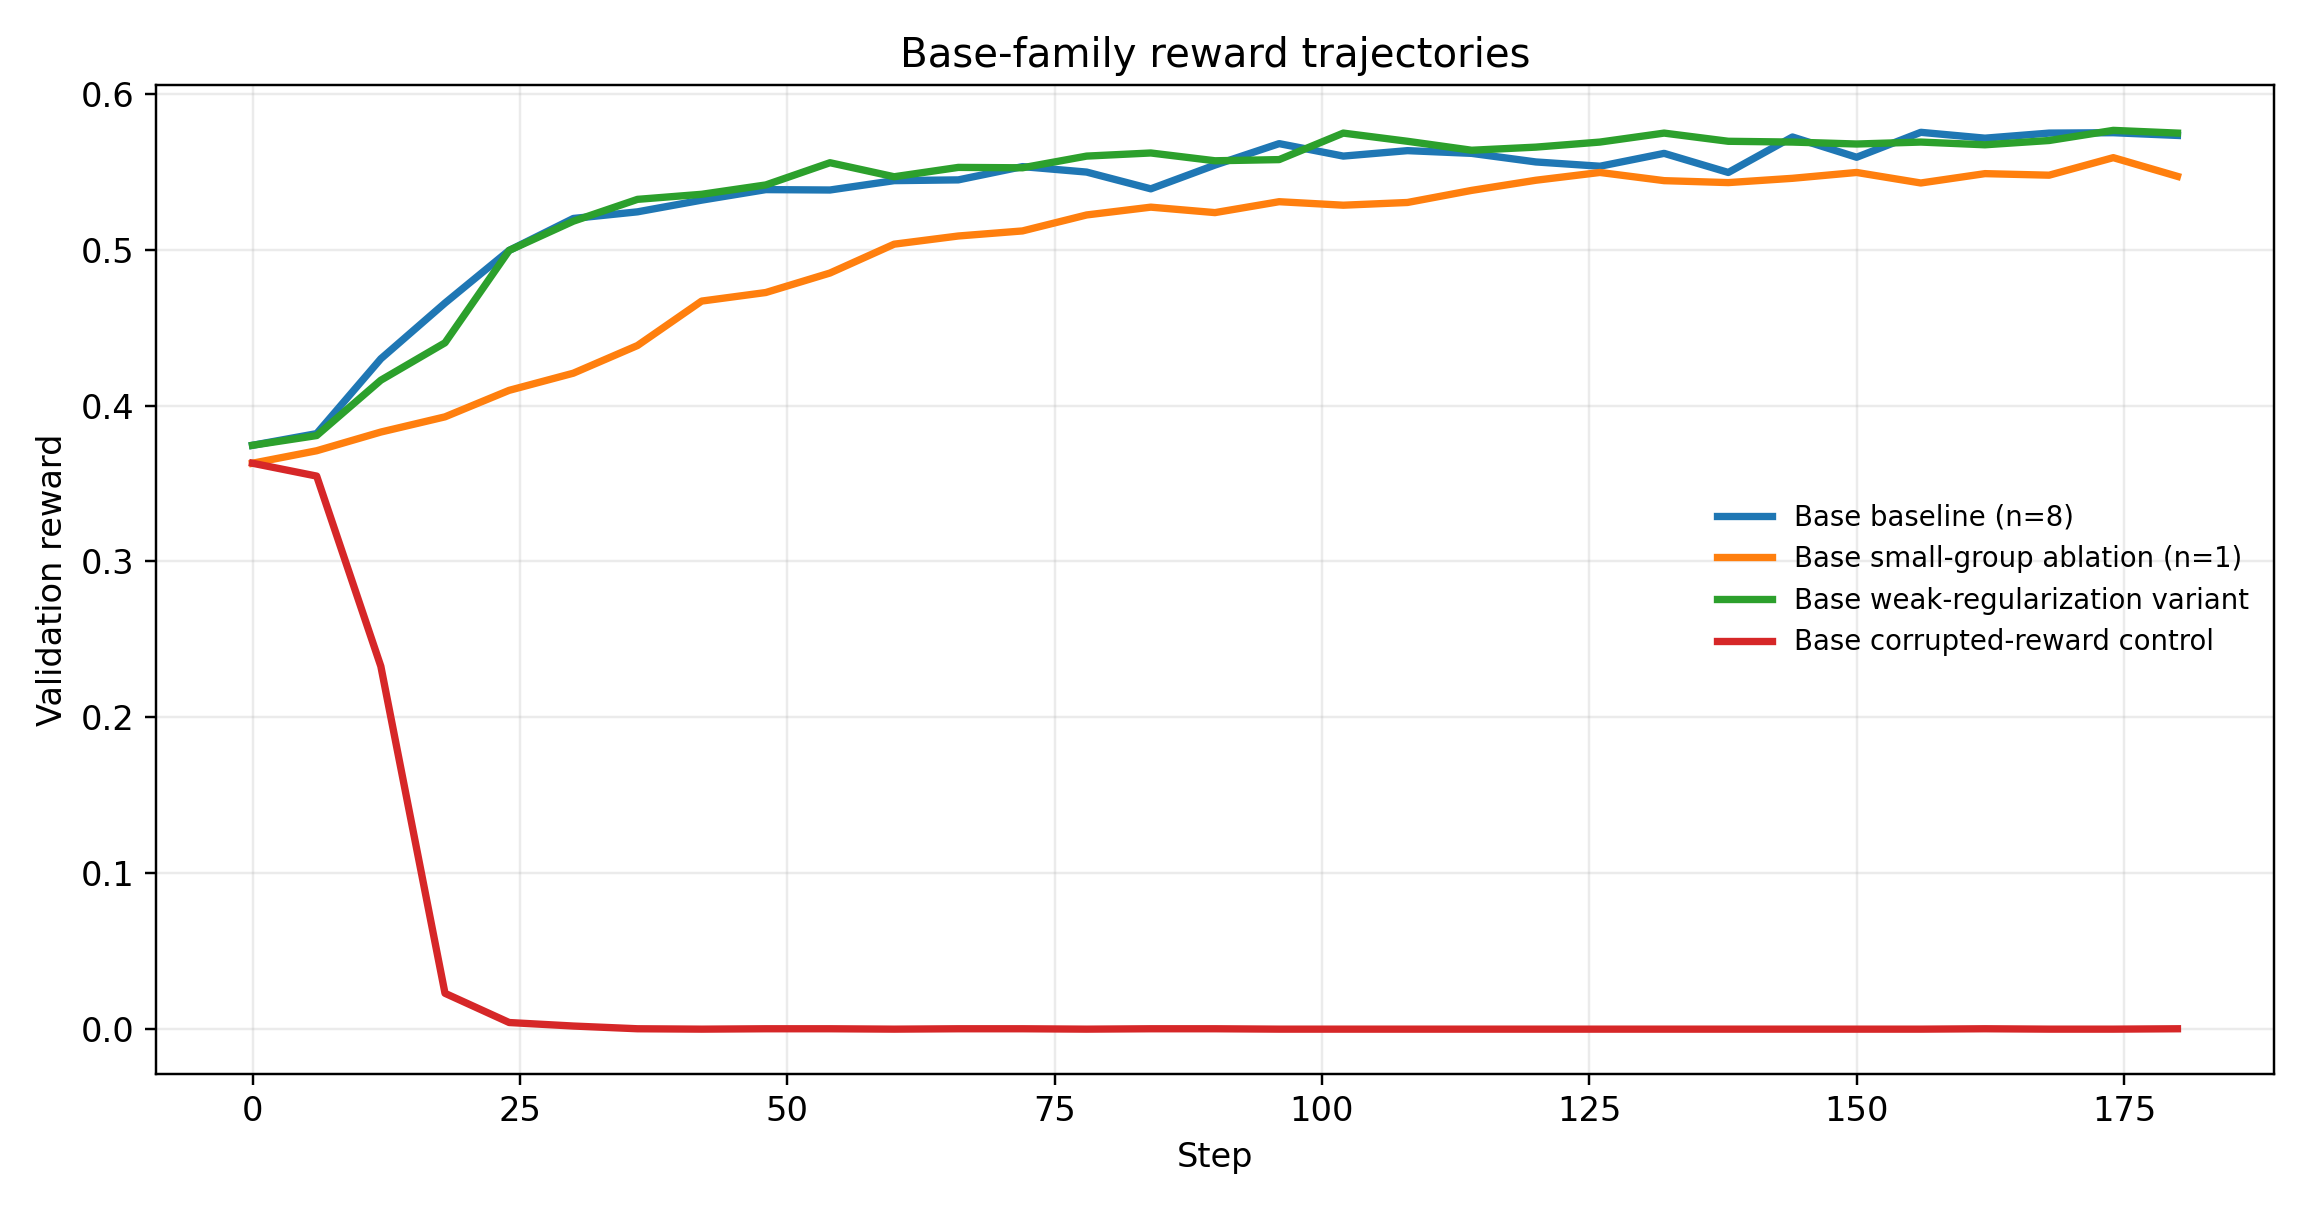
\includegraphics[width=\textwidth]{score-base-static.png}
    \caption{Base 家族四个正式实验的主分数变化。三个 clean 方向实验表现出前中期快速上升，而严格破坏性控制实验则快速失稳。}
    \label{fig:base-score-curves}
\end{figure}

\begin{figure}[H]
    \centering
    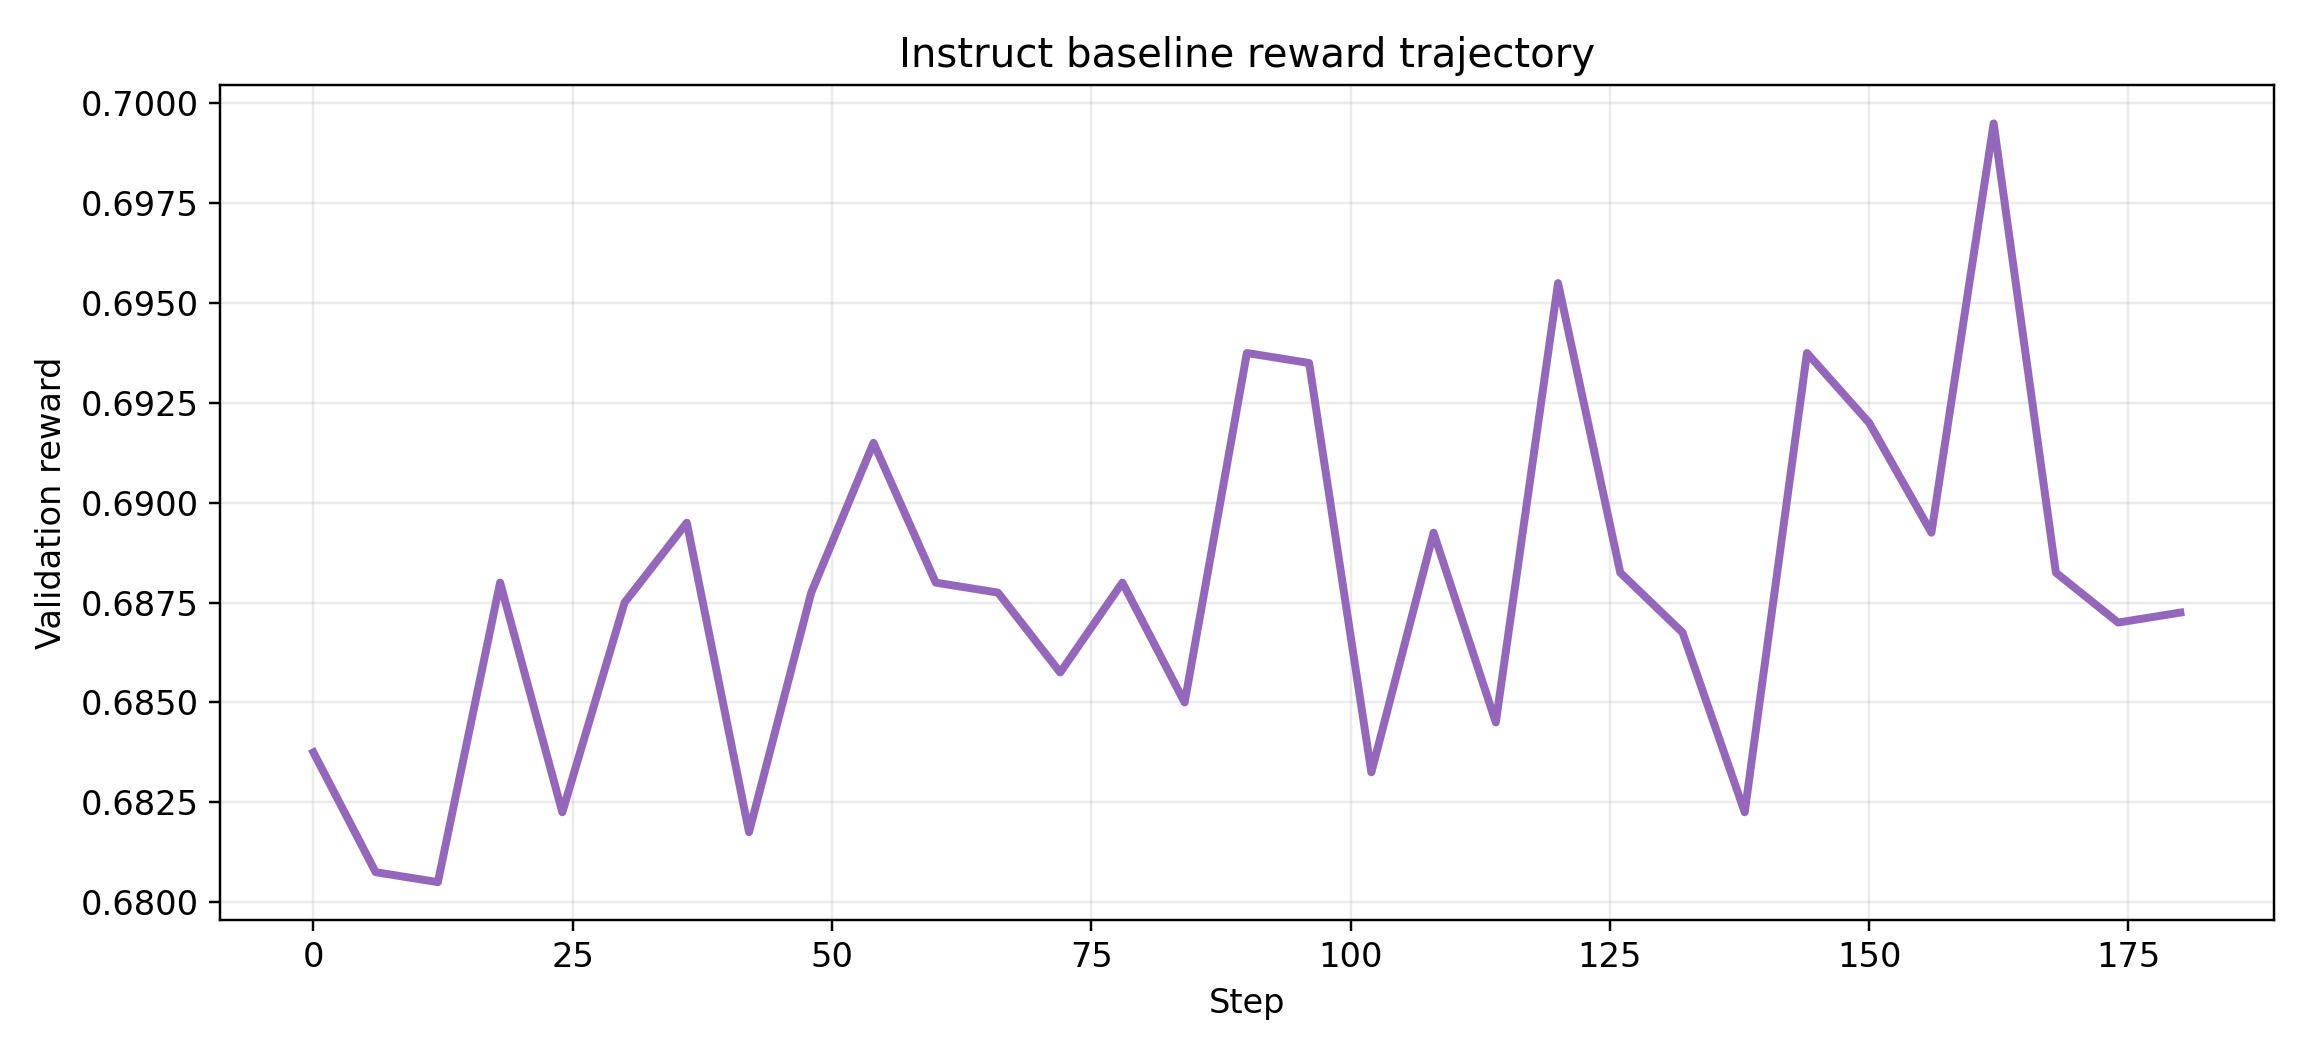
\includegraphics[width=\textwidth]{score-instruct-static.png}
    \caption{Instruct 家族基线实验的主分数变化。曲线整体维持在高位，训练主要表现为小幅波动与局部微调。}
    \label{fig:instruct-score-curves}
\end{figure}

图~\ref{fig:base-score-curves} 与图~\ref{fig:instruct-score-curves} 进一步说明，Base 家族的多个变体虽然有不同的后期波动，但都共享一种相似的学习形态：前中期快速上升，后期进入缓慢振荡；Instruct 家族则主要维持在高位窄幅波动。这提示在极低数据预算下，最佳 checkpoint 未必总是最终 checkpoint；在正式实验分析中区分二者是有意义的。

\subsection{Instruct 模型：高起点与小增益}

\texttt{Instruct baseline (n=8)} 在 \texttt{step 0} 就达到 0.6837，这一数值远高于 Base 模型的起点。训练后的 final score 为 0.6873，最佳 step 为 162，best score 为 0.6995。若只看数值，它仍然是一个有效实验，但其收益量级只有 0.0035，与 Base 模型约 0.20 的绝对提升完全不在同一量级。

因此，更准确的叙事不是“1-shot GRPO 对所有模型都同样有效”，而是“1-shot GRPO 的收益高度依赖于模型起点”。对于高先验 Instruct 模型，训练已经很难带来显著的结构性收益；对于先验较弱的 Base 模型，训练空间则大得多。

\subsection{最佳 step 与最终 step 不完全一致}

另一个不可忽略的观察是，多个实验的最佳分数并不出现在最终 \texttt{step 180}。例如，\texttt{Base baseline (n=8)} 的最好结果出现在 \texttt{step 156}，\texttt{Base weak-regularization variant} 出现在 \texttt{step 174}，\texttt{Instruct baseline (n=8)} 的最佳 step 则是 \texttt{162}。这一现象说明在当前训练预算下，模型的收益并不是单调累积的；相反，训练中后期可能进入高位波动区间。因此，在正式分析中区分“最终 checkpoint”和“最佳 checkpoint”是必要的。

\section{行为机制分析：训练究竟改了什么}

\subsection{Base 模型的收缩与稳定化}

如果只看 score，我们会知道 Base 模型变强了，但不知道它是如何变强的。行为指标给出了更直接的答案。表~\ref{tab:behavior-results} 显示，\texttt{Base baseline (n=8)} 在最终阶段的平均 response length 为 603.1，相比起点明显缩短；答案尾部置信度提升到 0.9331；低置信 token 比例降到 0.0325；token entropy 降到 0.1839；最终 EOS 概率上升到 0.9880。这组变化可以被概括为一句话：模型不再依赖冗长试探，而是开始更快地走向稳定闭合。

\begin{table}[H]
    \centering
    \caption{五个正式实验的最终行为指标汇总}
    \label{tab:behavior-results}
    \begin{tabular}{lcccccc}
        \toprule
        实验 & length & tail conf. & low-conf & entropy & EOS prob & top1 prob \\
        \midrule
        Base baseline (n=8) & 603.1 & 0.9331 & 0.0325 & 0.1839 & 0.9880 & 0.9354 \\
        Base small-group ablation (n=1) & 580.4 & 0.9003 & 0.0488 & 0.2811 & 0.9215 & 0.9227 \\
        Base weak-regularization variant & 578.6 & 0.9437 & 0.0294 & 0.1563 & 0.9738 & 0.9437 \\
        Base corrupted-reward control & 1192.4 & 0.0001 & 1.0000 & 11.5466 & 0.0009 & 0.0021 \\
        Instruct baseline (n=8) & 470.3 & 0.9571 & 0.0187 & 0.1322 & 0.9926 & 0.9634 \\
        \bottomrule
    \end{tabular}
\end{table}

这类变化与“能力注入”并不完全一致，却与“快速校准”高度吻合。若模型是在短期内真正学会新的数学知识，我们未必会同时看到长度缩短、结束概率上升和熵下降；但如果模型只是学会更稳定地组织原有解题习惯，那么这些指标恰好会一起变化。换句话说，训练收益更像是对分布进行重新整形，而不是为模型引入新的知识模块。

\begin{figure}[H]
    \centering
    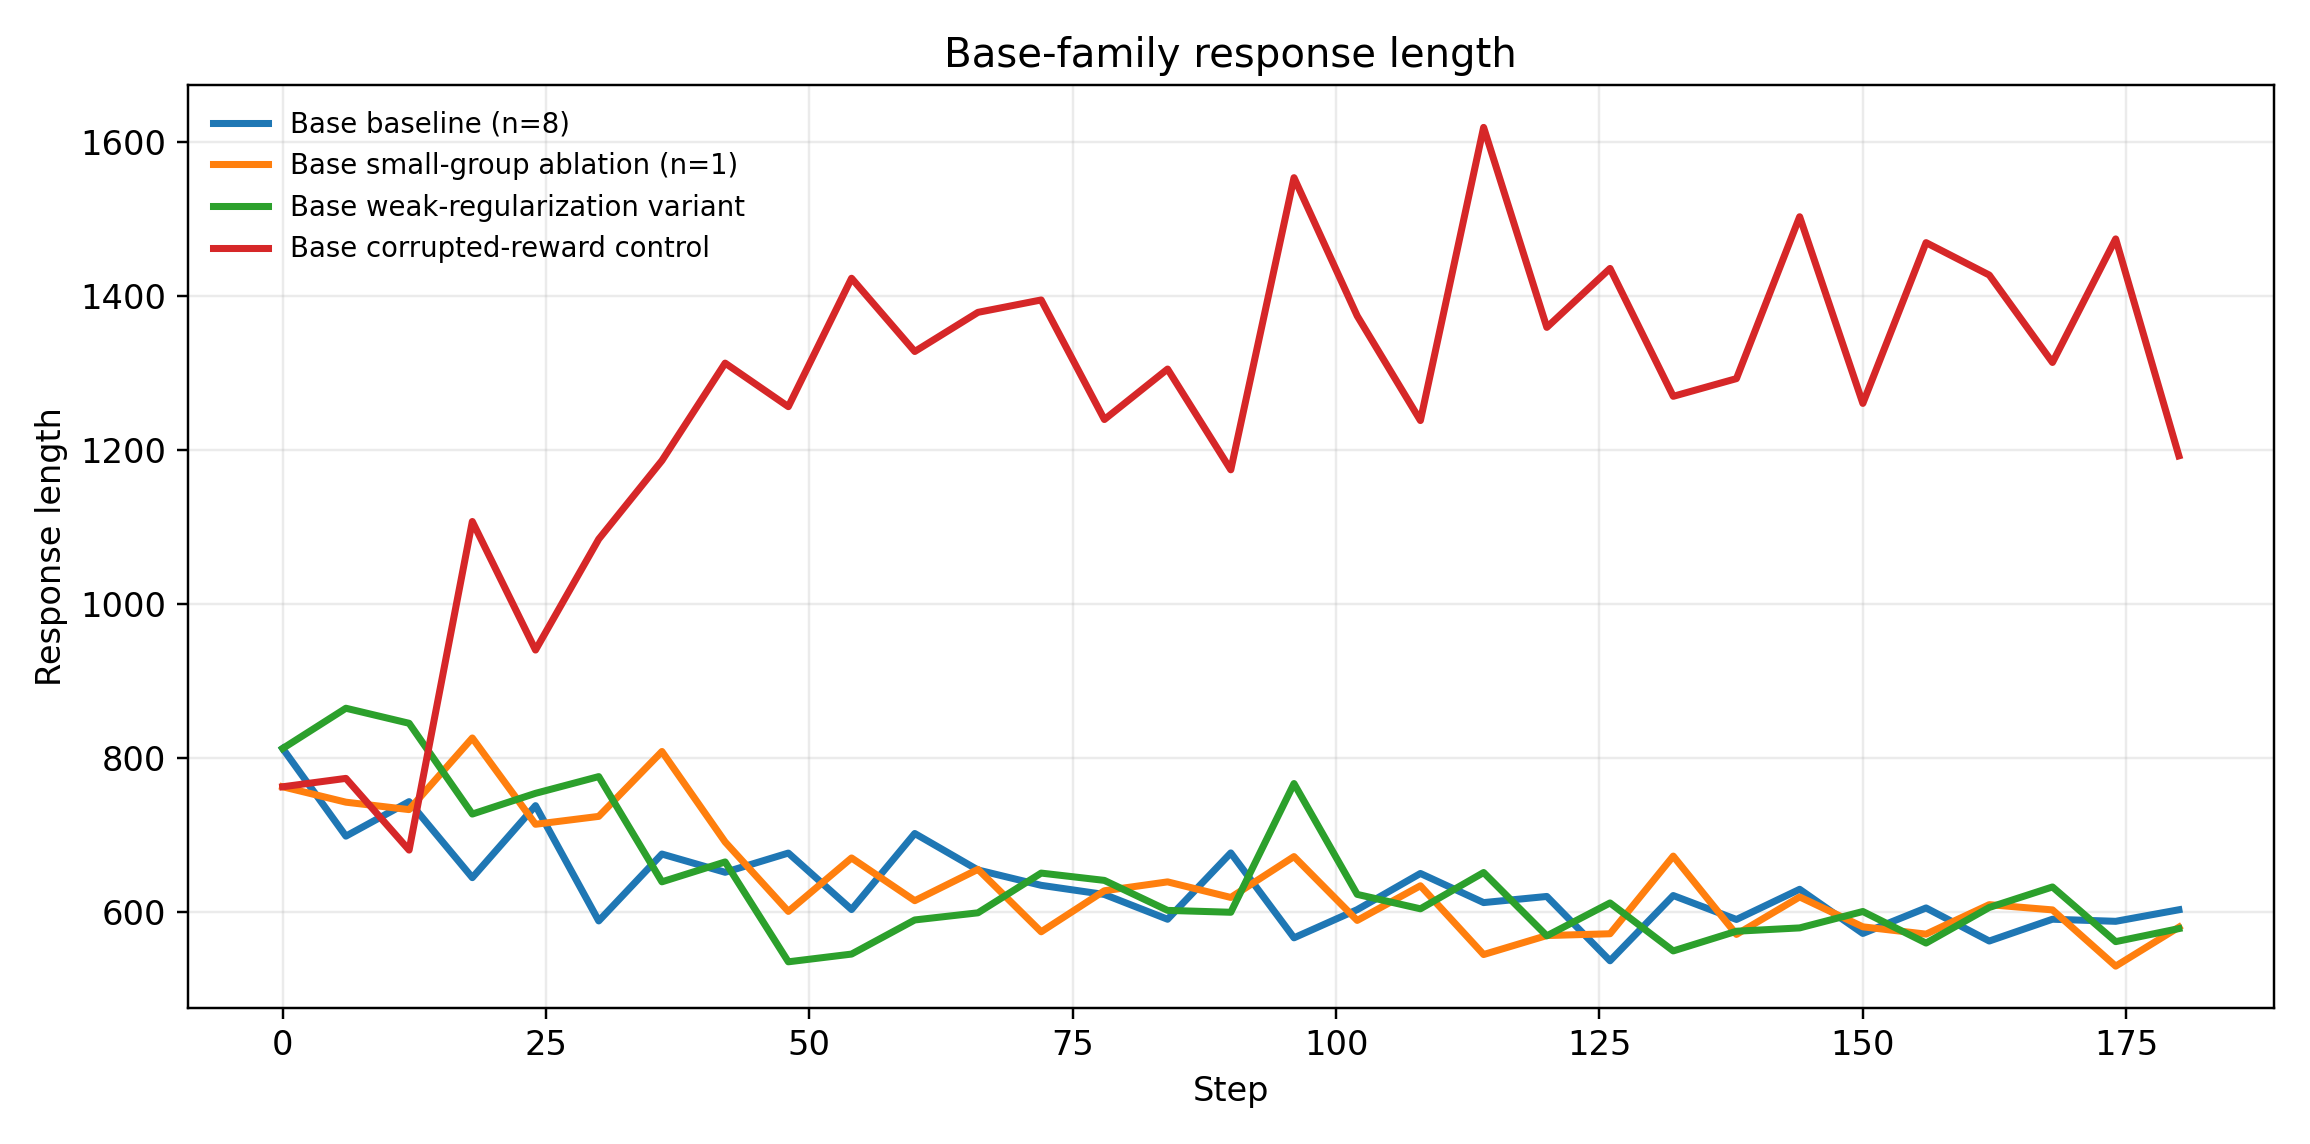
\includegraphics[width=\textwidth]{base-length-static.png}
    \caption{Base 家族四个正式实验的验证响应长度变化。clean 方向实验整体变短，而破坏性奖励控制实验则显著变长。}
    \label{fig:base-length-curves}
\end{figure}

\begin{figure}[H]
    \centering
    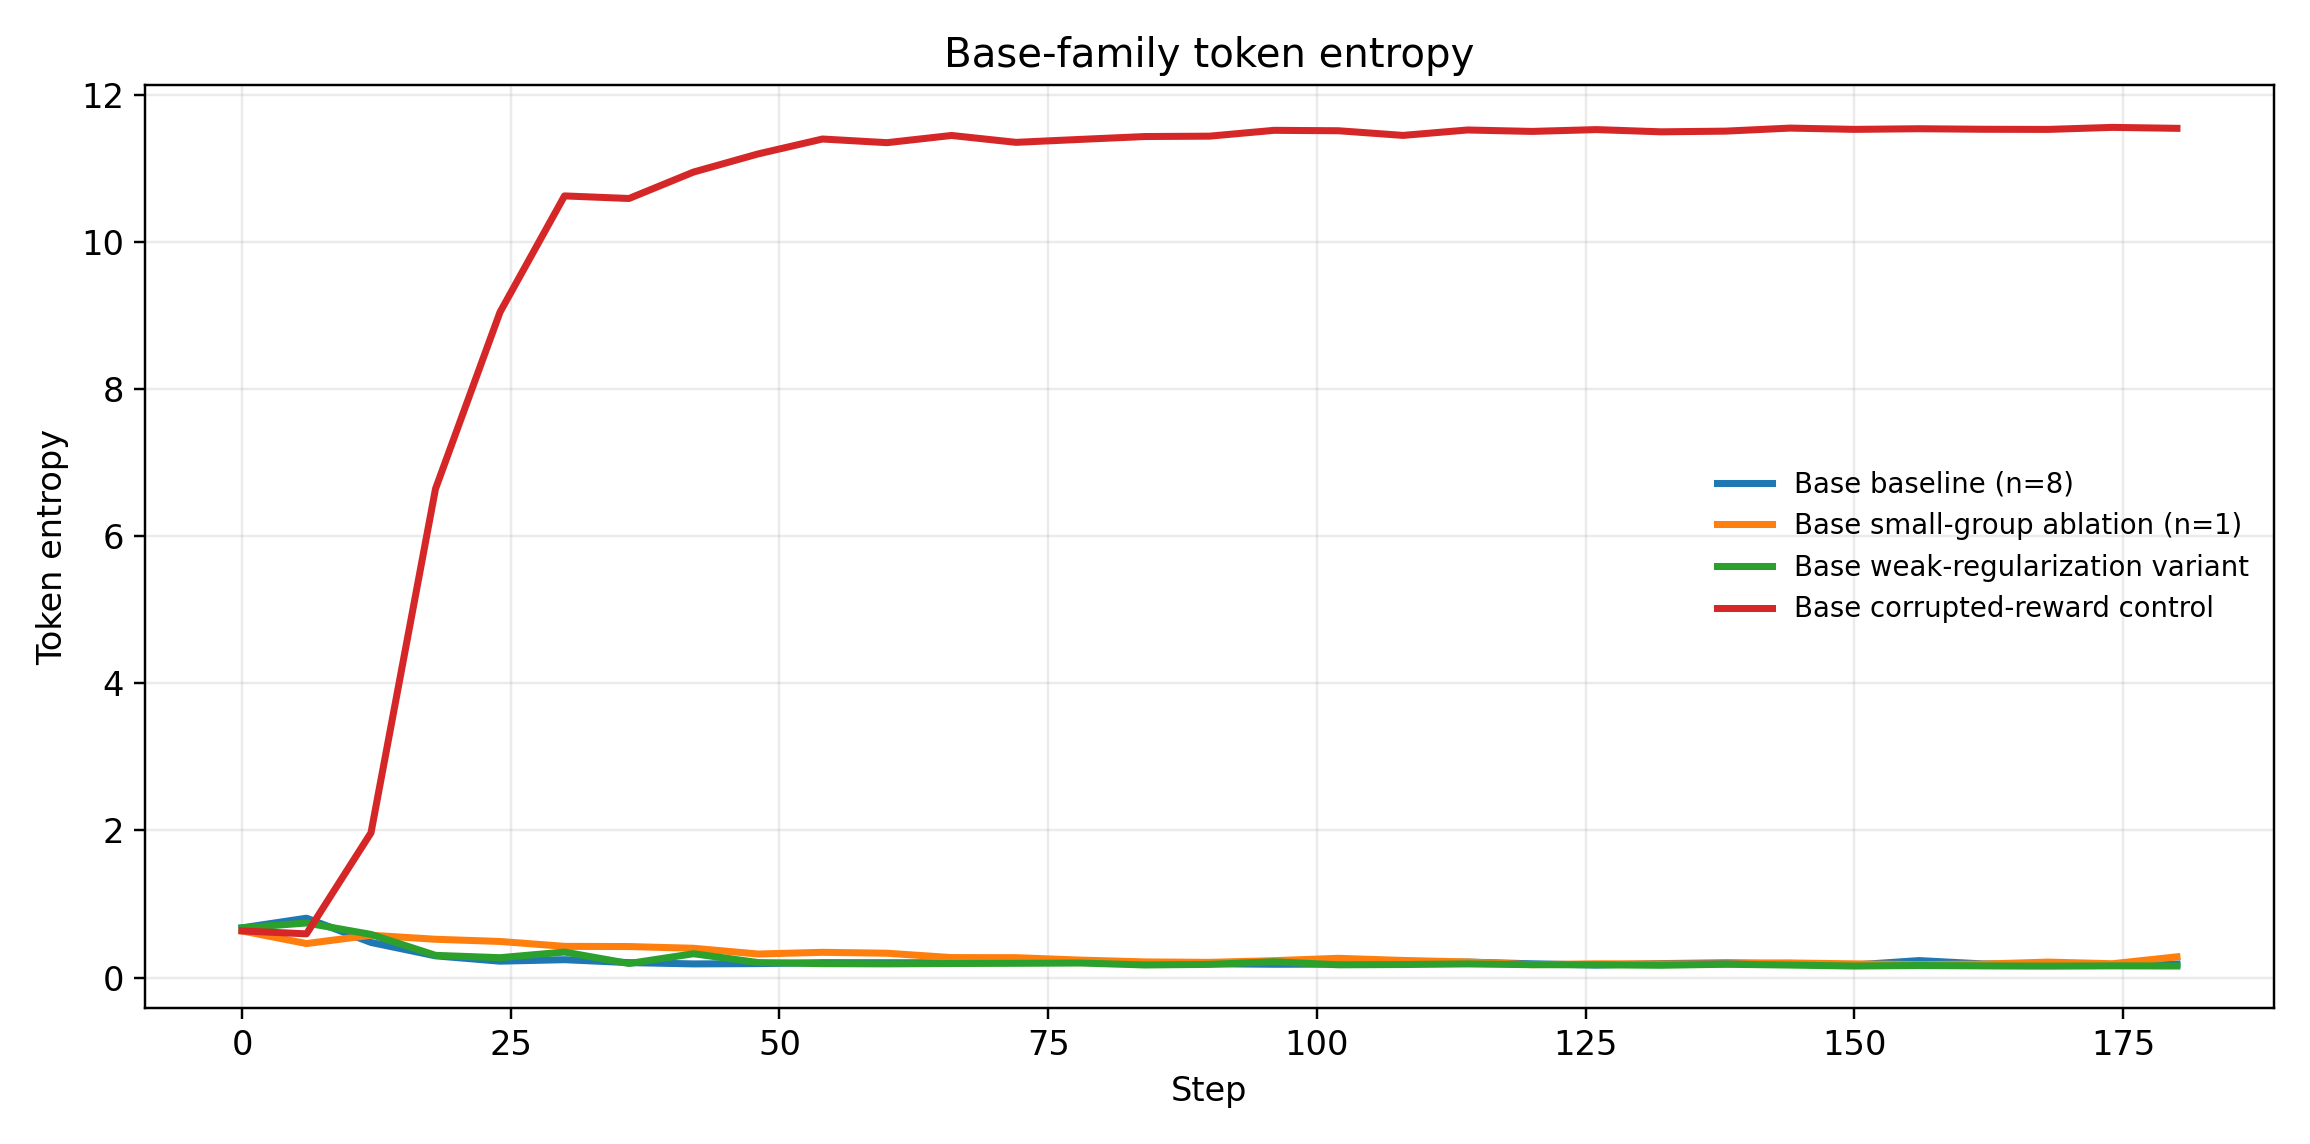
\includegraphics[width=\textwidth]{base-entropy-static.png}
    \caption{Base 家族四个正式实验的验证 token entropy 变化。clean 方向实验明显收缩，而破坏性控制实验出现熵爆炸。}
    \label{fig:base-entropy-curves}
\end{figure}

\begin{figure}[H]
    \centering
    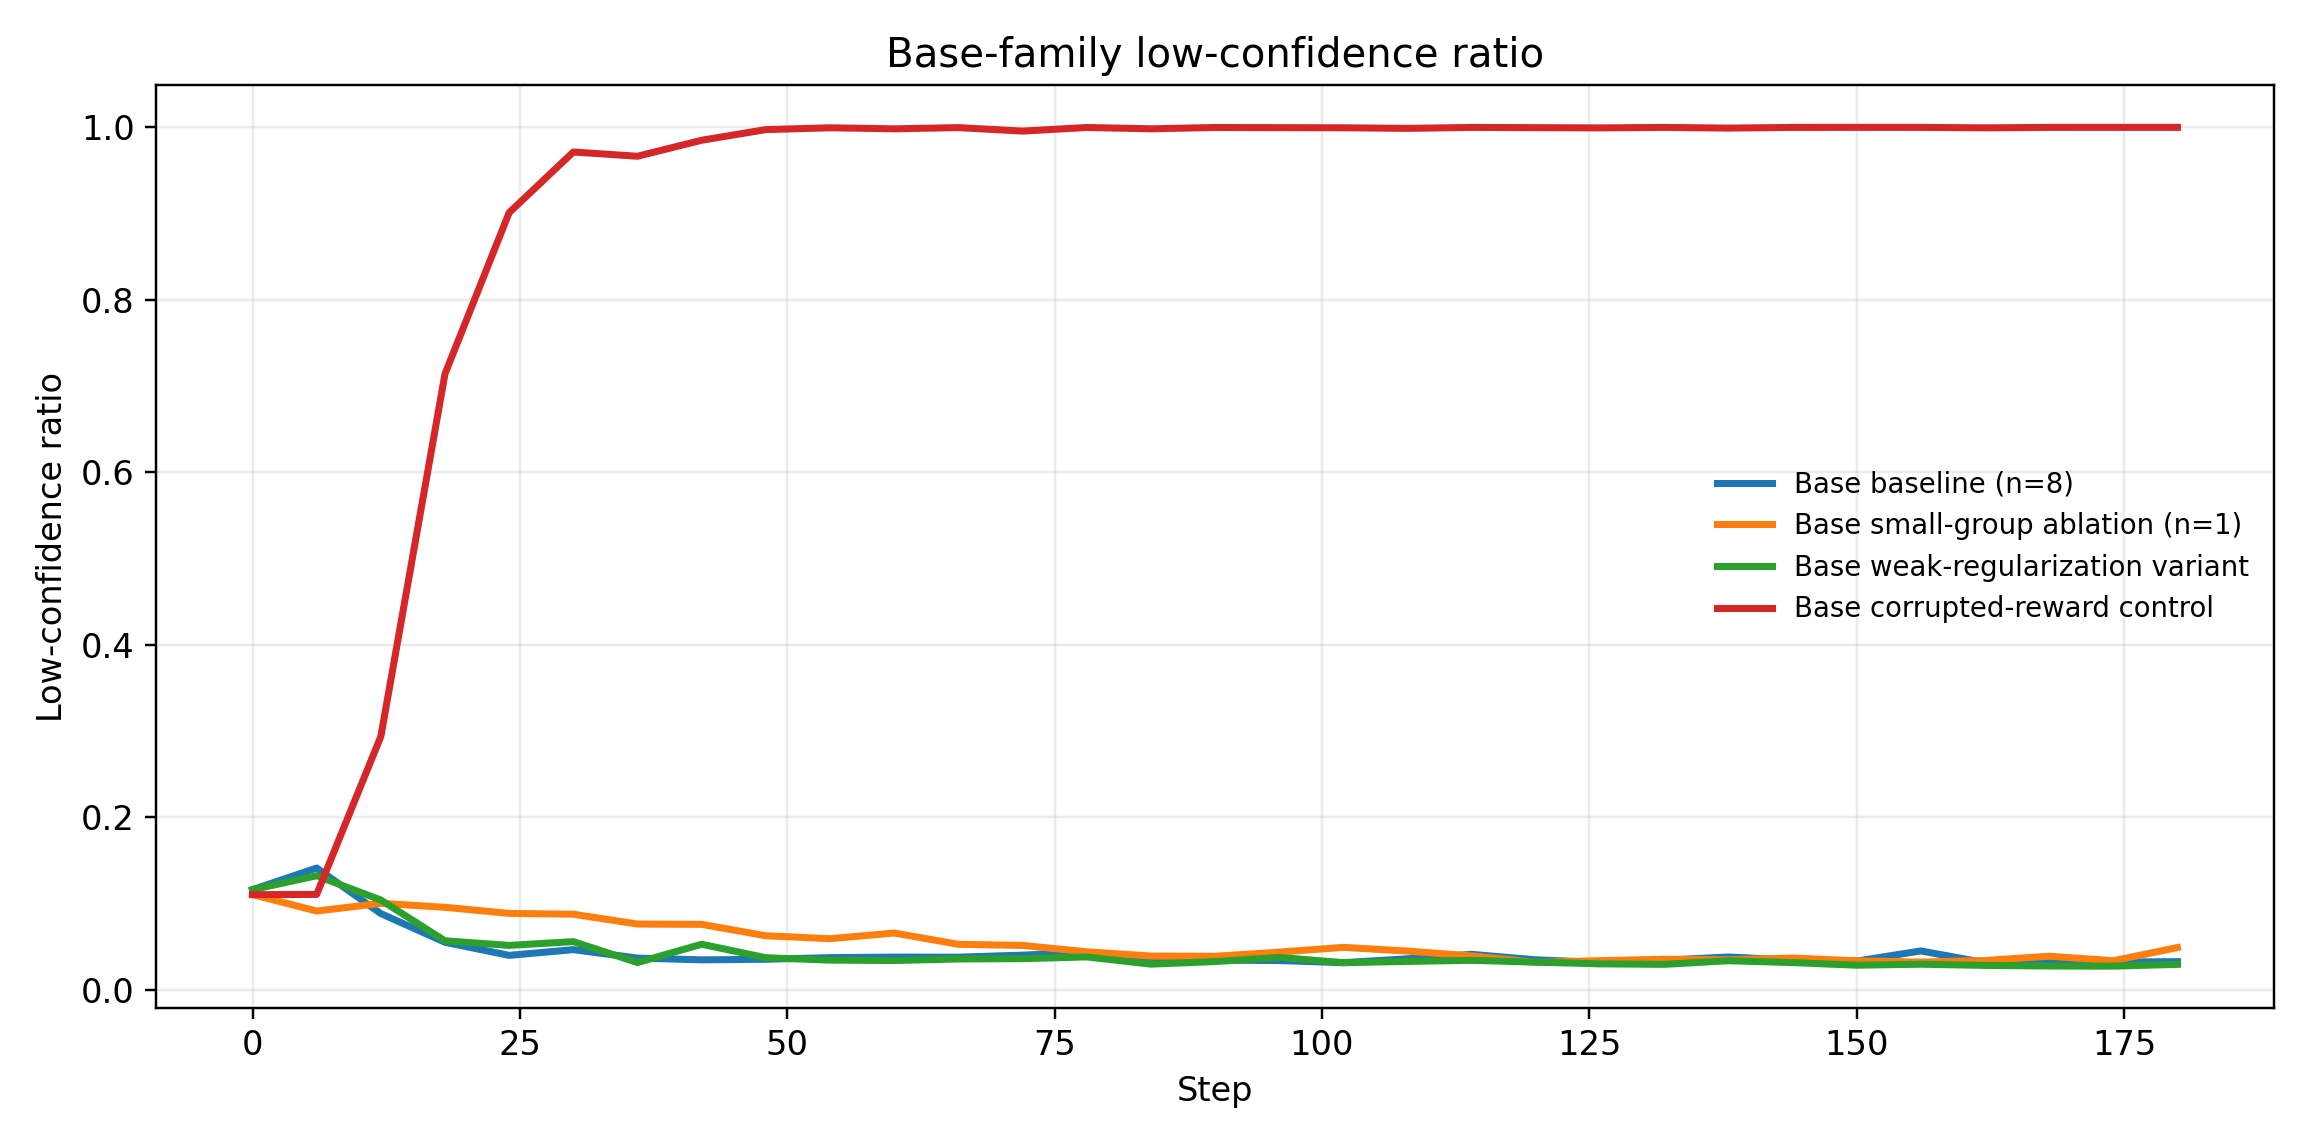
\includegraphics[width=\textwidth]{base-lowconf-static.png}
    \caption{Base 家族四个正式实验的低置信 token 比例变化。clean 方向实验持续下降，而破坏性控制实验迅速升至饱和。}
    \label{fig:base-lowconf-curves}
\end{figure}

\begin{figure}[H]
    \centering
    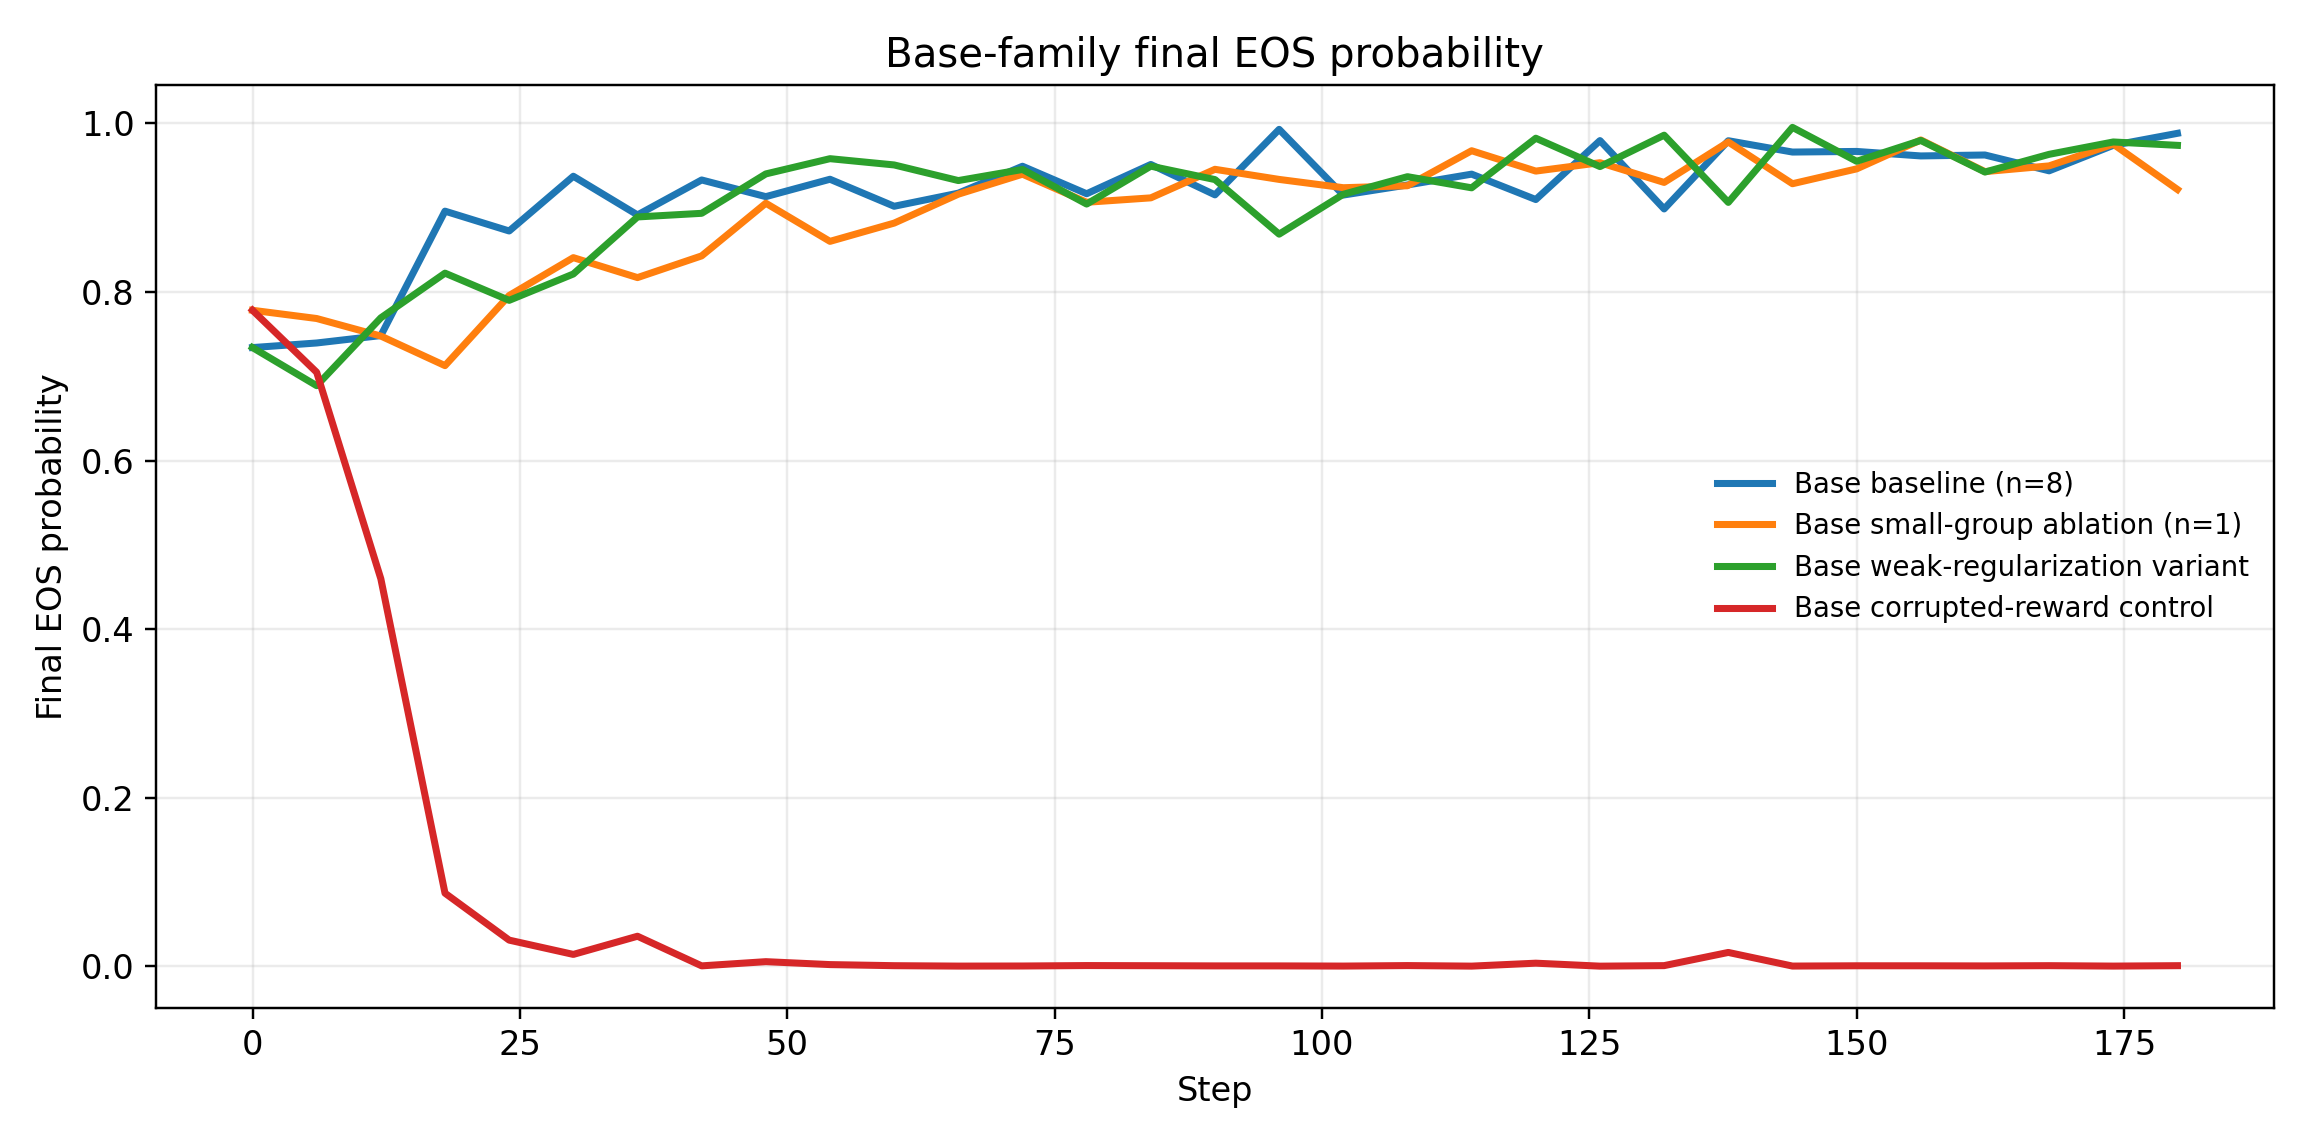
\includegraphics[width=\textwidth]{base-eos-static.png}
    \caption{Base 家族四个正式实验的最终 EOS 概率变化。clean 方向实验训练后更倾向于在合适位置结束，而破坏性控制实验则失去稳定闭合能力。}
    \label{fig:base-eos-curves}
\end{figure}

\begin{figure}[H]
    \centering
    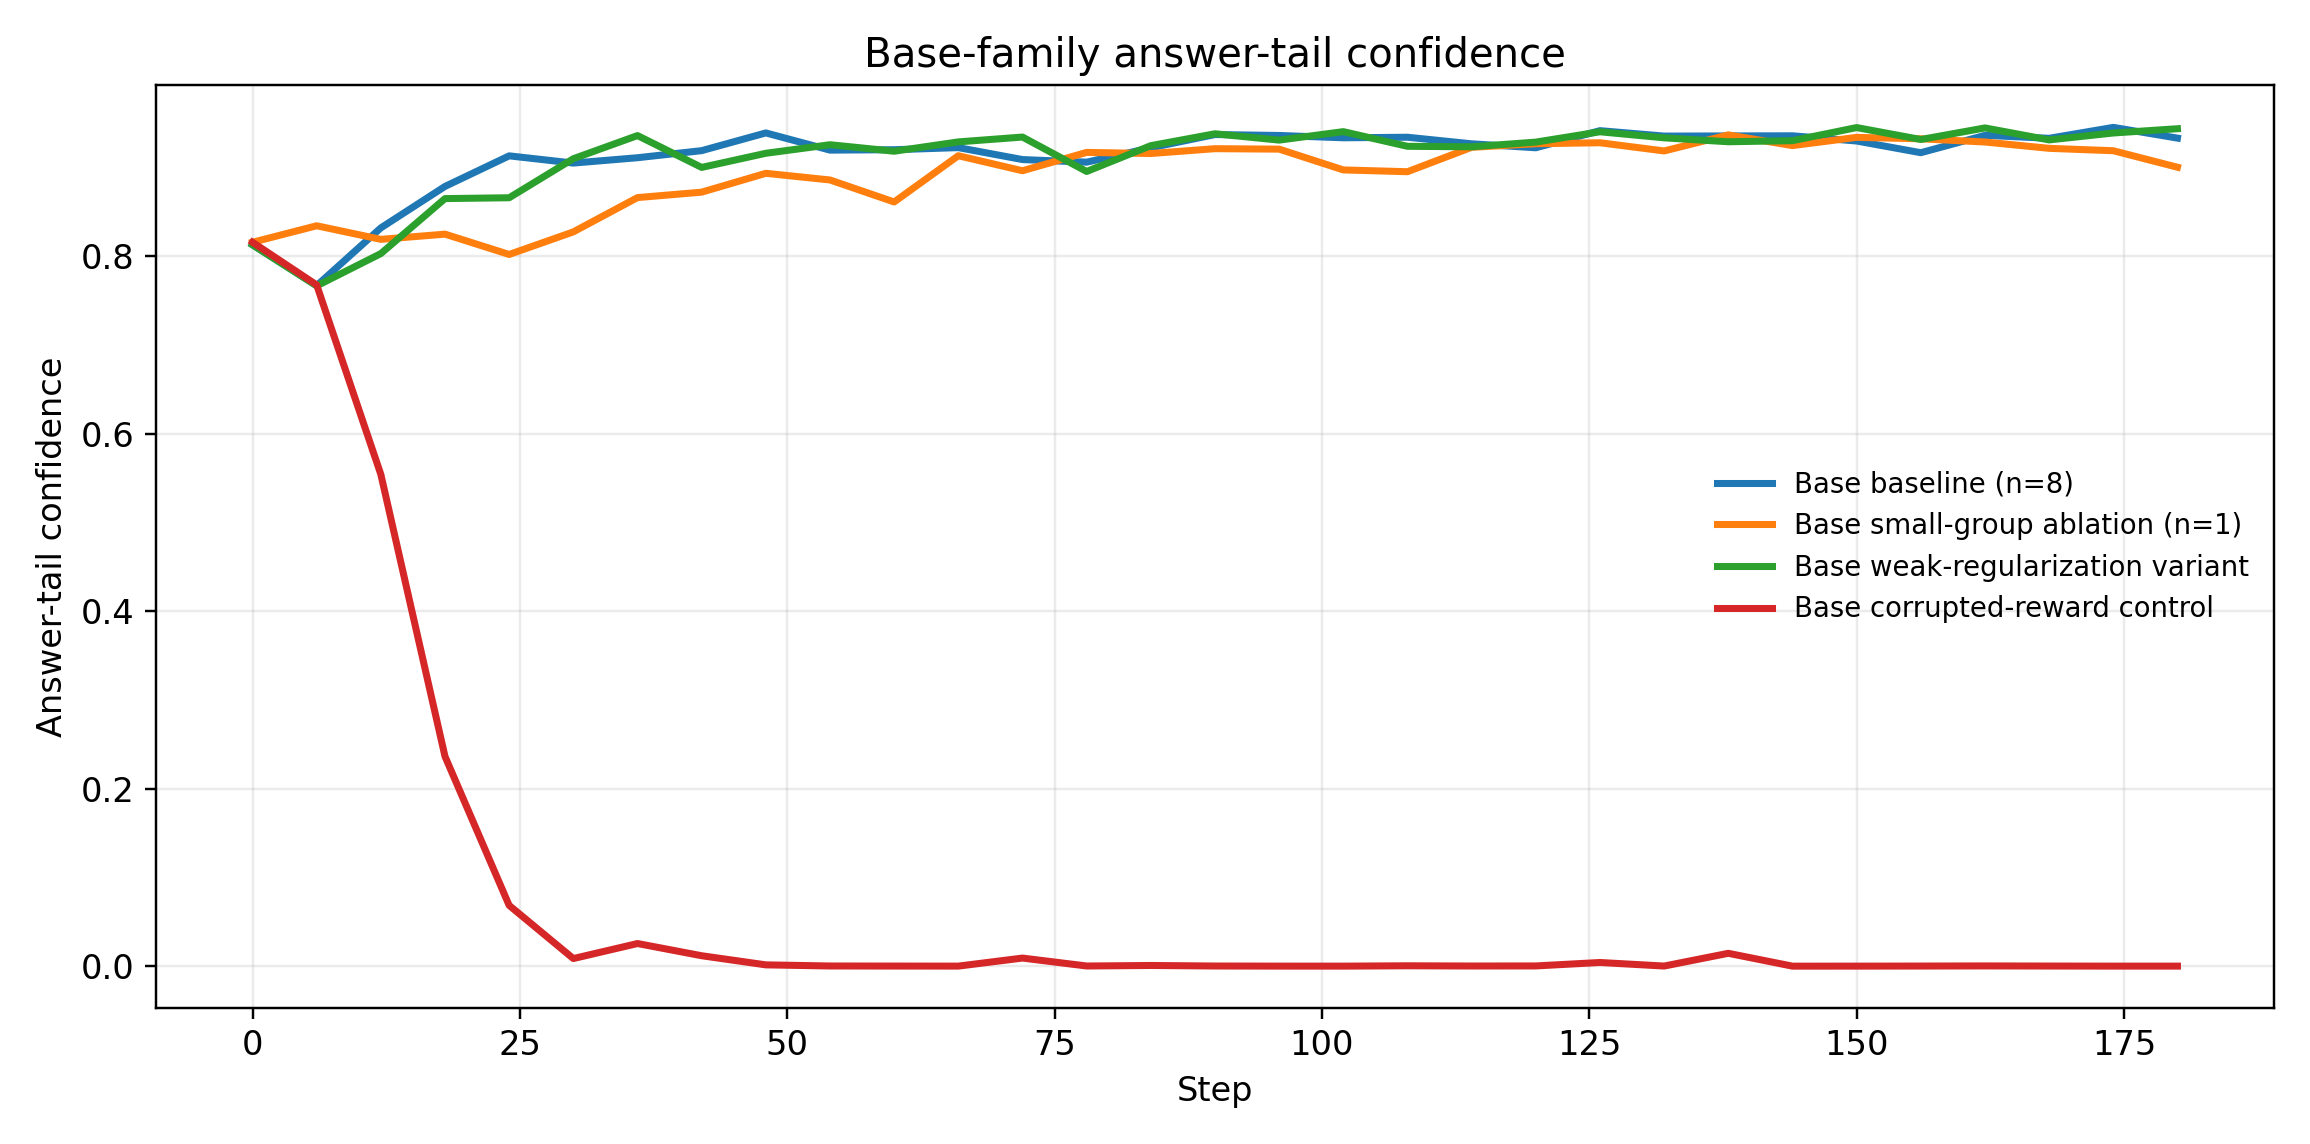
\includegraphics[width=\textwidth]{base-tailconf-static.png}
    \caption{Base 家族四个正式实验的答案尾部置信度变化。clean 方向实验在答案闭合附近置信度整体提高，而破坏性控制实验接近完全崩解。}
    \label{fig:base-tailconf-curves}
\end{figure}

\begin{figure}[H]
    \centering
    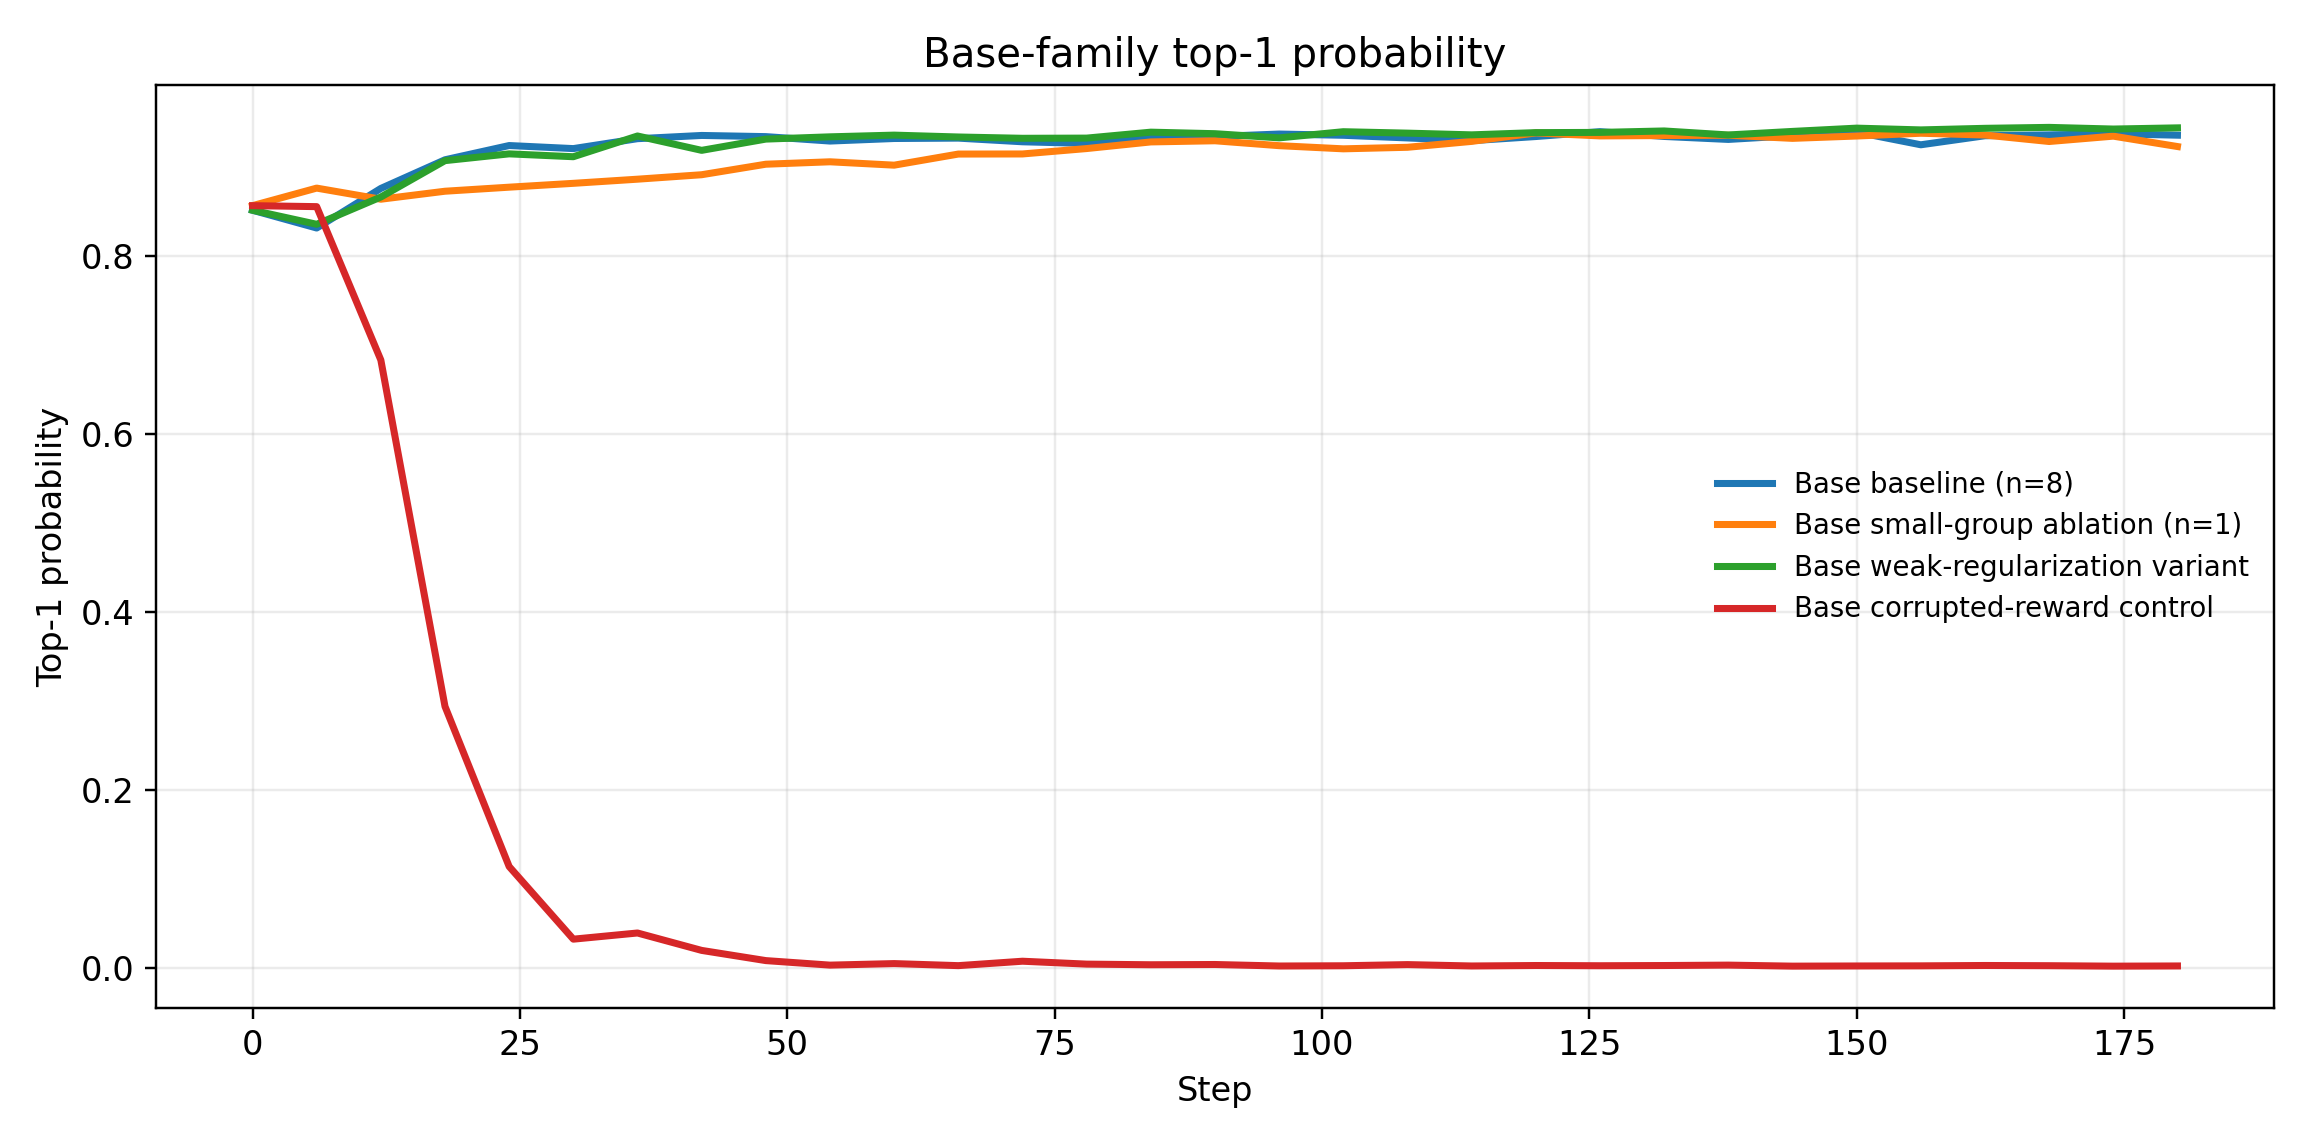
\includegraphics[width=\textwidth]{base-top1-static.png}
    \caption{Base 家族四个正式实验的平均 top-1 token 概率变化。clean 方向实验后期分布更加集中，而破坏性控制实验则迅速变得近乎均匀。}
    \label{fig:base-top1-curves}
\end{figure}

图~\ref{fig:base-length-curves} 到图~\ref{fig:base-top1-curves} 让这种行为变化变得更加直观。尤其值得关注的是 response length、tail confidence、top-1 probability 与 EOS probability 的联动：随着训练进行，Base 家族普遍变得更短，也更愿意在合适位置结束；与此同时，token entropy 与低置信 token 比例同步下降，而答案尾部置信度与平均 top-1 概率同步上升。这意味着模型不是靠“多说一点”提升分数，而是靠“更稳更准地结束”提升分数。对数学题这种最终答案明确、拖尾反而容易引入错误的任务而言，这一点尤其关键。

\subsection{动态统计进一步强化了上述判断}

训练与验证阶段的动态统计把前面的静态结果推进到了过程层面。与只看最终 checkpoint 不同，这些统计同时记录了训练期的 \texttt{actor/entropy} 和验证期的聚合 token 指标，因此能更直接地区分“真正变得更稳定的策略”和“仅在终点分数上略占优势的策略”。表~\ref{tab:dynamic-summary} 汇总了五个正式实验从起点到终点的核心变化。

\begin{table}[H]
    \centering
    \caption{训练与验证动态统计摘要（起点$\rightarrow$终点）}
    \label{tab:dynamic-summary}
    \begin{threeparttable}
    \small
    \begin{tabularx}{\textwidth}{>{\raggedright\arraybackslash}Xccccc}
        \toprule
        实验 & actor entropy & val token entropy & low-conf ratio & val length & top1 prob \\
        \midrule
        Base baseline (n=8) & 0.346$\rightarrow$0.116 & 0.660$\rightarrow$0.202 & 0.115$\rightarrow$0.037 & 812.5$\rightarrow$603.1 & 0.854$\rightarrow$0.932 \\
        Base small-group ablation (n=1) & 0.641$\rightarrow$0.085 & 0.532$\rightarrow$0.317 & 0.095$\rightarrow$0.051 & 762.8$\rightarrow$580.4 & 0.873$\rightarrow$0.921 \\
        Base weak-regularization variant & 0.346$\rightarrow$0.091 & 0.660$\rightarrow$0.156 & 0.115$\rightarrow$0.030 & 812.5$\rightarrow$578.6 & 0.854$\rightarrow$0.944 \\
        Base corrupted-reward control & 0.376$\rightarrow$11.594 & 0.633$\rightarrow$11.547 & 0.110$\rightarrow$1.000 & 762.8$\rightarrow$1192.4 & 0.856$\rightarrow$0.002 \\
        Instruct baseline (n=8) & 0.118$\rightarrow$0.062 & 0.111$\rightarrow$0.156 & 0.017$\rightarrow$0.022 & 473.2$\rightarrow$470.3 & 0.964$\rightarrow$0.961 \\
        \bottomrule
    \end{tabularx}
    \begin{tablenotes}[flushleft]
        \footnotesize
        \item 注：起点取第一个有值的训练或验证 step，终点取最终验证 step。验证 token 指标来自聚合 token diagnostics，每个 step 分析 64 个样本；当前五个正式实验的覆盖率均约为 1.6\%。
    \end{tablenotes}
    \end{threeparttable}
\end{table}

\begin{figure}[H]
    \centering
    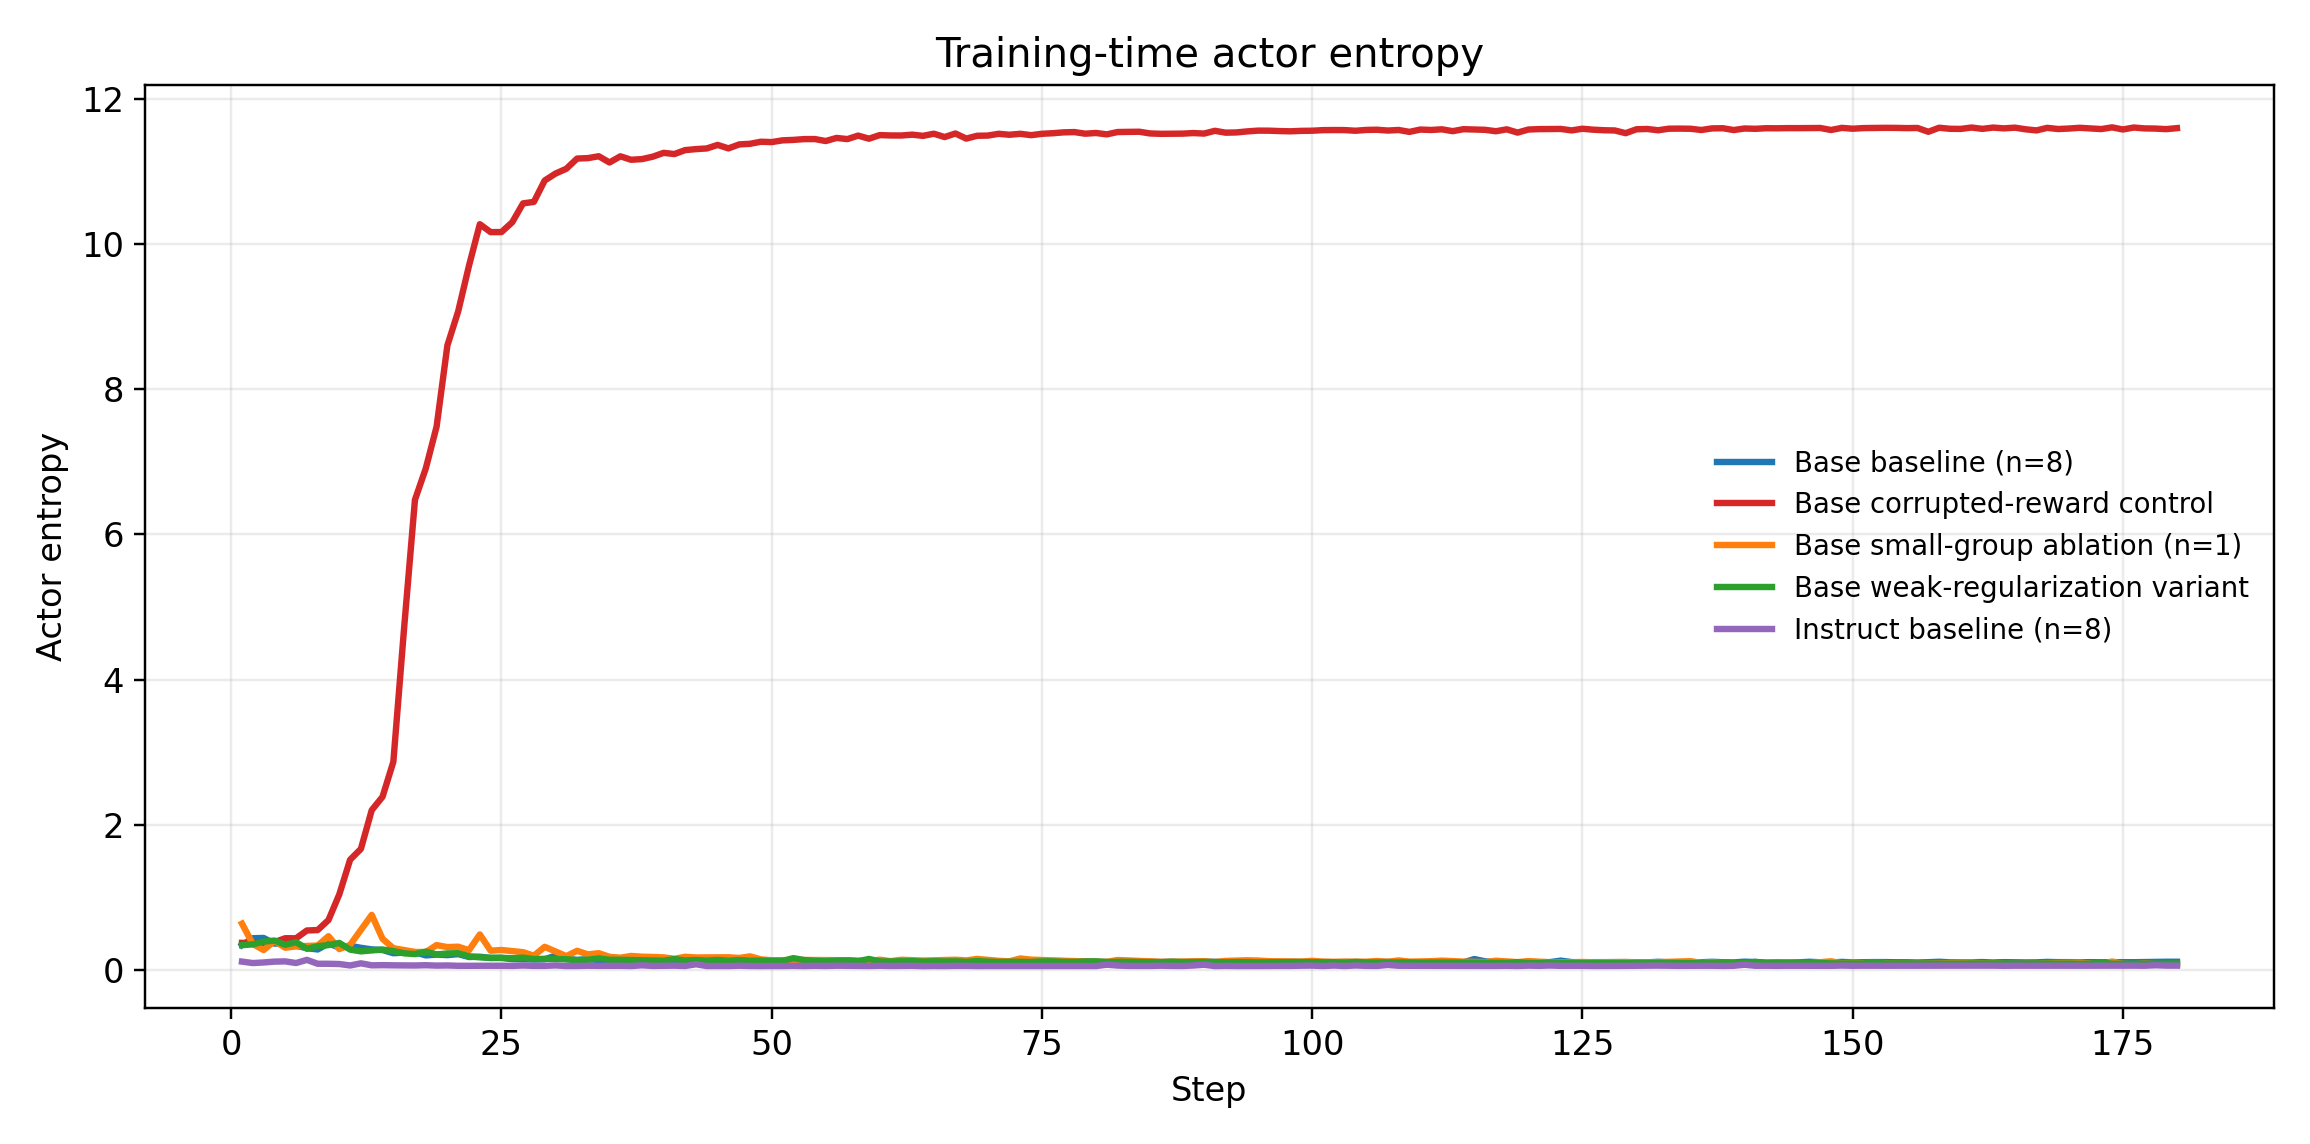
\includegraphics[width=\textwidth]{actor-entropy-static.png}
    \caption{五个正式实验训练期 \texttt{actor/entropy} 变化。Base clean 实验呈现明显分布收缩，而破坏性奖励控制实验则出现快速熵爆炸。}
    \label{fig:actor-entropy-curves}
\end{figure}

\begin{figure}[H]
    \centering
    
\includegraphics[width=\textwidth]{aligned-n1-vs-n8-panel.png}
    \caption{对齐评估口径下，\texttt{Base baseline (n=8)} 与 \texttt{Base small-group ablation (n=1)} 的六项动态对比。可以看到 \texttt{n=1} 仍能提升，但在 score、entropy、top-1 probability 与 stopping behavior 上都落后于 \texttt{n=8}。}
    \label{fig:aligned-n1-vs-n8-panel}
\end{figure}

这张表最清楚地强化了 Base 与 Instruct 的分化。以 \texttt{Base baseline (n=8)} 为例，\texttt{actor/entropy} 从 0.346 降到 0.116，验证 token entropy 从 0.675 降到 0.184，低置信 token 比例从 0.116 降到 0.032，聚合 top-1 概率从 0.851 升到 0.935，验证响应长度则从 812.5 缩短到 603.1。弱约束版本的收缩更激进：对应的最终 \texttt{actor/entropy} 进一步降到 0.091，验证 token entropy 降到 0.156，top-1 概率升到 0.944。与之相对，\texttt{Base corrupted-reward control} 并未出现任何“轻微变差但仍有学习”的形态，而是沿着完全相反的方向发展：\texttt{actor/entropy} 从 0.376 升到 11.594，验证 token entropy 从 0.633 升到 11.547，低置信 token 比例升到 1.000，top-1 概率坍缩到 0.002，验证响应长度则暴涨到 1192.4。也就是说，Base 家族的 clean 收益并不只是最终 reward 提高，而是伴随着训练熵下降、验证熵下降、低置信 token 减少、top-1 概率升高与长度缩短的一整套同步变化；一旦奖励信号被系统性破坏，这整套变化会整体反向。

\texttt{Base small-group ablation (n=1)} 让这个故事更细致了一层。新的对齐版消融在 \texttt{step 0} 为 0.363，最终为 0.547，最佳 step 为 174、best score 为 0.559。也就是说，在与 \texttt{Base baseline (n=8)} 完全一致的验证口径下，把训练 group size 从 8 降到 1 后，模型依然获得了显著收益，但 final score 低了约 0.026，best score 也低了约 0.016。与此同时，它的最终 token entropy 为 0.317，明显高于 \texttt{Base baseline (n=8)} 的 0.202 与 \texttt{Base weak-regularization variant} 的 0.156；低置信 token 比例为 0.051，也高于对应的 0.037 和 0.030；平均 top-1 概率则只有 0.921，低于 \texttt{n=8} 基线的 0.932。图~\ref{fig:aligned-n1-vs-n8-panel} 进一步表明，这种差异不是单个 final checkpoint 的偶然波动，而是贯穿 score、entropy、length 与 top-1 probability 的整体形态差异。更合理的解释是：把 group size 降到 1 不会阻止学习，但会削弱分布收缩与稳定闭合的质量。

Instruct 家族则呈现出另一种模式。\texttt{Instruct baseline (n=8)} 的 \texttt{actor/entropy} 只从 0.118 降到 0.062，验证长度几乎不变，top-1 概率也基本维持在 0.96 附近。这更像局部微调，而不是结构性重整。换句话说，在高先验模型上，当前 one-shot 级别的强化学习更多是在已有稳定分布附近做细节抛光，而不是像 Base 家族那样触发一次明显的分布重排。

\subsection{弱约束版本的启示}

\texttt{Base weak-regularization variant} 的 final score 与标准基线非常接近，但它的最终 entropy 更低、top-1 概率更高、响应也更短。这说明关闭 KL 和 entropy 约束后，模型并没有立刻崩坏，反而朝着更激进的分布收缩方向前进。这里需要谨慎：更激进的收缩既可能意味着“更快收敛到好解法”，也可能意味着“更容易过拟合或更依赖少量样本偏差”。当前报告只能确认它没有显著损伤最终准确率，但不能据此得出“约束项可有可无”的结论。

换句话说，弱约束实验的价值不在于证明约束无用，而在于提醒我们：在极低样本强化学习里，最终分数并不足以代表训练过程的健康程度。若后续要把这组工作写成更完整的论文，最值得补充的是 step-level 波动分析和 representative failure case 分析。

\subsection{Instruct 模型主要是局部微调}

\texttt{Instruct baseline (n=8)} 的最终行为指标呈现出另一种图景。它的 response length 本来就较短，tail confidence 本来就很高，low-confidence token ratio 也处于较低水平。训练后虽然仍然有一定变化，但幅度远小于 Base 模型。例如，它的 entropy 只是在低位小幅波动，EOS probability 始终接近 0.99。这说明 Instruct 模型的主要变化不是从“混乱走向有序”，而是在已有稳定分布上做细节打磨。

这类结果对研究假设非常关键。它说明同样的 1-shot GRPO 并不会以同样方式作用于所有模型。对于先验较弱的 Base 模型，它更多扮演纠偏器；对于先验较强的 Instruct 模型，它更像抛光工具。

\section{Token 级补充证据}

\subsection{补充材料的口径与边界}

除当前正式实验外，仓库中还保留了一份更早的四实验 token 级诊断报告。它并不覆盖全部主实验，而是聚焦于固定题目上的完整轨迹子集。结合当前配置，更准确的理解应当是：每个 step、每个实验最多有 64 个样本参与 token diagnostics 统计，但只有 8 条样本保留完整 token 轨迹，而且每条记录只保留前约 96 个 token。因此，这部分材料更适合作为“机制补充证据”，而不宜被直接外推为“对全部 500 题均成立的统计结论”。

尽管覆盖范围有限，这批 token 轨迹仍然非常有价值。原因在于，它真的保留了 token 位置级的 \texttt{logprob}、\texttt{entropy}、\texttt{top1\_prob} 和 top-k mass 等信息，可以更直接地回答“训练是否在早期 token 组织上做了校正”。需要同时指出的是，本文还额外拥有正式实验共享的聚合 token 摘要曲线，因此 token 证据已经分成两层：一层是正式实验共享的 64-sample 聚合统计，用于支持整体方向；另一层是更早四实验固定题目的完整轨迹，用于展示局部机制。

\subsection{直接观察：Base 变化大，Instruct 变化小}

图~\ref{fig:token-probe-over-steps} 与图~\ref{fig:token-step-metrics} 给出了固定题目上的 token 级可视化结果。可以看到，Instruct 系列在 \texttt{step 0} 就已经具备较高的 token confidence 和较低的 entropy，训练后变化不大；Base 系列则表现出更明显的轨迹收缩和前缀稳定化。尤其在 \texttt{Base-Full} 与 \texttt{Base-OneShot} 的对比中，训练后期的 entropy 降幅和 top-1 概率增幅都清晰可见。

\begin{figure}[H]
    \centering
    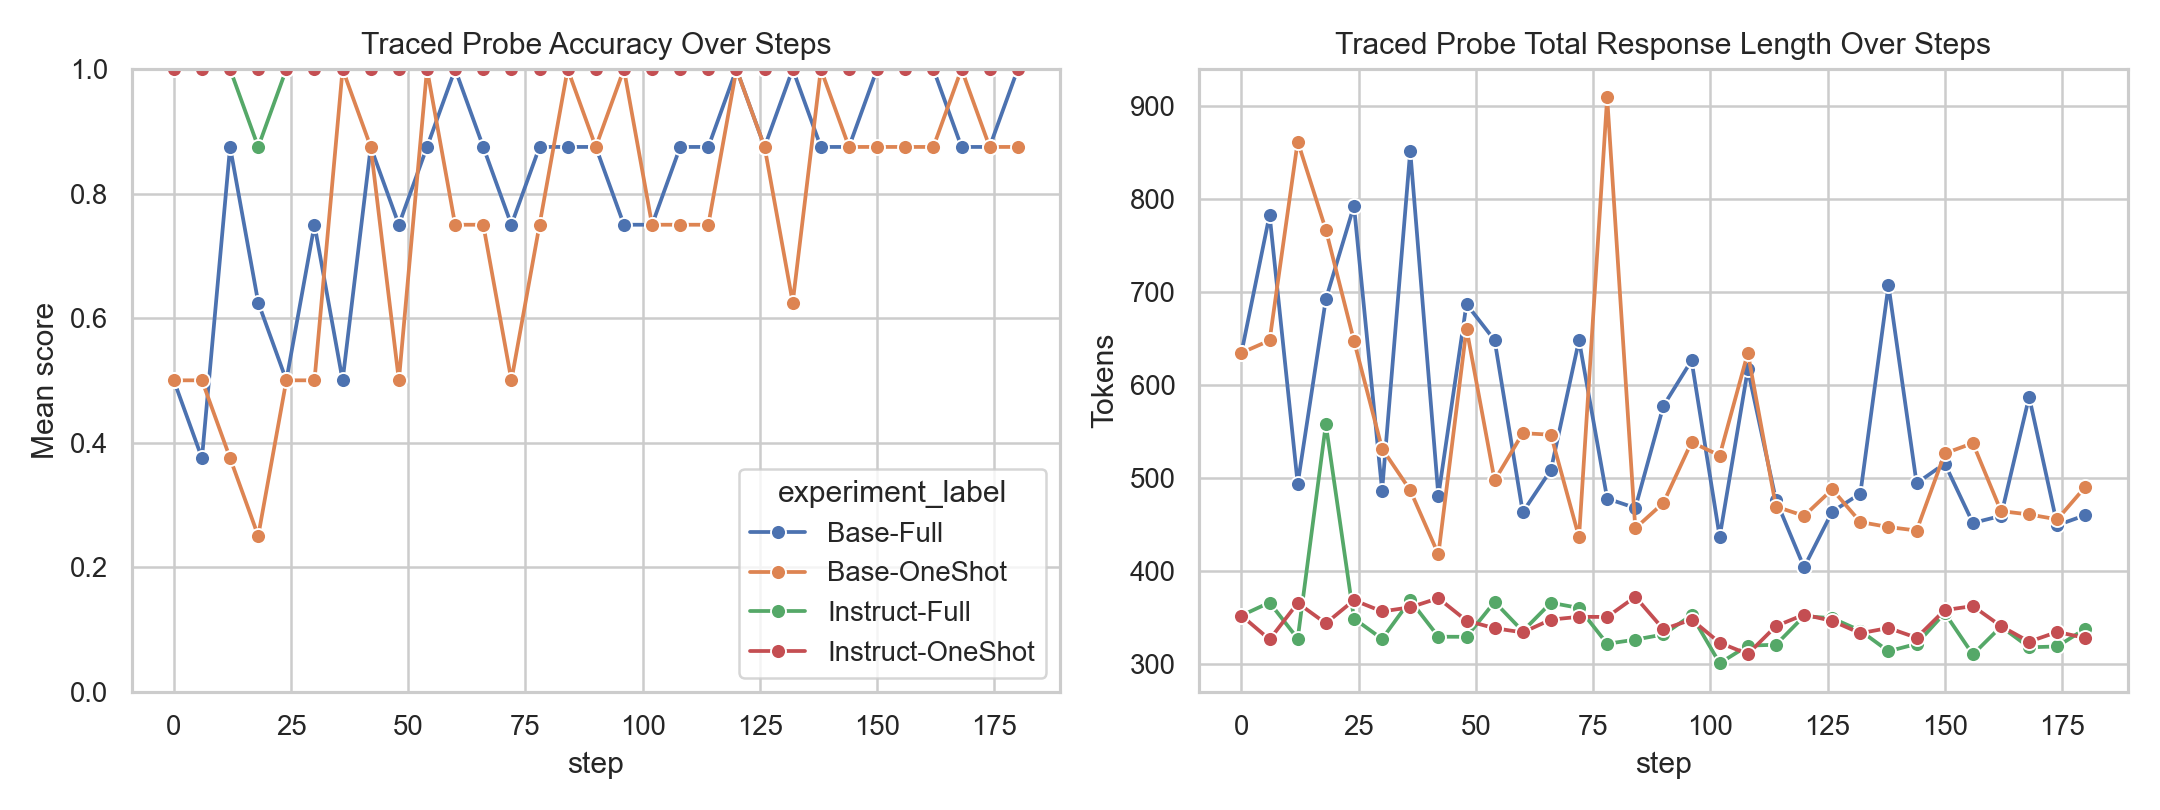
\includegraphics[width=\textwidth]{token-probe-over-steps.png}
    \caption{固定题目在不同 step 上的保留轨迹。该图直观展示了训练后前缀组织与终止行为的变化。}
    \label{fig:token-probe-over-steps}
\end{figure}

\begin{figure}[H]
    \centering
    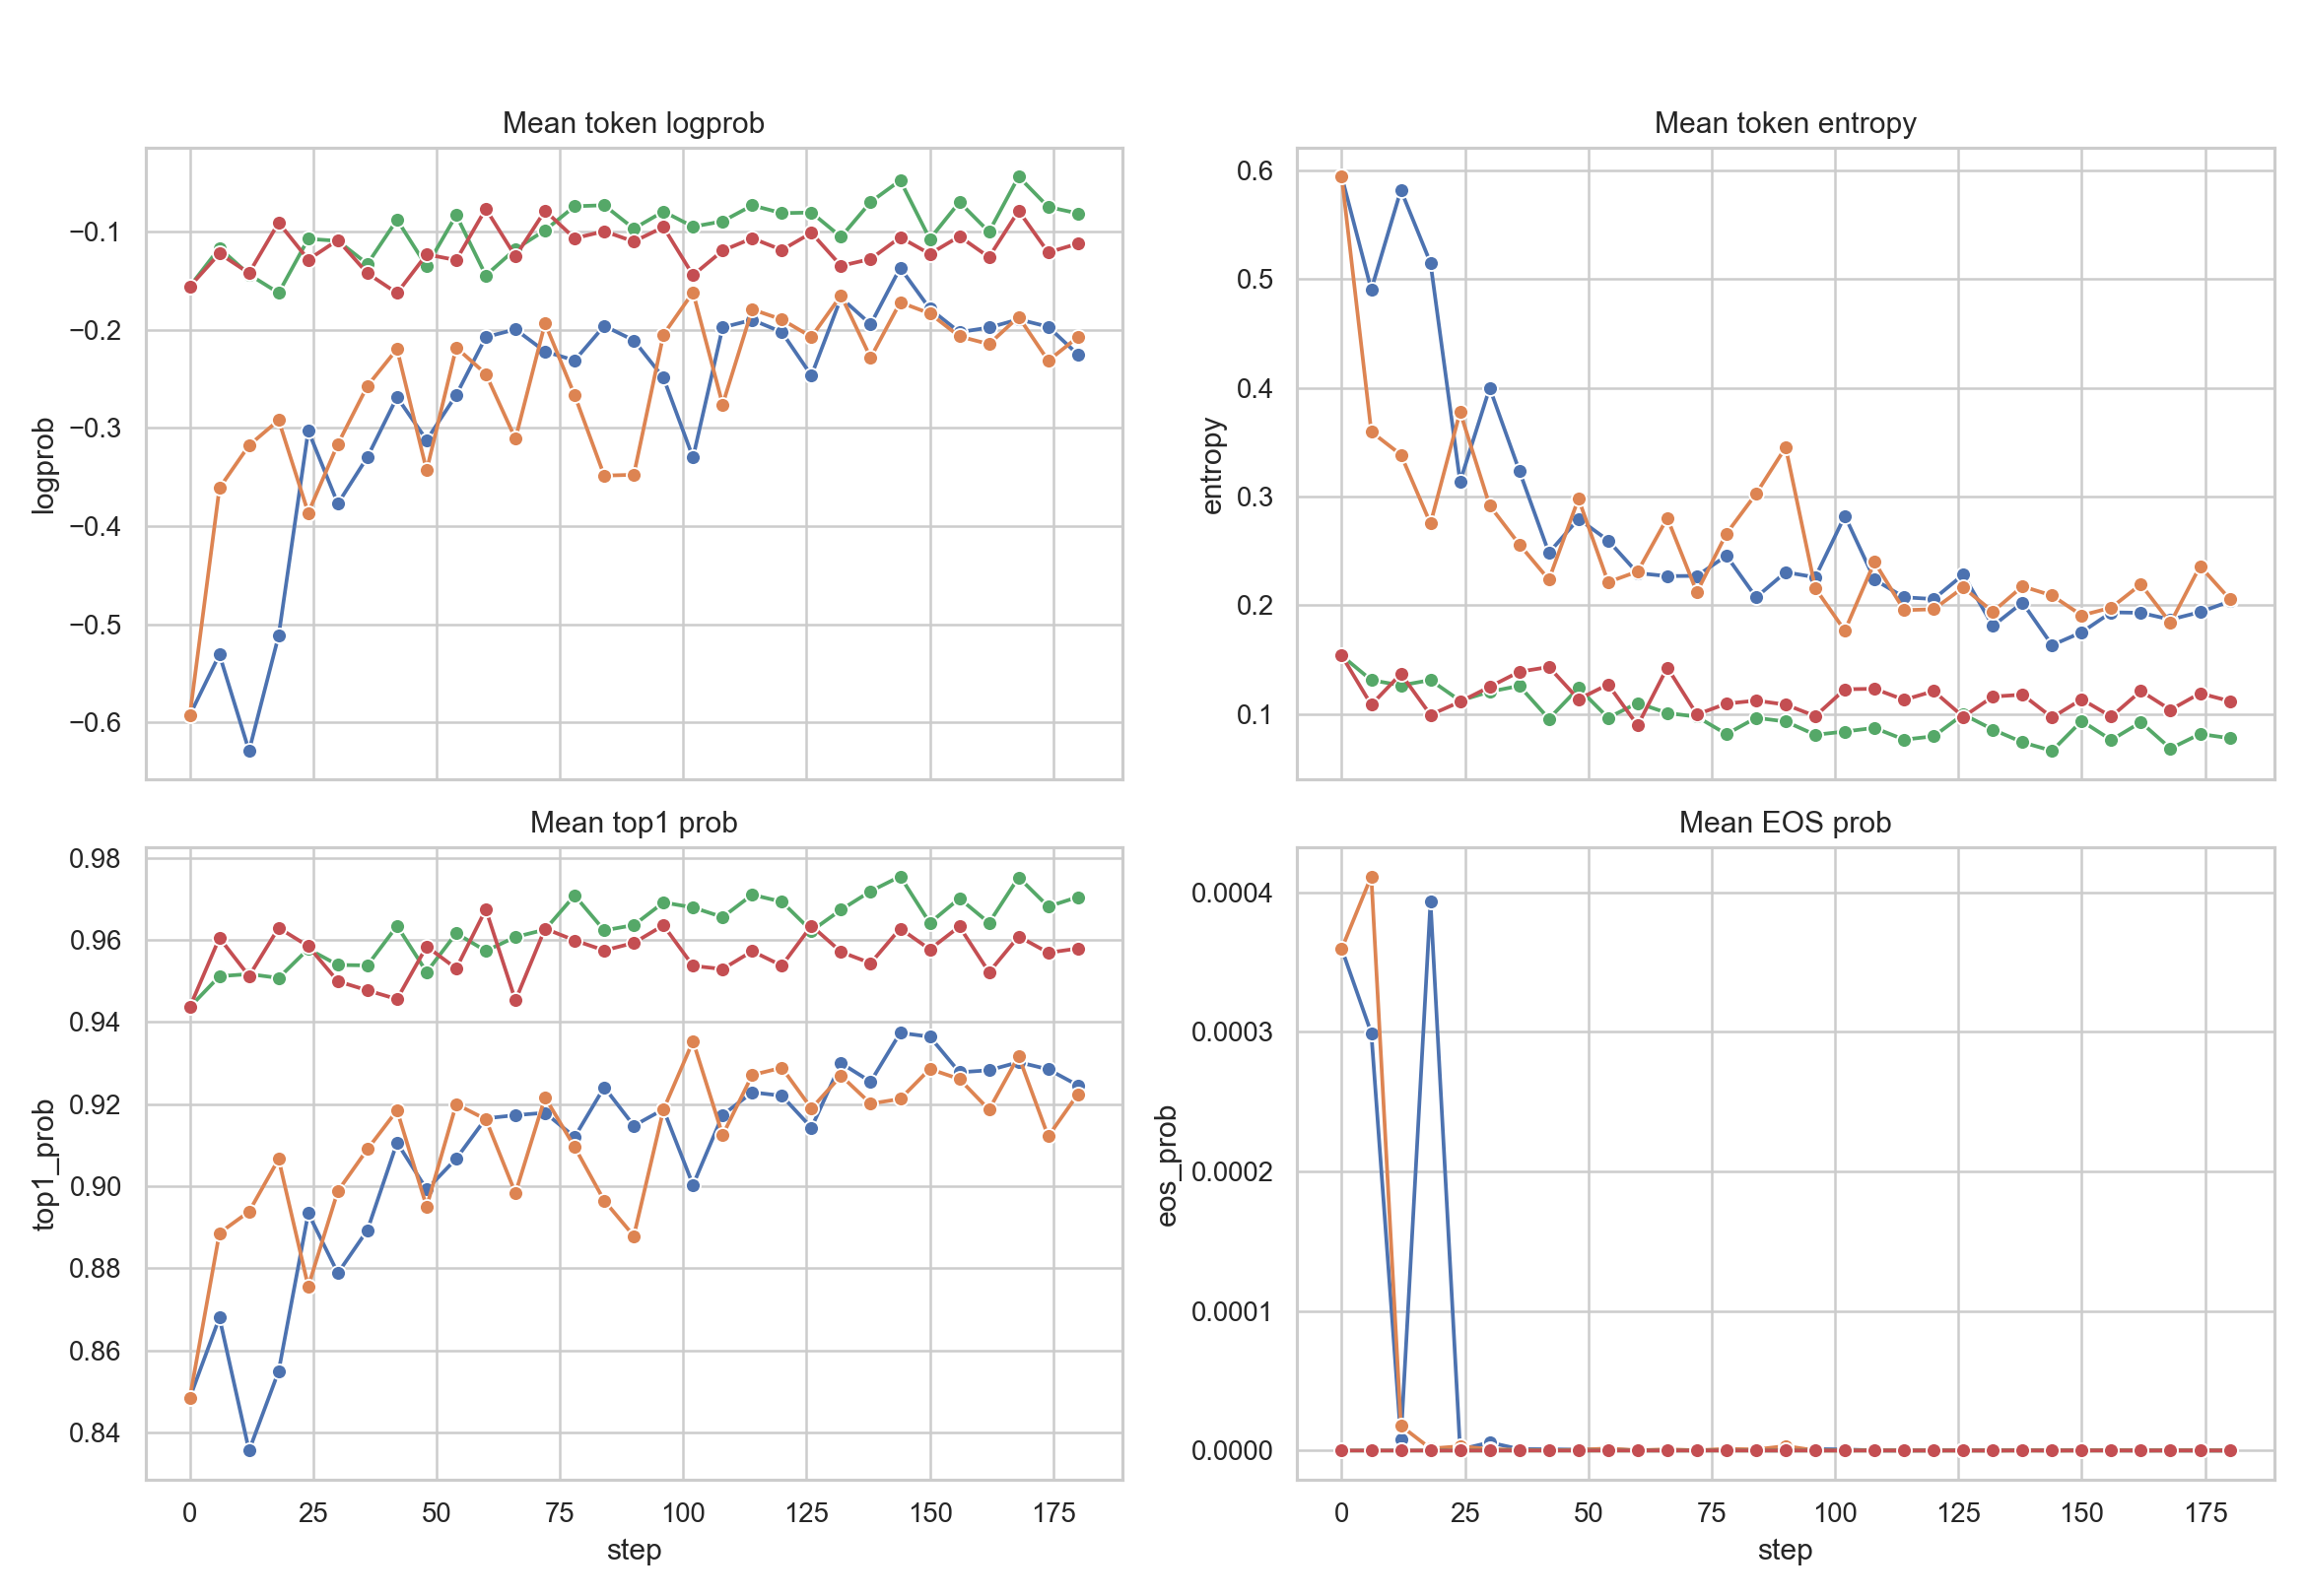
\includegraphics[width=\textwidth]{token-step-metrics.png}
    \caption{固定题目的 token 级熵、概率与长度等指标随 step 的变化。该图更适合支持“训练改变了早期 token 组织方式”的叙事。}
    \label{fig:token-step-metrics}
\end{figure}

表~\ref{tab:token-final} 与表~\ref{tab:token-delta} 进一步给出该固定题目的数字证据。首先，在 final step 上，\texttt{Base-Full} 的平均 entropy 为 0.2036，而 \texttt{Instruct-Full} 仅为 0.0778；对应的 top-1 概率分别为 0.9246 和 0.9705。其次，从 \texttt{step 0} 到 final，\texttt{Base-Full} 与 \texttt{Base-OneShot} 的 logprob 增量和 entropy 下降幅度都远大于 Instruct 系列。这说明 Base 模型的训练变化确实更剧烈，也更像一次明显的行为校准。图~\ref{fig:token-probe-over-steps} 与图~\ref{fig:token-step-metrics} 提供了与这些数值一致的可视化证据。

\begin{table}[H]
    \centering
    \caption{固定题目在 final step 上的 token 级摘要}
    \label{tab:token-final}
    \begin{tabular}{lccccc}
        \toprule
        实验 & correct? & traced tokens & entropy & top1 prob & top5 mass \\
        \midrule
        Base-Full & correct & 768 & 0.2036 & 0.9246 & 0.9970 \\
        Base-OneShot & correct & 672 & 0.2005 & 0.9248 & 0.9970 \\
        Base-OneShot & wrong & 96 & 0.2435 & 0.9056 & 0.9977 \\
        Instruct-Full & correct & 768 & 0.0778 & 0.9705 & 0.9998 \\
        Instruct-OneShot & correct & 768 & 0.1119 & 0.9580 & 0.9996 \\
        \bottomrule
    \end{tabular}
\end{table}

\begin{table}[H]
    \centering
    \caption{固定题目从 \texttt{step 0} 到 final 的 token 级变化量}
    \label{tab:token-delta}
    \begin{tabular}{lccc}
        \toprule
        实验 & $\Delta$ logprob & $\Delta$ entropy & $\Delta$ top1 prob \\
        \midrule
        Base-Full & +0.3673 & -0.3908 & +0.0762 \\
        Base-OneShot & +0.3849 & -0.3885 & +0.0740 \\
        Instruct-Full & +0.0744 & -0.0760 & +0.0268 \\
        Instruct-OneShot & +0.0435 & -0.0419 & +0.0143 \\
        \bottomrule
    \end{tabular}
\end{table}

\subsection{与当前正式实验结论的衔接}

需要强调的是，这些 token 图并不是为了替代正式主结果，而是为了增强主结果的解释力。当前宏观统计已经告诉我们：Base 模型收益大，Instruct 模型收益小；而 token 级补充材料进一步告诉我们：这种差异不是偶然的，而是体现在前缀组织方式、分布收缩和正确结束行为上的。二者放在一起，才能形成一条较完整的证据链。

\subsection{前缀分布如何被重新组织}

如果把 attention 放到最终答案附近，前面的结论已经足够说明“训练后更稳了”；但如果进一步看输出前缀的位置级分布，能够看到更具体的变化方向。图~\ref{fig:prefix-curves-main} 展示了 final step 上不同实验在前缀 token 区域的曲线差异。它的价值在于把“最终答对”拆开为“从一开始是否就沿着更干净的轨道展开”。对于 Base 家族而言，这一点尤其重要，因为它们的改进并不是只发生在最后一两个答案 token 上，而是从更早的前缀阶段就开始体现为更低的熵和更集中的 top-1 概率。

这张图与前面的动态聚合曲线能够相互印证。聚合统计表明，Base 家族在 step-level 上持续收缩；而前缀图进一步说明，这种收缩并不是平均到所有位置后才看得出来，而是在输出早期就已经发生。对于数学推理任务，这意味着模型更快地进入正确的结构化推理轨道，而不是先走一段模糊、犹豫的路径，再在答案末端临时纠正。

\begin{figure}[H]
    \centering
    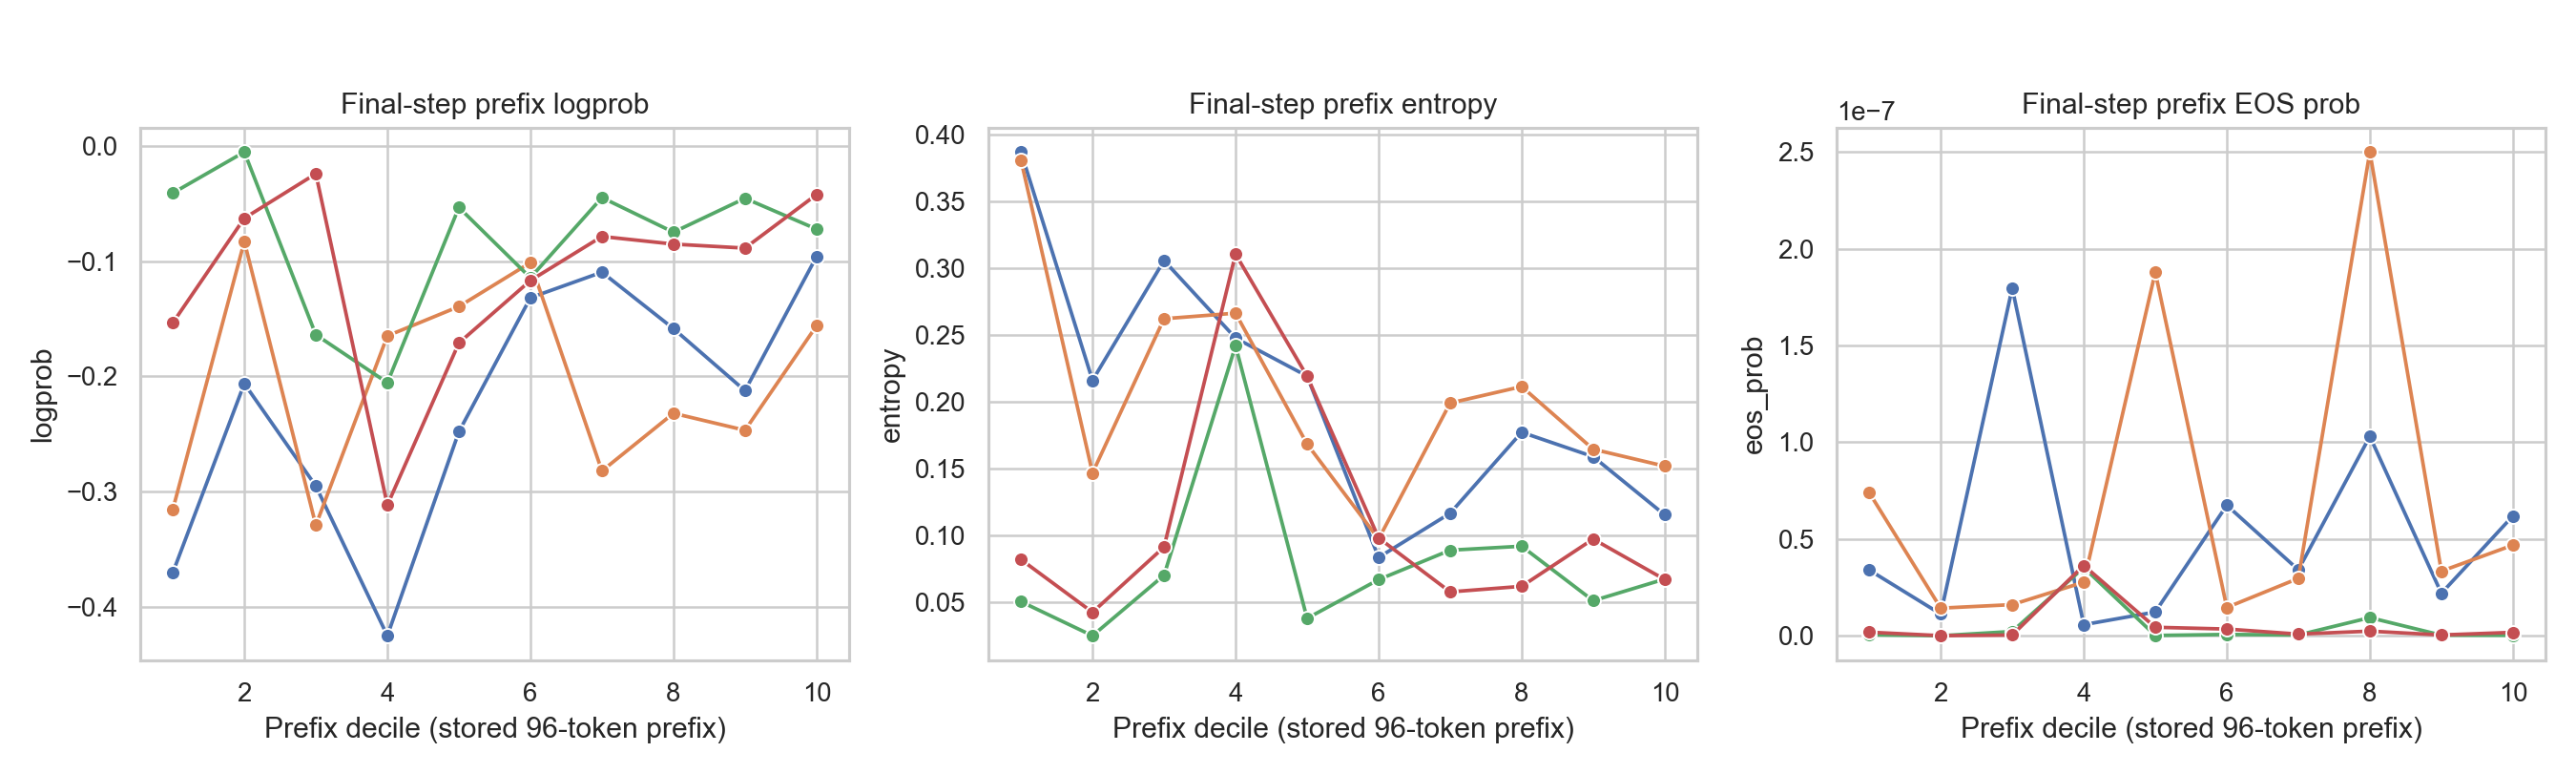
\includegraphics[width=\textwidth]{final-prefix-curves.png}
    \caption{final step 上不同实验在前缀 token 区域的曲线差异。该图用于说明训练后前缀组织本身发生了系统变化，而不仅仅是末尾答案更稳定。}
    \label{fig:prefix-curves-main}
\end{figure}

\subsection{从 \texttt{step 0} 到 final：局部 token 分布到底收缩了多少}

图~\ref{fig:token-delta-main} 把关注点放到训练前后差值本身。相比只看 final step，它更适合回答一个机制问题：模型到底是“整体轻微变好”，还是“某些关键位置发生了明显的分布重排”。从图中可以看到，Base 条件的变化幅度远大于 Instruct 条件，尤其是在早期和中段 token 区域，\texttt{logprob} 上升与 \texttt{entropy} 下降同时出现。这与前文“Base 更像被快速校准，Instruct 更像被局部抛光”的主叙事完全一致。

对对齐版 \texttt{n=1} 消融的理解也可以从这类图里得到补充。虽然当前完整轨迹图本身不是为这条实验单独生成的，但它所呈现的变化模式与正式实验聚合结果相匹配：训练能够让 Base 模型在 token 级分布上变得更稳，而当 group size 缩小后，这种分布清理仍然发生，却不如 \texttt{n=8} 那样充分。也正因为如此，正文里关于 group-relative signal 的判断并不是仅仅依赖一个汇总分数，而是有来自局部 token 变化形态的间接支撑。

\begin{figure}[H]
    \centering
    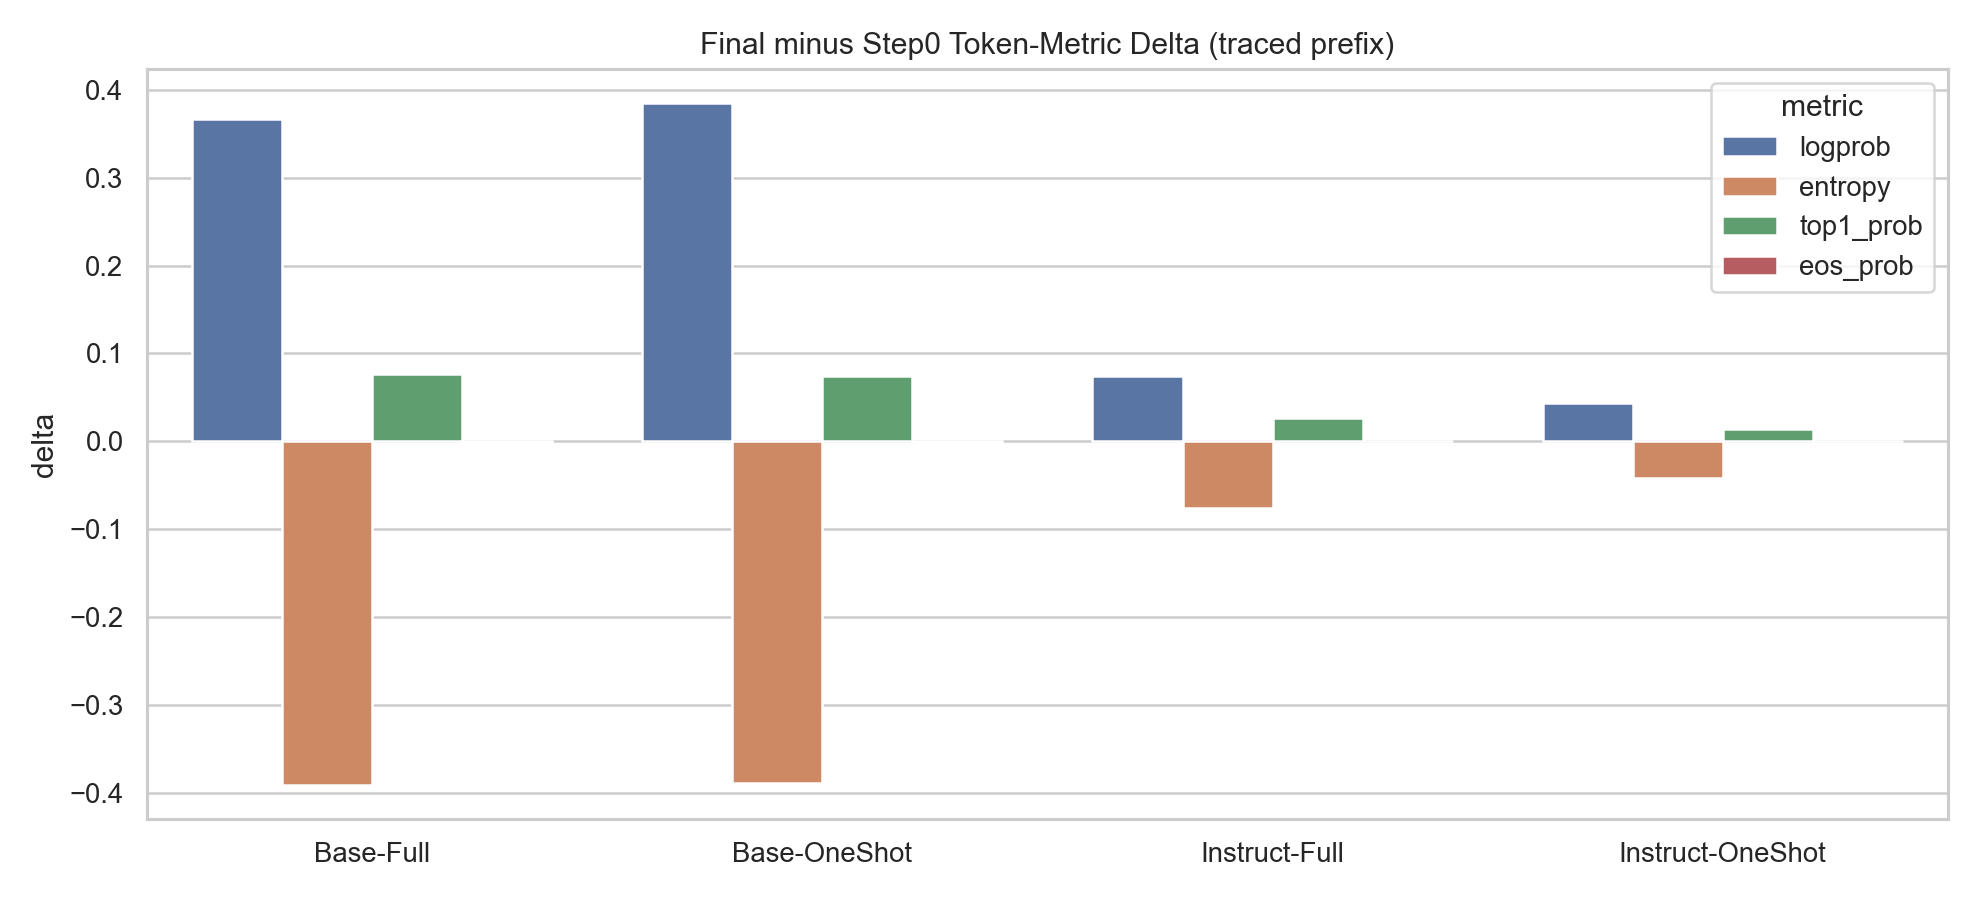
\includegraphics[width=\textwidth]{token-delta-step0-to-final.png}
    \caption{从 \texttt{step 0} 到 final 的 token 级变化。该图强调训练前后局部 token 分布的收缩幅度，尤其适合支撑“快速校准”而非“知识注入”的解释。}
    \label{fig:token-delta-main}
\end{figure}

\subsection{正确与错误响应的分布差异为什么重要}

最后一个经常被忽视的问题是：更低的 token entropy 本身是否真的和更高正确率有关，还是只是一个“看起来更自信”的副产物。图~\ref{fig:correct-wrong-main} 给出了一个直观答案。在固定题目的完整轨迹子集中，正确样本与错误样本在 entropy 上呈现出明显分离，这意味着“分布更稳定”并不是一个与任务无关的美观指标，而是与解题成功概率直接相关的行为特征。

当然，我们仍然不能把这张图写成“全任务层面的严格统计规律”，因为它建立在受限的完整轨迹子集上。但它至少完成了一个关键补充：把正文中已经反复出现的 entropy 收缩，与“为什么这会帮助正确率提升”连接了起来。就论文论证而言，这类桥接图有助于把主分数、行为曲线和机制解释串成一个更闭合的故事。

\begin{figure}[H]
    \centering
    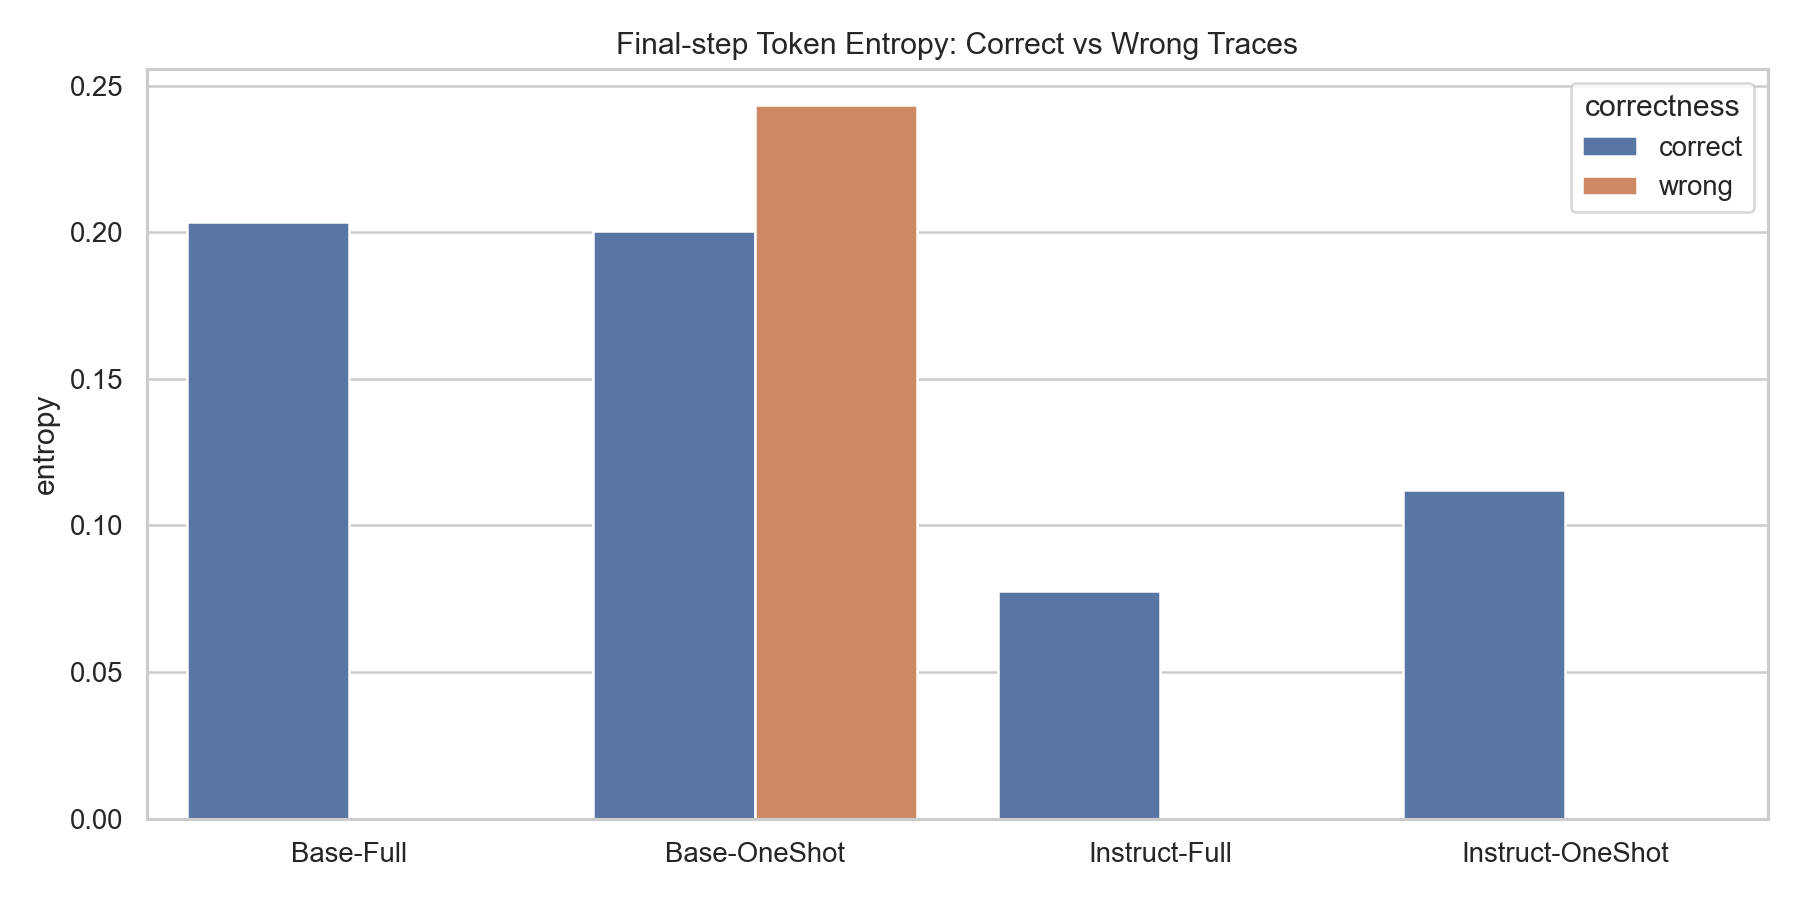
\includegraphics[width=\textwidth]{correct-vs-wrong-entropy.png}
    \caption{正确与错误完整轨迹响应在 token entropy 上的差异。该图用于解释为什么更干净的 token 分布与更高的最终正确率具有一致方向。}
    \label{fig:correct-wrong-main}
\end{figure}

\section{消融与严格控制实验分析}

\subsection{\texttt{n=1} 小组规模消融的解释边界}

\texttt{Base small-group ablation (n=1)} 的新对齐结果给出了比旧版更清晰的答案。它从 0.3630 提升到 0.5470，best score 为 0.5590，说明把 group size 降到 1 仍然可以产生实质收益；但在与 \texttt{Base baseline (n=8)} 完全一致的验证设置下，它稳定落后于 \texttt{n=8} 基线的 0.5733 / 0.5753。这意味着当前证据已经不再支持“group size 可能无关紧要”的说法，而是更支持一个更具体的判断：group-relative signal 不是收益存在与否的必要条件，但它对获得更高、更干净的最终收敛结果是重要的。

当然，这一结论仍应保持正式克制。当前 aligned ablation 仍只有单次正式运行，因此它更适合作为“强支持证据”，而不是“彻底盖棺定论”的多 seed 结论。

\subsection{严格破坏性奖励控制实验的解释意义}

严格控制实验的核心目的，是检验 clean baseline 的收益是否真正依赖于有意义的训练信号。如果把奖励系统性破坏后，模型仍能复现 clean 实验的收益，那么“训练确实利用了有效监督结构”这一解释就会被显著削弱；反之，如果破坏性奖励导致性能和分布同时坍缩，那么 clean baseline 的改善就更可以被解释为对真实训练信号的响应。

\begin{table}[H]
    \centering
    \caption{严格破坏性奖励控制实验的终点行为}
    \label{tab:control-collapse}
    \begin{tabular}{lc}
        \toprule
        指标 & 数值 \\
        \midrule
        final score & 0.00025 \\
        final response length & 1192.4 \\
        final tail confidence & 0.0001 \\
        final low-confidence ratio & 1.0000 \\
        final token entropy & 11.5466 \\
        final EOS probability & 0.0009 \\
        final top-1 probability & 0.0021 \\
        \bottomrule
    \end{tabular}
\end{table}

新的 \texttt{Base corrupted-reward control} 给出了与 clean baseline 完全不同的结果。它从 0.3630 起步，却在训练过程中迅速坍缩到 0.00025；与此同时，响应长度从 762.8 增长到 1192.4，low-confidence token 比例升到 1.000，token entropy 升到 11.5466，EOS 结束概率降到 0.0009，平均 top-1 概率也几乎退化为均匀分布水平。表~\ref{tab:control-collapse} 汇总了这种终点崩解状态。就论文论证而言，这是一条非常关键的证据：当奖励信号被系统性破坏后，模型不仅不会复现 clean baseline 的收益，反而会失去稳定生成能力。由此，正文关于 clean 实验收益来源于真实训练信号的解释获得了显著加强。

\section{训练动态的阶段性分解}

\subsection{收益主要发生在什么阶段}

仅仅知道 final score 很高，还不足以说明训练过程是否健康。更有解释力的问题是：收益到底主要来自前期快速抬升，还是来自后期缓慢累积。图~\ref{fig:phase-gain-breakdown} 把五个正式实验的主分数增量拆成三个阶段：\texttt{0$\rightarrow$36}、\texttt{36$\rightarrow$96} 和 \texttt{96$\rightarrow$180}。这种拆法虽然是经验性的，但足够把“起步纠偏”“中段巩固”和“后期波动”区分开来。

从图中可以看到，Base clean 家族的主要收益集中在前两个阶段，尤其是 \texttt{0$\rightarrow$36} 的快速抬升最为明显。这与本文一直强调的“快速校准”完全一致：模型先被迅速拉出初始的高熵、长拖尾状态，然后在中段继续巩固正确轨道；到了最后阶段，收益变得更有限，甚至主要体现为小范围高位波动。相比之下，Instruct 基线几乎没有可观的阶段性增益，这再次说明其训练并不是一次明显的结构性重排，而更像在高位附近做局部抛光。严格控制实验则沿完全相反方向演化，其坍缩主要发生在训练前中期。

\begin{figure}[H]
    \centering
    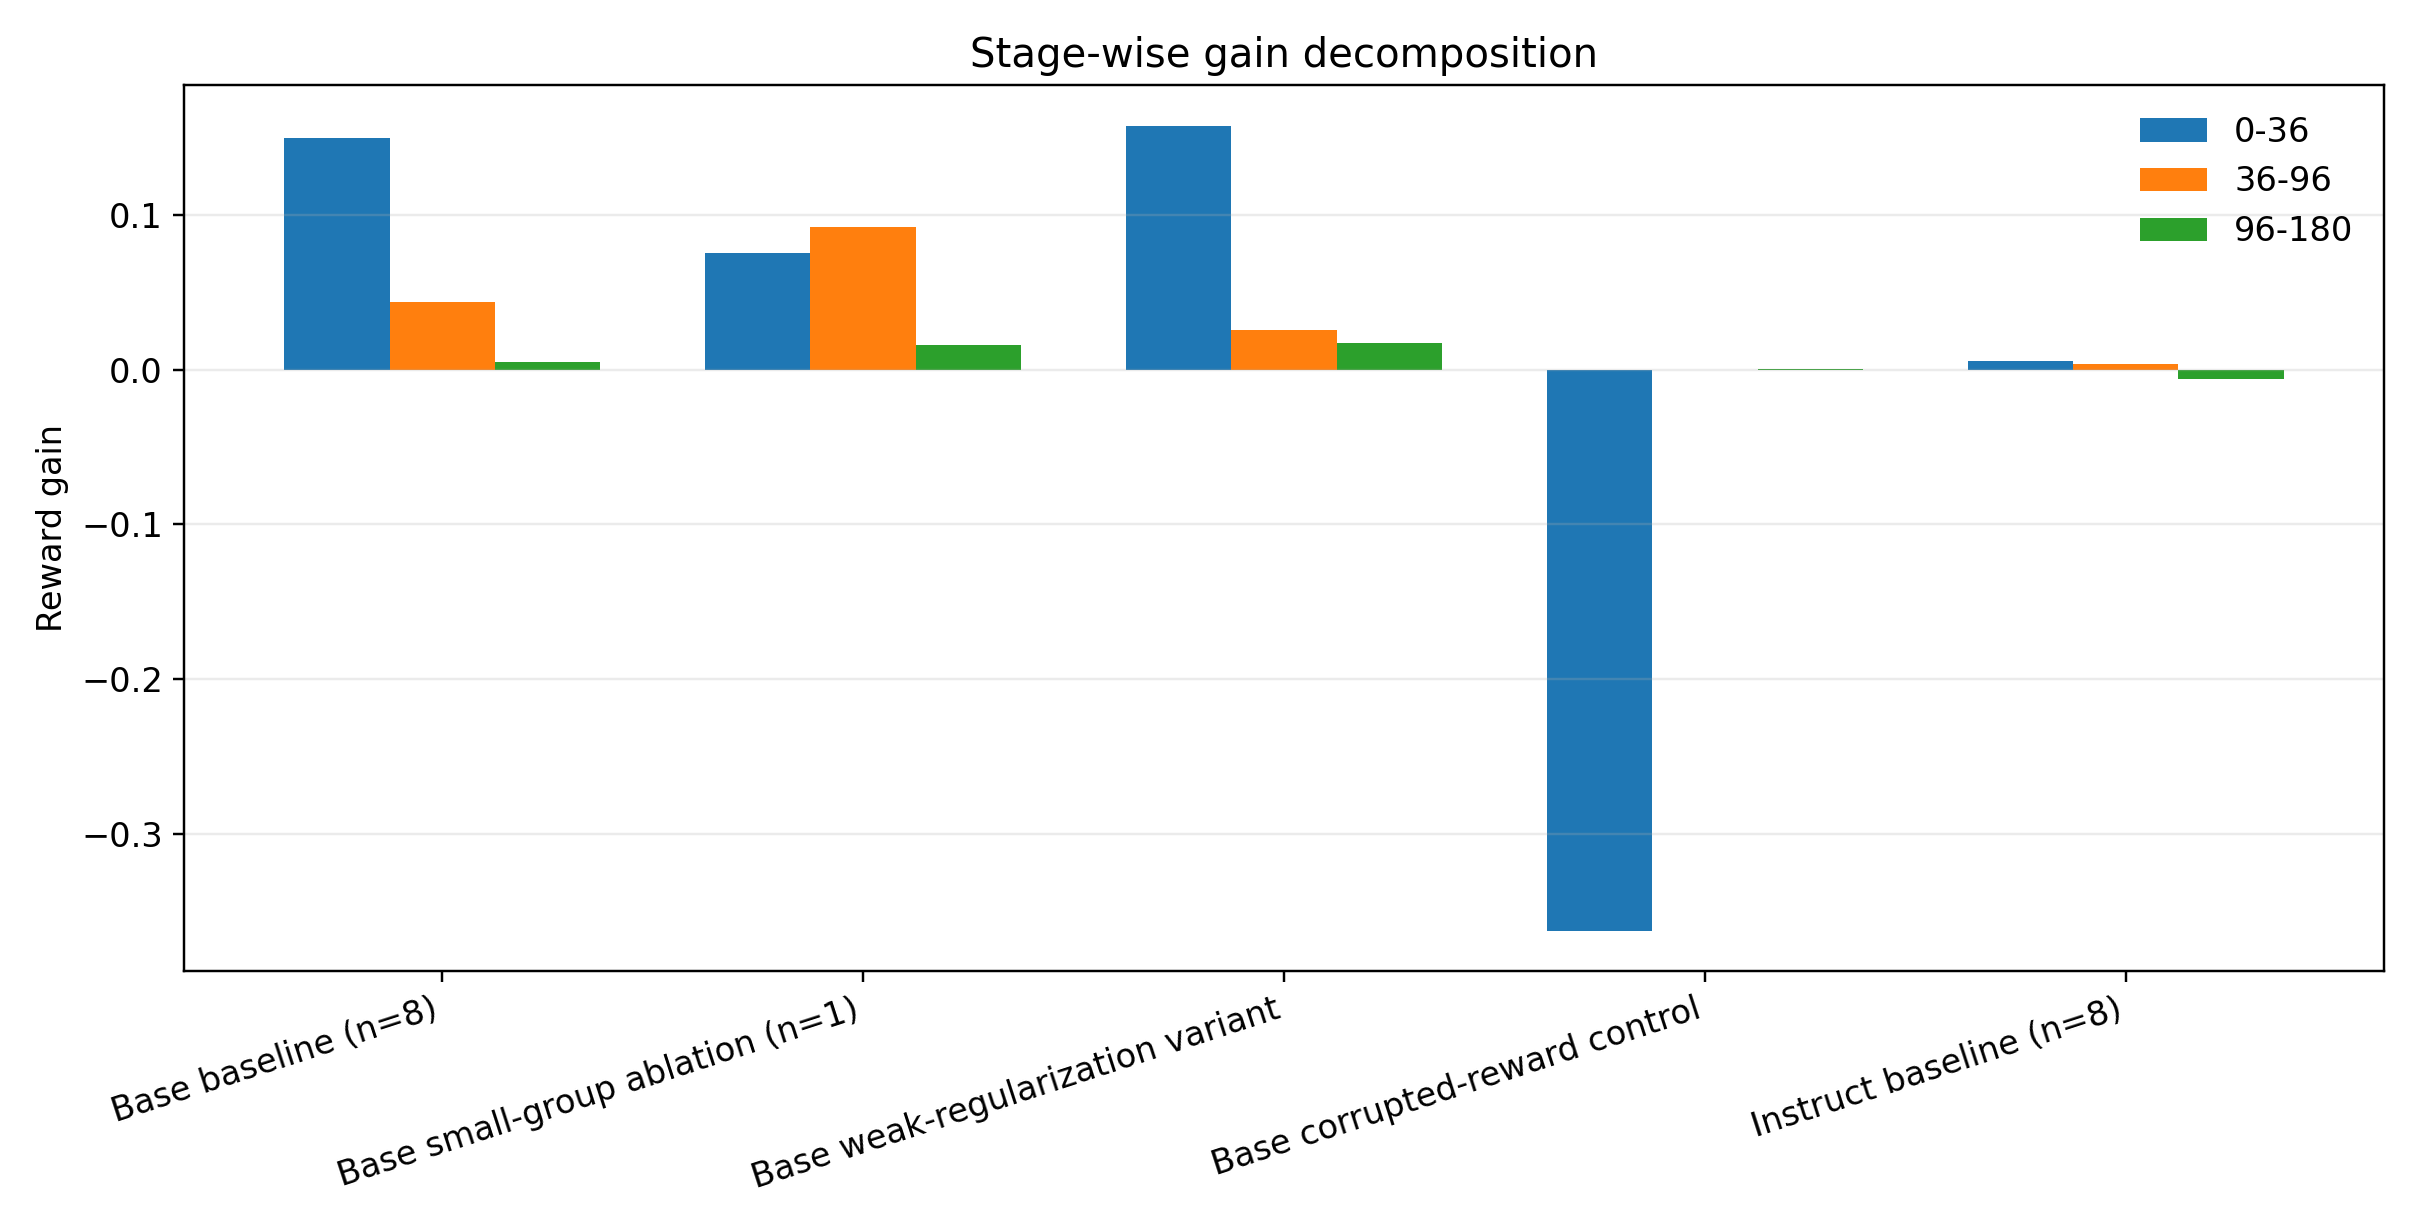
\includegraphics[width=\textwidth]{phase-gain-breakdown.png}
    \caption{五个正式实验主分数增量的阶段性分解。Base clean 实验的收益主要集中在前期纠偏与中段巩固，而严格控制实验呈现持续坍缩。}
    \label{fig:phase-gain-breakdown}
\end{figure}

\subsection{为什么 best checkpoint 和 final checkpoint 不能混为一谈}

在低数据预算强化学习里，最佳点和终点往往并不相同。图~\ref{fig:best-final-gap} 将这个现象拆成两个量同时展示：一是 \texttt{best score - final score} 的差值，二是最佳验证 step 所在的位置。这个图的意义在于，它把前文分散在各处的观察集中起来：虽然多个实验最终都停在 \texttt{step 180}，但真正最优的 checkpoint 常常更早出现。

这个现象对正式报告很关键。它说明当前训练过程更像“快速进入高位区间后在后期轻微振荡”，而不是“越训越好”的单调过程。对 Base 模型而言，这意味着如果任务目标是拿到最佳验证性能，那么早停或 checkpoint selection 都是值得认真讨论的训练策略；对 Instruct 模型而言，则意味着它本来就缺乏大幅收益空间，后期训练更容易表现为噪声而不是确定性的改进。

\begin{figure}[H]
    \centering
    
\includegraphics[width=\textwidth]{best-final-gap.png}
    \caption{五个正式实验的最佳 checkpoint 与最终 checkpoint 对比。左图展示 best-final gap，右图展示最佳验证 step。}
    \label{fig:best-final-gap}
\end{figure}

\subsection{终点行为排序如何补强主叙事}

图~\ref{fig:final-behavior-ranking} 对五个正式实验的若干终点行为指标做了统一排序，包括最终 token entropy、低置信 token 比例、top-1 probability 和响应长度。相比逐个在正文中报数字，这种图更容易看出整体格局。它表明 Base 家族内部虽然都能获得较高收益，但不同实验的“收敛风格”并不完全相同：弱约束版本更激进，标准基线更均衡，对齐后的 \texttt{n=1} 则在最终熵与低置信比例上都落后于 \texttt{n=8}，而严格控制实验则远离所有正常收敛区间。

这个排序图也解释了为什么论文分析不能只看单一 reward。若只看 final score，\texttt{Base weak-regularization variant} 与 \texttt{Base baseline (n=8)} 十分接近；但一旦把终点 token 指标并排观察，就会发现它们在收缩强度、闭合方式和输出长度上其实并不相同。与此同时，\texttt{Base corrupted-reward control} 则把“奖励被破坏后的崩解形态”展示得非常清楚。这个对照说明：当前最有说服力的地方，恰恰在于它把主分数和行为分布放在一起看，而不是停留在单个汇总数字上。

\begin{figure}[H]
    \centering
    
\includegraphics[width=\textwidth]{final-behavior-ranking.png}
    \caption{五个正式实验终点行为指标排序图。该图将 entropy、low-confidence ratio、top-1 probability 和响应长度统一并排展示。}
    \label{fig:final-behavior-ranking}
\end{figure}

\section{多指标之间的耦合关系}

\subsection{收益提升是否真的与校准量同步}

到目前为止，正文已经分别讨论了主分数、行为指标和 token 补充材料，但还有一个更进一步的问题值得直接回答：这些变化之间到底只是“方向上都变好了”，还是在实验级别上也呈现出同步耦合。图~\ref{fig:gain-calibration-coupling} 将五个正式实验的主分数增益，分别与四类动态量的变化幅度并排展示：训练期 \texttt{actor entropy} 的变化量、验证期 token entropy 的变化量、低置信 token 比例的变化量，以及验证响应长度的变化量。

这张图最重要的作用，是把“快速校准”从一种看似合理的叙事，进一步变成一条更闭合的经验事实。Base clean 家族并不只是 reward 提升更大，它们同时也对应更大的 entropy 收缩、更大的低置信 token 减少，以及更明显的长度压缩。Instruct 基线则整体落在另一侧：分数提升小，动态收缩也小。更关键的是，\texttt{Base corrupted-reward control} 落在图中的完全反方向，表现为 reward 下降、熵上升、低置信比例上升以及长度拉长。这种实验级别的同步关系，比单独列出若干最终指标更有说服力，因为它表明“收益”和“分布稳定化”并不是彼此独立的两条观察，而是在同一批 run 上共同出现。

\begin{figure}[H]
    \centering
    
\includegraphics[width=\textwidth]{gain-calibration-coupling.png}
    \caption{五个正式实验的主分数增益与四类关键动态量变化幅度的耦合关系。该图用于说明 clean 收益通常伴随更强的分布收缩与长度压缩，而破坏性奖励控制则沿相反方向移动。}
    \label{fig:gain-calibration-coupling}
\end{figure}

\subsection{终点性能与终点稳定性是否形成共同前沿}

另一个对正式报告很重要的问题是：终点分数更高的实验，是否也总是落在更“稳定”的终点分布上。图~\ref{fig:endpoint-frontier-panel} 将最终验证分数分别与最终 token entropy、最终低置信 token 比例放在同一张图中。虽然只有五个正式实验点，但这种前沿式展示仍然很有价值，因为它把“效果更好”和“分布更稳”压缩到了同一个坐标系里。

可以看到，Base 家族内部基本呈现出清晰趋势：最终分数更高的实验，通常也对应更低的 entropy 与更低的低置信 token 比例。对齐后的 \texttt{Base small-group ablation (n=1)} 在这两个坐标上都明显落后于 \texttt{Base baseline (n=8)}，因此它的劣势不是只体现在某一条 reward 曲线上，而是体现在终点分布质量本身。Instruct 家族则落在另一块区域：它们整体分数更高，但内部变化幅度有限，说明其收益空间本来就不大。这种“不同家族占据不同区域、同一家族内部再沿稳定化方向细分”的形态，让全文的主叙事更加完整。

\begin{figure}[H]
    \centering
    
\includegraphics[width=\textwidth]{endpoint-frontier-panel.png}
    \caption{最终验证分数与最终稳定性指标的联合前沿图。左图为 final score 与 final token entropy，右图为 final score 与 final low-confidence ratio。}
    \label{fig:endpoint-frontier-panel}
\end{figure}

\subsection{为什么这组图对正文是必要的}

如果把这些新图与前文合在一起看，全文的证据组织就不再只是“先给一张 reward 曲线，再补几张行为图”，而是形成了更严密的三层结构。第一层是主分数与 best checkpoint，说明训练确实带来了可观收益；第二层是长度、entropy、top-1 probability、EOS 和 low-confidence ratio 的动态变化，说明收益伴随可解释的行为重排；第三层就是本节的耦合图和前沿图，它们把不同指标重新放回实验层面上联合观察，从而证明这些现象在实验层面也是同步的。对正式论文写作而言，这样的结构不仅更充实，也更接近完整论证的写法。

\section{讨论与局限性}

\subsection{当前最强的证据是什么}

本报告最强的证据并不是单个分数，而是一组相互支撑的现象：Base 模型的正确率显著提升，响应长度缩短，尾部置信度提升，低置信 token 比例下降，token entropy 下降，EOS 概率上升，token 级补充材料中也能看到前缀组织和分布收缩的明显改善。这些现象并不随机，而是共同指向同一个解释：1-shot GRPO 对 Base 数学推理模型的主要作用，是把已有能力更快地校准到更稳定的输出轨道上。

\subsection{当前最弱的地方是什么}

相对而言，当前最弱的部分也很明确。第一，虽然 aligned \texttt{n=1} 消融已经显著提升了 group size 结论的可信度，但它仍是单次正式运行，尚未形成多 seed 稳健性证据。第二，严格的破坏性奖励控制目前只覆盖 Base 家族，尚缺与之匹配的 Instruct 控制版本。第三，token diagnostics 在当前正式实验中虽然覆盖到每个 step 的 64 个诊断样本，但完整 token 轨迹只对其中 8 条样本落盘，因此宏观结论仍应主要建立在逐样本验证均值上，而不是依赖少量固定题目的 token 轨迹。

\subsection{对后续工作的直接建议}

如果要把这份报告继续推进为更强的研究稿件，最值得补的工作有三项。其一，对 aligned \texttt{n=1} 与 \texttt{n=8} 对比补做多 seed 重复，以确认当前 group size 差异不是单次运行噪声。其二，为 Instruct 家族补做与 Base 严格对应的破坏性奖励控制。其三，扩大 token diagnostics 的覆盖范围，从“单一固定题目追踪”扩展到多题目、多 step 的更稳定统计。只要这三项补齐，当前报告中的很多谨慎表述都可以进一步收束成更强结论。

\subsection{当前证据链的正式汇总}

为了避免正文在最后阶段重新退化成孤立的汇总数字，表~\ref{tab:evidence-status} 对当前最重要的四条判断做了一次正式收束。它的作用不是重复前文，而是明确哪些结论已经足够稳，可以写进摘要和结论；哪些结论虽然方向明确，但仍需带着 caveat 表达。这类总结表格的价值在于，它把“结果”“机制”“边界”和“后续工作”放在了同一张图景里。

\begin{table}[H]
    \centering
    \caption{当前关键结论的证据状态汇总}
    \label{tab:evidence-status}
    \small
    \begin{tabularx}{\textwidth}{>{\raggedright\arraybackslash}p{0.25\textwidth}>{\raggedright\arraybackslash}p{0.31\textwidth}>{\raggedright\arraybackslash}p{0.15\textwidth}>{\raggedright\arraybackslash}X}
        \toprule
        结论判断 & 主要证据 & 当前强度 & 仍需保留的边界 \\
        \midrule
        1-shot GRPO 对 Base 数学推理模型有效 & 正式实验主分数曲线、Base clean 家族约 0.20 的绝对提升、行为指标同步改善 & 强支持 & 仍需更多 seed 检验其跨随机初始化的稳定性 \\
        收益更像快速校准而非知识注入 & response length 缩短、entropy 下降、low-conf 降低、top-1 与 EOS 上升、固定题目轨迹证据支持 & 强支持 & token 完整轨迹仍是小规模完整轨迹子集，机制证据主要是“强一致”而非“全覆盖” \\
        group-relative signal 对最佳结果有帮助 & 对齐版 \texttt{n=1} 消融在 matched validation protocol 下稳定落后于 \texttt{n=8} 基线 & 中强支持 & 目前仍是单次 aligned run，尚缺多 seed 复验 \\
        破坏性奖励会破坏训练收益与分布稳定化 & Base 严格控制实验中 score 坍缩、entropy 爆炸、low-conf 饱和、EOS 与 top-1 置信度崩解 & 强支持 & 当前该结论仅在 Base 家族上完成验证 \\
        \bottomrule
    \end{tabularx}
\end{table}

\section{结论}

本文基于当前可核验的五个正式实验产物，对 1-shot GRPO 在数学推理模型上的作用进行了系统整理。结果表明，在 \ModelBase{} 上，1-shot GRPO 可以带来接近 0.20 的显著分数提升，并伴随明显的行为稳定化：更短的响应、更高的尾部置信度、更低的 token entropy、更少的低置信 token 以及更果断的结束行为。与之相对，\ModelInstruct{} 由于起点更高，收益空间明显更小，训练效果更接近高位微调。

因此，当前最值得保留的结论是：1-shot GRPO 在 Base 数学推理模型上是有效的，而它的主要收益更像快速校准而非知识注入。与此同时，新的 aligned \texttt{n=1} 小组规模消融已经提供了更强的机制证据：把训练 group size 从 8 降到 1 会削弱但不会消除收益，这说明 group-relative signal 对最佳效果具有重要贡献。更关键的是，新的严格破坏性奖励控制实验表明，一旦奖励信号被系统性破坏，模型不仅不会复现 clean baseline 的收益，反而会在分数与行为分布上同步崩解。基于此，正文关于 clean 实验收益依赖于真实训练信号的解释已经具备较强说服力。这种结论虽然克制，却也更可靠，更适合当前这组实验所能支撑的证据强度。

\clearpage
\appendix

\section{附录：补充讨论}

\tightparagraph{关于 Base 模型收益的补充说明}
在当前设置下，1-shot GRPO 对 Base 数学推理模型的作用主要体现为行为分布的稳定化，而非简单拉长推理链。模型在训练后显著缩短输出长度、降低 token entropy、减少低置信 token，并更果断地结束答案，这些现象共同支持“快速校准”解释。

\tightparagraph{关于 Instruct 模型收益较小的补充说明}
Instruct 模型在 \texttt{step 0} 已经具备较高的数学推理先验，因此 1-shot GRPO 的作用更接近局部微调与分布抛光，而不是大幅纠偏。这也是其收益量级明显小于 Base 模型的主要原因。

\tightparagraph{关于 \texttt{n=1} 结果的补充说明}
\texttt{n=1} 小组规模消融结果说明，将 group size 降到 1 并不会阻止模型获得显著收益；但在与 \texttt{n=8} 基线对齐的评估口径下，它仍然系统性落后于 \texttt{n=8}，因此当前证据更支持“group-relative signal 对最佳效果有帮助”这一判断。

\tightparagraph{关于严格控制实验的补充说明}
新的 Base 严格控制实验直接采用随机错误奖励构造破坏性监督。结果显示，模型在该设置下不仅无法复现 clean baseline 的收益，反而出现分数坍缩、熵爆炸、长度异常增长与停止行为失稳。这说明正文中的 clean 收益确实依赖于有意义的训练信号，而不是训练流程本身的偶然产物。

\tightparagraph{关于更早阶段历史参考实验的补充说明}
除正文正式实验外，更早阶段的归档实验也提供了一组有价值的补充参照。它们虽然不宜并入主结果表，但能够增强论文对“训练模式差异”和“奖励结构差异”的讨论。表~\ref{tab:legacy-reference-runs-cn} 汇总了其中最具代表性的几条参考结果。整体上看，早期 Base 家族中 \texttt{full} 训练明显强于 \texttt{1-shot}；Instruct 家族中也存在同方向差异，但绝对幅度更小。与此同时，一个格式约束主导的早期参考实验仅从 0.3630 提升到 0.4490，明显弱于常规奖励路径，这使其适合作为正文外的辅助参照。

\begin{table}[H]
    \centering
    \caption{更早阶段历史参考实验汇总}
    \label{tab:legacy-reference-runs-cn}
    \small
    \begin{tabular}{lcccc}
        \toprule
        模型家族 & 设置 & step0 & final & best \\
        \midrule
        Base & 1-shot & 0.3630 & 0.5753 & 0.5803 \\
        Base & full & 0.3630 & 0.6053 & 0.6135 \\
        Base & 格式约束主导参考 & 0.3630 & 0.4490 & 0.4785 \\
        Base & 1-shot entropy 参考 & 0.3630 & 0.5698 & 0.5835 \\
        Instruct & 1-shot & 0.6860 & 0.6928 & 0.6985 \\
        Instruct & full & 0.6860 & 0.7070 & 0.7070 \\
        Instruct & 1-shot 早期参考 & 0.6860 & 0.6893 & 0.7005 \\
        Instruct & full 早期参考 & 0.6795 & 0.7118 & 0.7118 \\
        \bottomrule
    \end{tabular}
\end{table}

\begin{figure}[H]
    \centering
    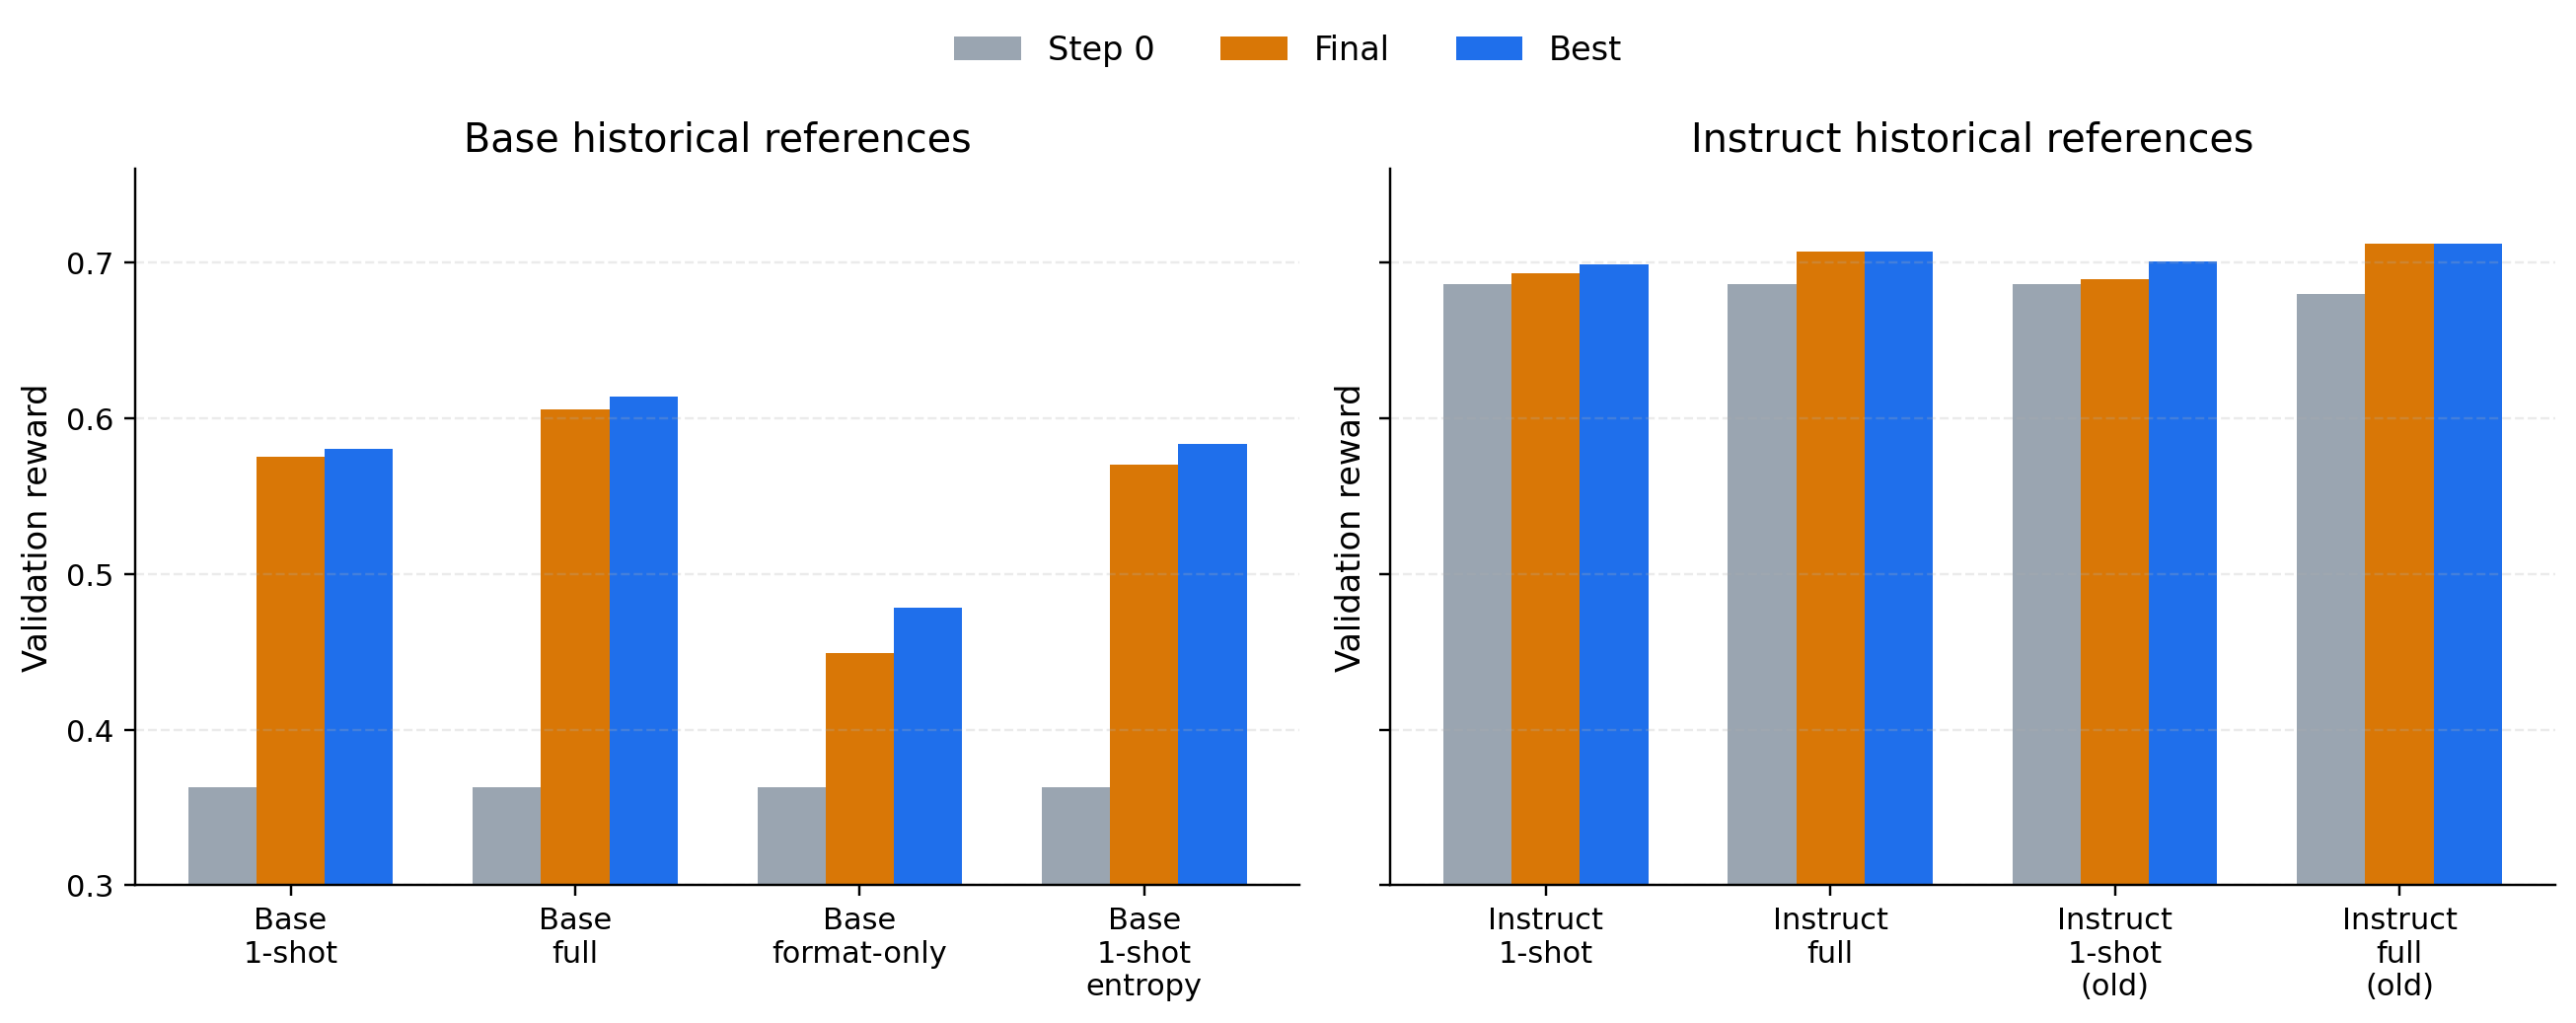
\includegraphics[width=\textwidth]{legacy-reference-panel.png}
    \caption{更早阶段历史参考实验的 step0、final 与 best 对比。该图表明，无论在 Base 还是 Instruct 家族中，\texttt{full} 训练通常都优于 \texttt{1-shot}；同时，Base 家族中的格式约束主导参考明显弱于常规奖励路径。}
\end{figure}

这些实验更适合作为附录层面的历史参考，而不应与正文主矩阵直接合并，原因在于它们所处的实验阶段更早，训练文件范围与记录覆盖也不完全一致。更稳妥的写法是把它们作为“与主结论同向的补充证据”：一方面，\texttt{full} 普遍优于 \texttt{1-shot}；另一方面，格式约束较强的参考设置只能带来有限改善，这与正文中“奖励结构和组内比较信号都会影响最终上限”的主线是一致的。配合上述图表可以更直观地看到，Base 家族对训练范式和奖励结构更敏感，而 Instruct 家族的收益整体更温和。

\section{附录：补充图}

\begin{figure}[H]
    \centering
    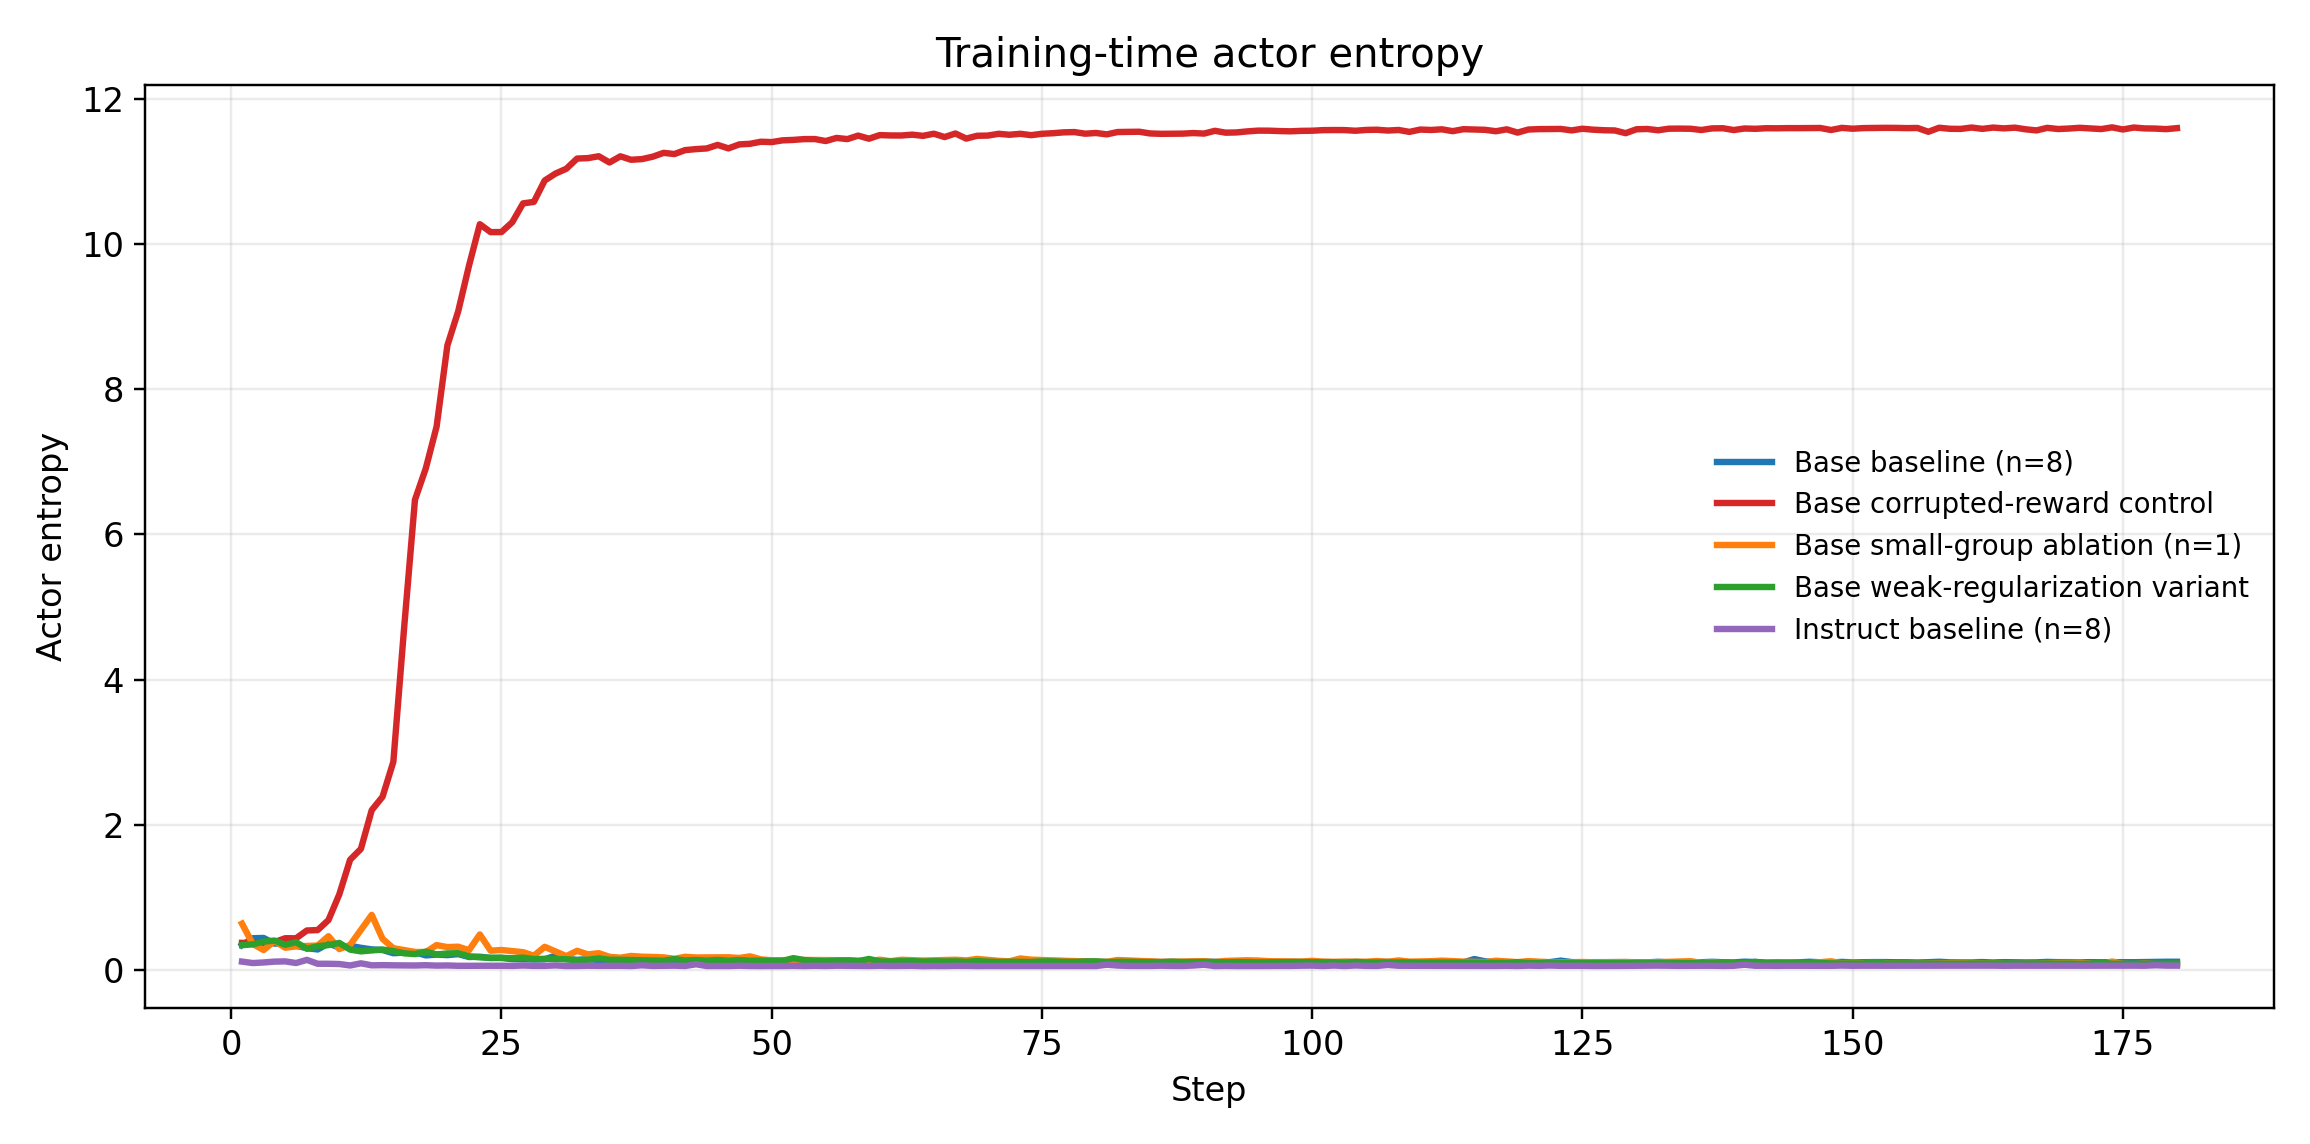
\includegraphics[width=\textwidth]{actor-entropy-static.png}
    \caption{五个正式实验训练期 \texttt{actor/entropy} 的完整补充图。该图可直接作为“训练分布收缩速度与失稳方向”证据使用。}
\end{figure}

\begin{figure}[H]
    \centering
    
\includegraphics[width=\textwidth]{aligned-n1-vs-n8-panel.png}
    \caption{对齐版 \texttt{n=1} 消融与 \texttt{n=8} 基线的多指标对比图。该图可直接用于说明 group size 下降后收益虽保留但分布收缩质量下降。}
\end{figure}

\begin{figure}[H]
    \centering
    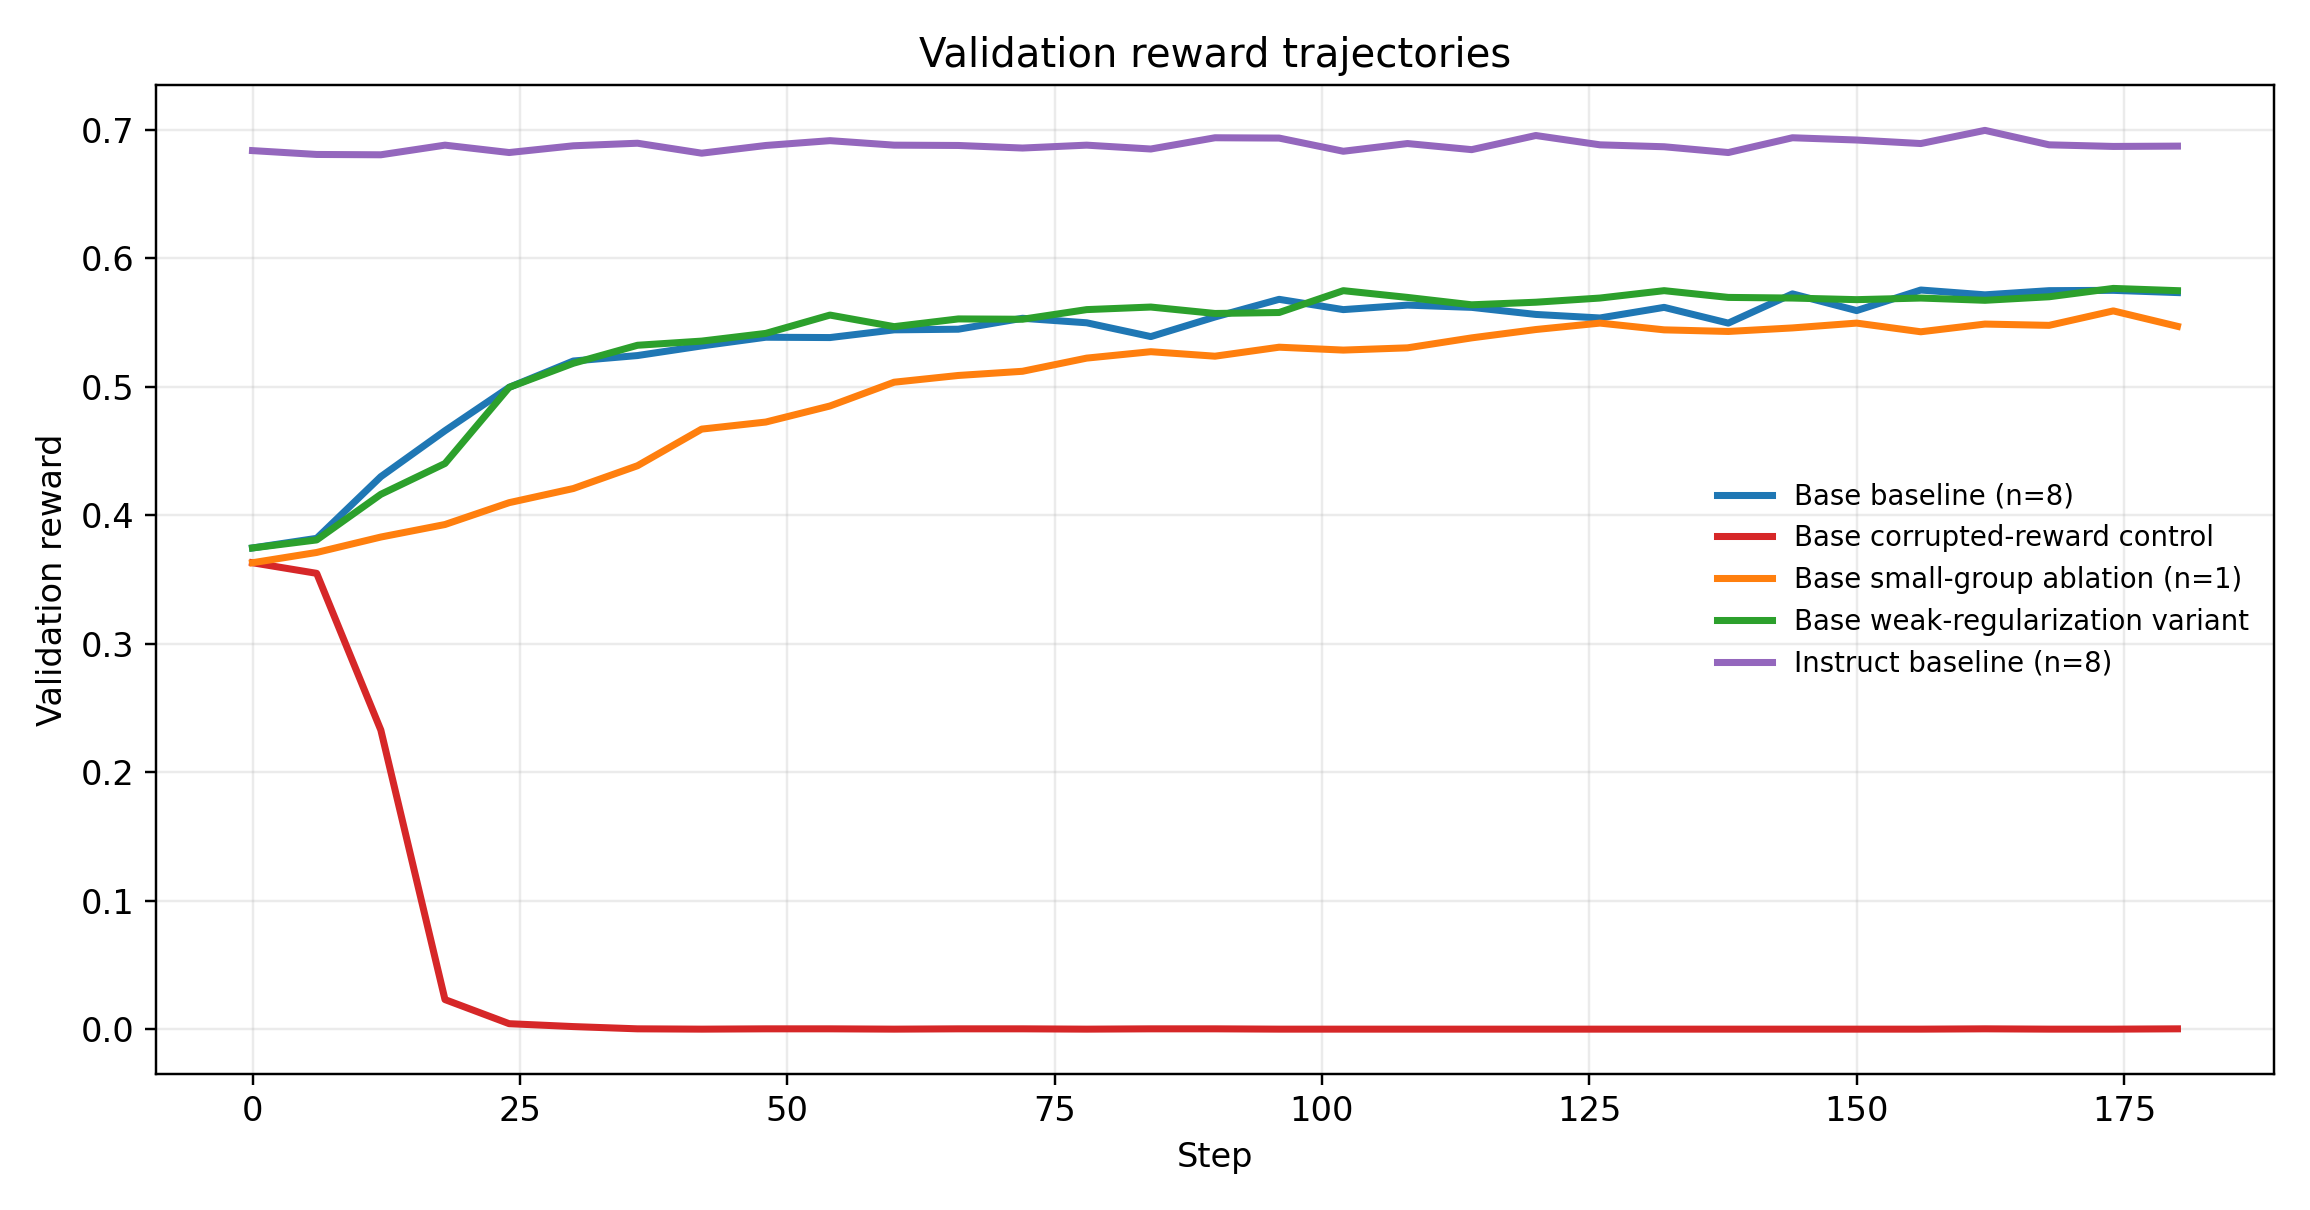
\includegraphics[width=\textwidth]{score-all-static.png}
    \caption{五个正式实验主分数曲线总览补图。该图适合在答辩或补充材料中单独展示总体收益格局。}
\end{figure}

\begin{thebibliography}{99}
\bibitem{ppo}
Schulman, J., Wolski, F., Dhariwal, P., Radford, A., \& Klimov, O. Proximal Policy Optimization Algorithms. arXiv preprint arXiv:1707.06347, 2017.

\bibitem{deepseekmath}
Shao, Z. et al. DeepSeekMath: Pushing the Limits of Mathematical Reasoning in Open Language Models. arXiv preprint arXiv:2402.03300, 2024.

\bibitem{math}
Hendrycks, D. et al. Measuring Mathematical Problem Solving With the MATH Dataset. NeurIPS, 2021.

\bibitem{qwen}
Qwen Team. Qwen2.5 Technical Report. 2024.
\end{thebibliography}

\end{document}
